\documentclass{ufsc-thesis}
\usepackage[utf8]{inputenc}

\title{Estudo de caso de um programa baseado no modelo de atores para teste e diagnóstico de circuitos eletrônicos}
\author{Antonio Carlos Luppi Junior}
\date{Dezembro 2016}
\local{Florianópolis}
\orientador{Fernando Rangel de Sousa}
%\coorientador{Equipe \abnTeX}
\instituicao{%
  Universidade Federal de Santa Catarina -- UFSC
  \par
  Departamento de Engenharia Elétrica e Eletrônica
  \par
  Programa de Graduação}
\tipotrabalho{Trabalho de Conclusão de Curso}
% O preambulo deve conter o tipo do trabalho, o objetivo, 
% o nome da instituição e a área de concentração 
\preambulo{Monografia submetida ao Departamento de Engenharia Elétrica e Eletrônica da Universidade Federal de Santa Catarina como requisito da disciplina EEL-7890.}


\usepackage{booktabs}
%\usepackage{multirow} % para gerar tabelas
\usepackage[table,xcdraw]{xcolor} % para gerar tabelas
% \documentclass[xcolor=table]{beamer}
\usepackage[authoryear,sort,elide]{natbib}
\usepackage{array}

%suporte à portugues brasileiro
\usepackage[brazil]{babel}	% for multilingual support
\usepackage[utf8]{inputenc} % for use utf8
\usepackage[T1]{fontenc}
%https://pt.sharelatex.com/learn/Portuguese

%suporte matematico e gráfico
\usepackage{amstext,amsmath}
\usepackage{graphicx}
\usepackage{calc}
\graphicspath{ {fig/} }
\usepackage{subcaption} % Para usar duas ou mais figuras como uma só. [caption=false]
\usepackage[a5paper]{geometry}
%\usepackage[alf]{abntex2cite}
\usepackage{textcomp} % para usar o simbolo de trademark

\usepackage{tabularx}  % for 'tabularx' environment and 'X' column type
\usepackage{ragged2e}  % for '\RaggedRight' macro (allows hyphenation)
\newcolumntype{Y}{>{\RaggedRight\arraybackslash}X} 

\newcommand{\specialcell}[2][c]{%
  \begin{tabular}[#1]{@{}c@{}}#2\end{tabular}}

\begin{document}
\frontmatter
\imprimircapa
\imprimirfolhaderosto
%\thispagestyle{empty}

    % ---
% Inserir a ficha bibliografica
% ---

% Isto é um exemplo de Ficha Catalográfica, ou ``Dados internacionais de
% catalogação-na-publicação''. Você pode utilizar este modelo como referência. 
% Porém, provavelmente a biblioteca da sua universidade lhe fornecerá um PDF
% com a ficha catalográfica definitiva após a defesa do trabalho. Quando estiver
% com o documento, salve-o como PDF no diretório do seu projeto e substitua todo
% o conteúdo de implementação deste arquivo pelo comando abaixo:
%

%\imprimirfichacatalografica
\begin{comment}
\begin{fichacatalografica}
	\vspace*{\fill}					% Posição vertical
	\hrule							% Linha horizontal
	\begin{center}					% Minipage Centralizado
	\begin{minipage}[c]{12.5cm}		% Largura
	
	\imprimirautor
	
	\hspace{0.5cm} \imprimirtitulo  / \imprimirautor. --
	\imprimirlocal, \imprimirdata-
	
	\hspace{0.5cm} \pageref{LastPage} p. : il. (algumas color.) ; 30 cm.\\
	
	\hspace{0.5cm} \imprimirorientadorRotulo~\imprimirorientador\\
	
	\hspace{0.5cm}
	\parbox[t]{\textwidth}{\imprimirtipotrabalho~--~\imprimirinstituicao,
	\imprimirdata.}\\
	
	\hspace{0.5cm}
		1. Palavra-chave1.
		2. Palavra-chave2.
		I. Orientador.
		II. Universidade Federal de Santa Catarina.
		III. Departamento de Engenharia Elétrica e Eletrônica.
		IV. Título\\ 			
	
	\hspace{8.75cm} CDU 02:141:005.7\\
	
	\end{minipage}
	\end{center}
	\hrule
\end{fichacatalografica}
\end{comment}
% ---

% ---
% Inserir errata
%

% ---

% ---
% Inserir folha de aprovação
% ---

% Isto é um exemplo de Folha de aprovação, elemento obrigatório da NBR
% 14724/2011 (seção 4.2.1.3). Você pode utilizar este modelo até a aprovação
% do trabalho. Após isso, substitua todo o conteúdo deste arquivo por uma
% imagem da página assinada pela banca com o comando abaixo:
%
%

\begin{comment}
\begin{folhadeaprovacao}

  \begin{center}
    {\ABNTEXchapterfont\large\imprimirautor}

    \vspace*{\fill}\vspace*{\fill}
    \begin{center}
      \ABNTEXchapterfont\bfseries\Large\imprimirtitulo
    \end{center}
    \vspace*{\fill}
    
    \hspace{.45\textwidth}
    \begin{minipage}{.5\textwidth}
        \imprimirpreambulo
    \end{minipage}%
    \vspace*{\fill}
   \end{center}
        
   Trabalho aprovado. \imprimirlocal, 07 de Julho de 2017:

   \assinatura{\textbf{\imprimirorientador, Dr.} \\ Orientador \\ Universidade Federal de Santa Catarina} 
   \assinatura{\textbf{Fabian Leonardo Cabrera Riano, Dr.}  \\ Universidade Federal de Santa Catarina}
   \assinatura{\textbf{Renato Lucas Pacheco, Dr.}  \\ Universidade Federal de Santa Catarina}
   %\assinatura{\textbf{Professor} \\ Convidado 3}
   %\assinatura{\textbf{Professor} \\ Convidado 4}
      
   \begin{center}
    \vspace*{0.5cm}
    {\large\imprimirlocal}
    \par
    {\large\imprimirdata}
    \vspace*{1cm}
  \end{center}
  
\end{folhadeaprovacao}
\end{comment}
% ---

% ---
% Dedicatória
% ---
\begin{dedicatoria}
   \vspace*{\fill}
   \centering
   \noindent
    \textit{Este trabalho é dedicado à minha mãe.} \vspace*{\fill}
\end{dedicatoria}
% ---

% ---
% Agradecimentos
% ---
\begin{agradecimentos}



Agradeço primeiramente ao Professor Fernando Rangel pela paciência e profissionalismo em me orientar neste trabalho. Agradeço à Universidade Federal de Santa Catarina por me proporcionar educação gratuita e de qualidade, não só profissional como também cidadã.

Agradeço à Heloisa pelas muitas revisões textuais e pelo suporte e carinho em todos os momentos. 
Aos meus amigos de graduação pelo companheirismo neste anos de UFSC, em especial ao Lucas Stéfano, por revisar meu trabalho. E por fim, agradeço à Mirian, minha mãe, pelo apoio incondicional.

\end{agradecimentos}
% ---



% ---
% RESUMOS
% ---

% resumo em português
\setlength{\absparsep}{18pt} % ajusta o espaçamento dos parágrafos do resumo
\begin{resumo}
    Este trabalho relata o processo de desenvolvimento de um software de testes funcionais para validação e detecção de falhas em placas eletrônicas em seu processo produtivo assim como nos retornos de manutenção. Os requisitos de flexibilidade e modularidade levaram a escolha do \textit{framework} de atores, a implementação do Modelo de Atores de computação concorrente em LabVIEW. Foram criadas classes de atores para cada área de competência de teste: interface com multímetros, comunicação com o dispositivo sob teste, teste de potência RF, gerador de registros de teste e o controle de execução. Melhorias em ergonomia foram consideradas durante o processo de desenvolvimento, e testes prévios de execução das rotinas de teste apontaram melhorias no tempo de execução de testes e automatização do processo.
    
 
    \textbf{Palavras-chaves}: teste funcional. teste estrutural. modelo de atores. programação concorrente. LabVIEW. montagem de placas de circuito impresso. 
\end{resumo}

% resumo em inglês
\begin{resumo}[Abstract]
 \begin{otherlanguage*}{english}
   
   This work reports the development process of a functional test sofware for fail detection and validation of assembled circuit boards on their productive process and in field returns. The requirements in flexibility and modularity led to the choice of the actor framework, the Labview implementation of the Actor Model of concurrent computing. Actor classes were developed for each field of competence: multimeter interface, device under test communication, RF power test, test log generator, and execution control. Enhancements in ergonomics were considered during the development process, and prior tests runs of the routines indicated improvements in the test execution time and process automation.
   
   \vspace{\onelineskip}
 
   \noindent 
   \textbf{Key-words}: funcional test. structural test. actor model. concurrent programming. LabVIEW. printed circuit board assembly.
 \end{otherlanguage*}
\end{resumo}

% ---
% inserir lista de ilustrações
% ---
\pdfbookmark[0]{\listfigurename}{lof}
\listoffigures*
\cleardoublepage
% ---

% ---
% inserir lista de tabelas
% ---
\pdfbookmark[0]{\listtablename}{lot}
\listoftables*
\cleardoublepage
% ---

% ---
% inserir lista de abreviaturas e siglas
% ---
\begin{siglas}
    \item [AOI] \textit{Automated Optical Inspection}
    \item [ASIC] \textit{Application-Specific Integrated Circuit}
    \item [ATS] \textit{Automated Test Systems}
    \item [AXI] \textit{Automated X-ray Inspection}
    \item [BERT] \textit{Bit-error Rate}
    \item [BISD] \textit{Build-in Self Diagnosis}
    \item [BIST] \textit{Build-in Self Test}
    \item [BST] \textit{Boundary Scan Test}
    \item [CA] Corrente Alternada
    \item [CAN] \textit{Controller Area Network}
    \item [CC] Corrente Contínua
    \item [DfD] \textit{Design for Debug}
    \item [DfT] \textit{Design for Testability}
    \item [DfY] \textit{Design for Yield}
    \item [EDGE] \textit{Enhanced Data rates for GSM Evolution}
    \item [E/S] Entrada/Saída
    \item [FPGA] \textit{Field-programmable Gate Array}
    \item [FPT] \textit{Flying Probe Test}
    \item [GPRS] \textit{General Packet Radio Service}
    \item [ICL] \textit{Instrument Connectivity Language} 
    \item [ICT] Teste Intra-circuito ou \textit{In-Circuit Test}
    \item [IEEE] \textit{Institute of Electrical and Electronics Engineers}
    \item [IMEI] \textit{International Mobile Equipment Identity}
    \item [IP] \textit{intellectual property}
    \item [JSON] \textit{JavaScript Object Notation}
    \item [JTAG] \textit{Joint Test Action Group}
    \item [LAN] \textit{Local Area Network}
    \item [LIN] \textit{Local Interconnect Network}
    \item [LVDS] \textit{Low Voltage Differential signaling}
    \item [M2M] \textit{Machine-to-machine}
    \item [MDA] \textit{Manufacturing Defect Analysis}
    \item [NFF] \textit{No failure found}
    \item [NoC] \textit{Network-on-a-Chip}
    \item [OEM] \textit{Original Equipment Manufacturer}
    \item [OTAP] \textit{Over-the-air Provisioning}
    \item [PCI] Placa de circuito Impresso
    \item [PCIe] \textit{Peripheral Component Interconnect Express}
    \item [PCB] \textit{Printed Circuit Board}
    \item [PCIM] Placa de circuito impresso e montada
    \item [PDL] \textit{procedural description language}
    \item [PRPG] \textit{Pseudo-random Pattern Generator}
    \item [QA] \textit{Quality Assurance}
    \item [RSN] \textit{Reconfigurable Scaning Networks}
    \item [SATA] \textit{Serial AT Attachment}
    \item [SIM] \textit{Subscriber Identification Module}
    \item [SIMcard] \textit{Subscriber Identification Module card}
    \item [SNR] \textit{Signal-Noise Ratio}
    \item [SPI] \textit{Serial Peripheral Interface}
    \item [SoC] \textit{System-on-a-chip}
    \item [SubVI] \textit{Sub Virtual Instrument}
    \item [UART] \textit{Universal Asynchronous Receiver/Transmitter}
    \item [VI] \textit{Virtual Instrument}
    \item [VILW] \textit{Very long instruction word}
    \item [XML] \textit{eXtensible Markup Language}
    
    
\end{siglas}
% ---

% ---
% inserir lista de símbolos
% ---
%\begin{simbolos}
%  \item[$ \Gamma $] Letra grega Gama
%  \item[$ \Lambda $] Lambda
%  \item[$ \zeta $] Letra grega minúscula zeta
%  \item[$ \in $] Pertence
%\end{simbolos}
% ---l

% ---
% inserir o sumario
% ---
\pdfbookmark[0]{\contentsname}{toc}
\tableofcontents*
\cleardoublepage
% ---


% ----------------------------------------------------------
% ELEMENTOS TEXTUAIS
% ----------------------------------------------------------
\textual

  \mainmatter
        \setcounter{page}{1}
    \chapter{Introdução}
%\addcontentsline{toc}{chapter}{Introdução}
\label{intro}
    
    % Quem? este trabalho Quando? durante meu estágio Como? usando um framework de atores e o ambiente de desenvilvimento labview Onde? na v2com, empresa de m2m e etc O quê? um programa testa placas de circuito impresso Por porquê? varios pq
    % quem? o que? como?
    Este trabalho trata da reescrita e implementação de um programa de teste funcional e estrutural de PCIM (Placa de circuito impresso montada), utilizando-se do modelo de atores de computação concorrente \citep{hewitt2010actor, hewitt2013computation} 
    com o foco em flexibilidade, reusabilidade e escalabilidade para grandes produções. 
  
      % quando? onde? pq?
      %todo
    O projeto e implementação ocorreram durante um estágio na empresa de soluções M2M em Florianópolis, cuja expansão de produção de módulos, em conjunto com um maior rigor nas políticas de Garantia de Qualidade, implicou na necessidade de uma testagem sistêmica mais rápida e uma cobertura de testes mais abrangente. Além disso, pelos ciclos de desenvolvimento apresentarem passo acelerado e serem exigidas customizações de hardware quase que por cada lote produzido, o desafio torna-se ainda maior, sendo necessário maior facilidade e flexibilidade de adequação dos roteiros e hardware de teste.
    
\section{Objetivos}
    Implementar um programa de computador modular, concorrente e escalonável para testes estruturais, sistêmicos e funcionais em linha de produção.
    
\section{Motivação}
    Este trabalho se propõe a resolver problemas relacionados a teste de hardware em escala industrial, onde é necessário garantir velocidade e cobertura de teste, que são objetivos quase antagônicos.
    
    O desafio torna-se ainda maior considerando os seguintes fatores:
    \begin{itemize}
        \item O aumento da densidade e a miniaturização de componentes na placa de circuito impresso, assim como o uso de encapsulamentos BGA, encarecem ou até mesmo impossibilitam o uso de técnicas tradicionais de teste estrutural \textit{In-circuit};
        \item Tecnologias de comunicação sem-fio e barramentos de alta velocidade sendo incorporadas em praticamente todo sistema embarcado fabricado, exigindo assim hardware de teste especializado.
    \end{itemize}
    % no contexto de pequenas empresas, ICTs são proibitivos e na~o existem muitas tecnicas
    
    Da mesma forma que os sistemas eletrônicos, embarcados ou não, tornam-se mais complexos, os desafios na validação de hardware e controle de qualidade em fábrica acompanham essa tendência. 
    
    Ao se tratar de programas de teste, é comum que, por falta de método ou pela dinâmica de trabalho imposta, o engenheiro de teste desenvolva programas de difícil reutilização ou manutenção. Em casos mais graves, todo o processo produtivo depende de um programa desenvolvido por algum ex-funcionário, e que, por falta de documentação ou técnicas de engenharia de software, é incompreensível para a equipe mantenedora do processo. 
    
    Situações como esta colocam processos produtivos inteiros em risco, ou, no melhor dos casos, fundamentados em técnicas antiquadas e legadas.
      
    % o projetista faz sua obra prima, o engenheiro de fábrica apaga o fogo


\section{Contexto produtivo e cenário de teste}
%sessão destinada a falar sobre o contexto produtivo
% falar sobre o processo produtivo; quem faz os testes e perfil do testador;

%Conclusão desse paragrafo: contextualizar o ambiente de trabalho para poder explicar os requisitos de projeto
%Para levantar o método de trabalho e as especificações do programa, antes é necessário entender as peculiaridades do objeto de teste, seu ambiente de execução, o perfil dos operadores, etc.

%Antes de mais nada queremos achar uma solução melhor alternativa à solução atual

% inserir foto da fabrica e outros diagramas
A análise do contexto produtivo é necessária para levantar as necessidades de desenvolvimento da empresa.

    \subsection{Processo Produtivo Terceirizado}
        No processo de manufatura estudado, a fabricação das placas de circuito impresso e montagem não é feita dentro da empresa, mas através de terceiros especializados. Isso permite que o trabalho seja feito por empresas com conhecimento e maquinário avançados, com custos geralmente mais baixos. Além disso, permitem que produtos menos complexos possam ser fabricados com um processo de fabricação mais simples e barato.
        
        É certo que estas vantagens tenham seu preço e alguns problemas de uma montagem terceirizada precisam ser tratados: a necessidade de treinamento e instrução de trabalho; acompanhamento e controle de qualidade; deslocamento da equipe de suporte técnico de produção para as fábricas para realizar tais funções; incompatibilidades entre as politicas organizacionais das companhias envolvidas, como em políticas de qualidade, prazos, entre outros; e falta de controle sobre a produção no geral. A maior parte desses problemas são relativamente fáceis de tratar e remediar, razão ela qual a maior parte de empresas com pequena e média produção optam por manter a fabricação e montagem de PCB sob competência de terceiros.
        
        No caso dos testes de manufatura, precisa-se levar em conta as questões ergonômicas do operador do teste que, caso não tratadas, resultam em custos maiores, lentidão, exaustão e, em casos extremos, danos permanentes à saúde do trabalhador. 
        
        Sendo assim, a automatização das baterias de teste, como também uma boa interface do usuário, se colocam como requisitos importantes no projeto do hardware e software de teste, diminuindo assim o estresse da mão de obra envolvida. 
        
        Algumas etapas de teste, como os testes de inspeção de PCB, dependem da empresa de montagem ter um equipamento de inspeção ótica ou radiográfica — AOI e AOX, respectivamente. Caso não possuam, as falhas de PCB nas soldas ou interconexões somente serão detectadas nas etapas de teste final de linha de produção.
        
        Estes últimos, que consistem de testes funcionais e estruturais do Dispositivo sob Teste ( do inglês \textit{Device-Under-Test} ou DUT), são feitos pelas jigas de testes fabricadas e disponibilizadas pela contratante, assim como os computadores e softwares de teste.
    \subsection{Ciclos rápidos de lançamento de novos produtos}
         
         O ciclo de desenvolvimento e lançamento de novos produtos da empresa também é outro fator importante. No caso estudado, novos produtos são lançados a cada semestre, isso sem contar a flexibilidade de hardware e customizações de produto que podem aparecer a cada lote fabricado -- depende do acordado pelo departamento comercial com os clientes. Tal variedade de produto e velocidade de inovação tornam-se um exercício para o engenheiro de testes em pensar em modularidade e reusabilidade no sistema de testes.
         
    \subsection{Crescimento, maturidade e melhores práticas}
    
        À medida que uma organização e seu volume de produção cresce, seu método produtivo amadurece e começa-se a dar importância para melhorias de processo, assim como, o uso de ferramentas mais avançadas. No caso de manufatura, testagem de produtos e instrumentação, equipamentos de medição mais refinados são necessários para um diagnóstico preciso dos problemas de processo ou de projeto.
        
        Pensando nisso, a empresa optou por escolher uma solução de software com alta compatibilidade com os equipamentos de testagem disponíveis no mercado e, de certa forma, padrão para empresas do ramo: o ambiente de desenvolvimento e programação LabVIEW. Criado em 1986 pela National Instruments, baseia-se em uma linguagem de programação gráfica chamada G e é comumente aplicada em programas de aquisição de dados, automação industrial e controle de instrumentos de medição e teste. Existe também uma solução equivalente que faz uso de uma linguagem textual baseada em ANSI C, chamada Labwindows/CVI, sendo mais direcionada aos engenheiros de software e profissionais mais habituados com linguagens textuais. Geralmente é aplicada em contratos de prestação de serviços de desenvolvimento de sistemas, pela maior facilidade na realização de auditorias nos arquivos de código fonte. Pensando nos planos de escalonamento da empresa, foi decidido investir no uso dessa ferramenta nos processos de testagem industriais.
        Outro problema encontrado é que, à medida que surgia a necessidade de criar novas práticas produtivas, soluções de software monolíticas e atômicas foram sendo criadas e aplicadas. Vendo isso, também foi estipulada a integração dessas soluções, ou até mesmo refazê-las, para que possam funcionar como uma só e agilizar os processos. Pensando também em tornar o roteiro de teste mais concorrente, usando recursos de \textit{multi-threading}, facilmente alcançáveis usando o LabVIEW. 
    \subsection{Visão geral do problema}
        
        A etapa de teste de linha de produção da fábrica apresentava problemas, como exemplo, a lentidão e a rudimentariedade deste estágio em relação ao crescimento da produção. Baseado nisso, foram levantados quais aspectos o novo programa de teste deveria atender:
        
        \begin{itemize}
            \item Projeto de software modular, flexível e reutilizável;
            \item Uso das ferramentas específicas para instrumentação e teste;
            \item Paralelização de rotinas de teste, mantendo o cuidado para com possíveis problemas de programação concorrente como \textit{deadlocks};
            \item Uma interface de usuário mais ergonômica e funcional;
            \item Integração com outros testes realizados pela empresa.
        \end{itemize}
            

    \section{Organização deste manuscrito}
    %todo
        
        O documento está organizado em sete capítulos.
        
        Este primeiro capítulo introduz o problema e os objetivos do trabalho.
        O capítulo \ref{rev} faz uma revisão das técnicas de teste e diagnóstico ao longo da manufatura de sistemas eletrônicos e PCIMs, como também revê os principais padrões de projeto de programas em LabVIEW. Em seguida, o capítulo \ref{specs} especifica e limita o problema tratado, enquanto o capítulo \ref{metodologia} aponta a metodologia utilizada para a solução.       
       
        No capítulo \ref{modelagem} é proposta a estrutura do programa, assim como a descrição detalhada da implementação. No capitulo \ref{result} é feita a análise de resultados. E por fim, no capítulo \ref{conclusao}, o trabalho é concluído com propostas para trabalhos futuros.
        
\part{O estado da arte em teste e diagnóstico de sistemas}
    \chapter{O teste sistêmico na produção de placas de circuito impresso}
\label{rev}

%todo falar de PCOLA/SOQ/FAM do iNEMI (International Electronics Manufacturing Initiative)

Os testes de circuitos eletrônicos estão presentes em toda a cadeia de projeto, fabricação e operação de um produto. Sua relevância se nota desde as primeiras etapas de validação de um projeto de um sistema eletrônico, passando pelas etapas de produção de circuitos integrados, controle de qualidade do processo de montagem de placa, e até mesmo, no diagnóstico em campo do produto final. Como o presente trabalho discorre sobre testes de fim de linha de produção, o foco será nas etapas de teste finais na cadeia produtiva.

\section{Teste e diagnóstico pela cadeia produtiva: do circuito integrado ao teste sistêmico}

O teste de circuitos inicia-se no teste de circuitos integrados, na verificação de possíveis danos aos \textit{wafers} de silício. Em \citet{mitra2010post}, vê-se que estes testes se caracterizam pelo uso de jigas de teste complexas e uso de técnicas de projeto orientado à testabilidade (DfT) e, também, pela introdução de varredura periférica, autoteste embutido e compressão de dados de teste. 

Já na linha de montagem de placas de circuito impresso, existe variedade de abordagens possíveis para a realização de testes, medições e inspeções. Dentre as técnicas específicas desta etapa destacam-se a inserção de pontos de teste, inspeções óticas e de raio-x automatizadas, o uso de camas de prego nas jigas de teste e o uso do IEEE 1149.1, o JTAG. Cada uma dessas técnicas atendem objetivos específicos de teste e serão descritas nas próximas sessões ainda neste capítulo. Muitas vezes, a própria infraestrutura e funcionalidades de teste dos componentes integrados podem ser reutilizados no teste de placa, como no trabalho de \citet{cook2012reuse}, que descreve o reuso da infraestrutura de varredura periférica em testes em campo. 


% parte xyz
%aqui
Um esquema típico de uma linha de montagem de placas de circuito impresso é representado pela figura \ref{fig:linha}. Cada uma dessas categorias de teste tem por objetivo detectar um tipo específico de falha, de forma que juntos consigam atingir uma boa cobertura de teste. No trabalho de \citet{hird2002test}, o conceito de cobertura de teste é apresentado como a medida do quanto da placa de circuito impresso está verificada ou também como  um indicador numérico da qualidade do teste. Por ser uma medida de cobertura, há vários padrões de modelagem de cobertura de faltas. \citet{lotz2006functional} apresenta alguns padrões:

\begin{itemize}
    \item MPS (\textit{Material, Placement, Solder} - Material, Colocação e Solda), desenvolvido pela \textit{Philips Research};
    \item PPVS (\textit{Presence,  Polarity, Value, Solder} - Presença, Polaridade, Valor e Solda), desenvolvido pela  \textit{ASTER Ingénierie};
    \item PCOLA/SOQ  (\textit{Presence, Correctness, Orientation,  Live Alignment / Short, Opens, Quality} - Presença, Exatidão, Orientação, Vivo, Alinhamento / Curtos, Circuito Aberto, Qualidade), criado pela \textit{Agilent Technologies}, estende as métricas de teste para questões de interconexão;
    \item FAM (\textit{Feature, At-speed, Measurement} - Característica, em Velocidade Nominal, Medição) ou PCOLA/SOQ/FAM é uma extensão do item anterior. Foi desenvolvido pelo iNEMI para cobrir métricas funcionais  \citep{ley2009defect}.
    \item DMPSF (Design, Material, Placement, Solder, Function - Projeto, Material, Colocação, Solda, Função), desenvolvido por \citet{lotz2006functional}.
\end{itemize}

A partir de um destes padrões criam-se listas de controle para análise de cobertura de cada componente e interconexão da placa. Dessa forma, pode-se mensurar a cobertura de testes de um produto nos aspectos materiais, estruturais e funcionais.

\begin{figure}[ht]
    \centering
    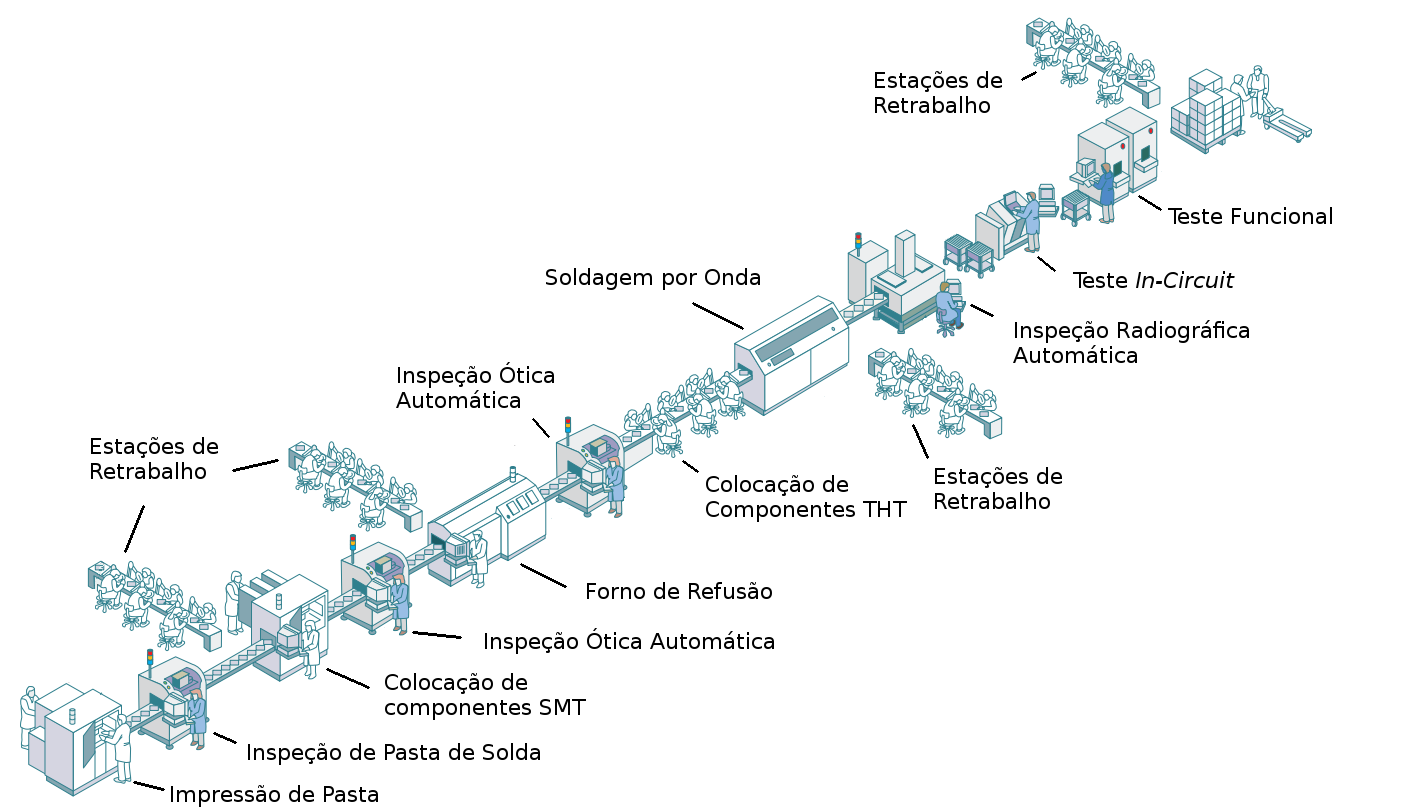
\includegraphics[width=1.1\linewidth]{linha.png}
    \caption{Uma típica linha de montagem de PCIs. Adaptado de \citet{agilenttechnologies2003}}
    \label{fig:linha}
\end{figure}


Juntamente com as métricas de cobertura de teste, os modelos de falta também cumprem um papel importante no estudo de testes de manufatura. \citet{jutman2014high} separa os modelos de falta nas seguintes classes: defeito materiais; defeitos em pinos e malha de circuito; problemas funcionais; e problemas de desempenho. 

Defeitos em materiais e mecânicos podem ser mensurados por métricas padrão de processo de qualidade e exemplificados por defeitos em placas, processo de montagem: solda ruim terminal levantado, componente defeituoso, desalinhamento, efeito lápide\footnote{Efeito Lápide, ou \textit{tumbstone effect}, é a elevação parcial ou total de componentes SMT passivos durante a refusão, assemelhando-se muitas vezes à uma lápide.}.

Os defeitos em pinos e malhas de circuito são modelados por análise estrutural e já possuem uma base bem estabelecida. Entram nessa classe as falhas de circuitos abertos ou em curto, defeito de driver (\textit{buffer}, pino).

Há ainda os problemas \textit{funcionais}, como falhas de \textit{boot}, cujas métricas são estabelecidas e investigadas por pesquisadores em desenvolvimento de software e lógica descritiva.
Por final, tem-se os problemas de desempenho em linhas de comunicação: alta taxa de erro, \textit{crosstalk, jitter, delay,} e outros.

Tradicionalmente na indústria, defeitos em materiais são solucionados durante a montagem da placa. Já os defeitos de pino, malha de circuito e funcional são testados no fim de linha de produção por duas categorias de teste denominados \textit{testes estruturais e testes funcionais}. A relação entre estas duas categorias de testes é descrita em  \citet{thomaswenzelenricozimmermann2016} e sintetizada na figura \ref{fig:cobertura}. Porém, em \citet{thomaswenzel2013} e \citet{jutman2014high}, nota-se que essa segmentação vem mudando com os avanços nas técnicas de verificação periférica e de teste centralizado por microcontrolador, que incorporam boa parte dos testes de desempenho e até mesmo funcionais. Tais técnicas serão descritas nas seção \ref{FCT} deste mesmo capítulo.

\begin{figure}[ht]
    \centering
    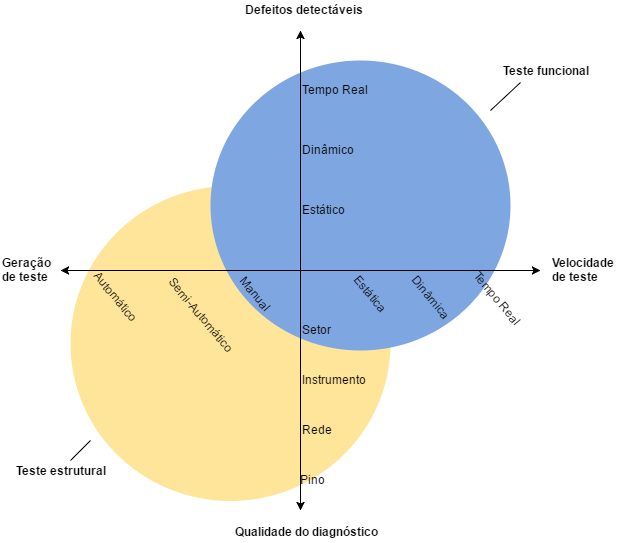
\includegraphics[width=1.0\linewidth]{complement.png}
    \caption{A complementariedade dos testes estruturais e funcionais para a cobertura de teste de um dispositivo. Adaptado de \cite{thomaswenzelenricozimmermann2016}.}
    \label{fig:cobertura}
\end{figure}

Viu-se aqui, portanto, que diversas técnicas e abordagens de teste e diagnóstico integram-se e são parte importante da produção, operação e manutenção de um sistema eletrônico. A seguir, estas técnicas serão descritas detalhadamente. 
\clearpage
\subsection{Inspeção de Pasta de Solda}

A inspeção de pasta de solda é o processo, normalmente automático, de achar falhas após a aplicação da pasta de solda. A inspeção de pasta de solda previne o retrabalho de placas com os componentes montados porque, uma vez com os erros de solda detectados, a placa defeituosa pode ser separada das demais. A detecção de falhas ainda nesta etapa custa 10 vezes menos do que uma falha pós refusão, ou após a solda, e 70 vezes menos que uma falha no teste elétrico intra-circuito (\textit{In-circuit test}) \citep{owen2000process}.

Os sistemas mais simples de inspeção de pasta de solda consistem de uma imagem colorida da placa. Este método consegue detectar ausência de solda e conexões indevidas entre blocos vizinhos, porém, por ser um método 2D, não consegue estimar a altura e volume da pasta de solda. Isso pode gerar problemas indetectáveis em outras etapas, já que, por mais que passe em testes de condutividade, a falta de pasta de solda em uma conexão pode causar problemas mecânicos e rompimento da interconexão. 

O volume de pasta de solda pode ser estimado por diversos métodos. \citet{5246351} introduz as principais tecnologias de perfilometria: 
\begin{itemize}
    \item Triangulação a laser;
    \item Perfilometria por fase, utilizando luz estruturada;
    \item Reconstrução por Redes Neurais.
\end{itemize}

Os métodos por triangulação a laser utilizam-se das projeções do feixe de laser no relevo da placa para reconstruir o seu perfil 3D.  \cite{5576321} descreve os detalhes desta técnica. Medições precisas podem ser obtidas com este método. Entretanto, são equipamentos caros, com baixa velocidade de inspeção, e susceptíveis a ruídos refletivos e \textit{efeito de sombras} \citep{5246351}.

Na perfilometria por fase, uma luz estruturada projeta um padrão, como uma grade ou uma série riscos, na PCI com a pasta de solda aplicada. Este padrão é então pouco a pouco deslocado e uma série de imagens são capturadas por uma câmera de alta resolução. Os sistemas mais avançados empregam um sistema livre de sombras onde ambos os lados da deposição de solda são caracterizados simultaneamente. \cite{5576321} oferece uma abordagem para o problema das sombras e \cite{5246351} faz uma revisão dos principais trabalhos em perfilometria por fase.

O método de reconstrução por redes neurais tenta resolver os problemas do \textit{shape-from-shading (SFS)}, que até então era um método cujo desempenho era inconsistente. \cite{5246351} revisa o estado da arte e propõe uma nova abordagem.

\subsection{Inspeção ótica automática - AOI}
% inserir https://repositorio.ufsc.br/xmlui/bitstream/handle/123456789/158843/337436.pdf?sequence=1&isAllowed=y

A inspeção ótica automática (AOI), como o próprio nome indica, inspeciona visualmente a placa de circuito por meio de fotos, processa e identifica automaticamente as falhas, seja de componente ou solda. Esta técnica é usada para detectar componentes trocados, faltantes ou mal posicionados e pode ser realizada na etapa pré-forno de refusão ou após, dependendo da particularidade do processo produtivo da fábrica. O trabalho de \cite{huang2015automated}, citado por \cite{mello2015sistema}, indica quatro categorias de inspeção ótica automática:

\begin{itemize}
    \item \textbf{Métodos de projeção}, que correlacionam a entrada com modelos aprendidos e suas características;
    \item \textbf{Abordagem baseada em filtro:} filtro espaciais com base em transformadas de sinal, como por exemplo, Fourier, Wavelet, discreta cosseno;
    \item \textbf{Aprendizagem de máquinas:} Os mais utilizados são as redes neurais, algoritmos genéticos, e máquinas de vetor suporte;
    \item \textbf{Abordagens híbridas:} associam diversas técnicas para classificações mais complexas. 
\end{itemize}

%A AOI na etapa pré-forno detecta componentes faltantes ou componentes errados, e alinhamento correto de componentes. Como este processo é realizado após a refusão, os defeitos são relativamente simples de corrigir e menos custosos do que após a etapa de refusão. Outra vantagem é que os problemas de calibração na máquina de posicionamento de componentes podem ser mais facilmente detectados e analisados. Uma análise de tendência nas etapas pós refusão não seria tão confiável, pois o processo de refusão altera a localização dos componentes, e problemas de calibração na máquina de posicionamento só seriam detectados após um aumento significativo de placas defeituosas.

%Na etapa pós refusão, a inspeção ótica automática é provavelmente a etapa mais aceita entre os fabricantes de placas eletrônicas. Um sistema AOI colocado nesta etapa detecta qualquer problema gerado ao longo do processo, incluindo defeitos de colocação de componentes e problemas relacionados à solda, como: falta ou excesso de solda, curto-circuitos ou circuitos abertos. Nesta etapa, a AOI detecta defeitos causados por problemas de impressão, pelo sistema de colocação de componentes, e ainda, pelo processo de refusão. O propósito da AOI após o processo de refusão não é somente prover dados de defeito necessários para o retrabalho de uma PCI, mas também para a coleta de dados através de múltiplas montagens de placa para análise de causa raíz e melhoramento contínuo da produção.

A maior limitação da AOI é a impossibilidade de detecção de defeitos em pinos ou partes do circuito não visíveis, como abaixo de componentes \textit{Ball Grid Array} (BGA) ou em circuitos eletromagneticamente blindados. Nesses casos, é necessário o uso de outras ferramentas, como a verificação de placas por radiografia.
%\cite{savage1993automated} citado por \citep{mello2015sistema}
%todo
\subsection{Inspeção radiográfica automática - AXI}

A inspeção radiográfica automática (AXI) possui uma vantagem única em relação às outras tecnologias de inspeção estrutural: os materiais absorvem os raios-x proporcionalmente à sua massa atômica. A solda utilizada na montagem das PCIs consiste de materiais pesados como o chumbo e a prata. A maioria restante dos materiais usados na fabricação das PCIs é composta por elementos leves como carbono, silício, alumínio, oxigênio, hidrogênio e cobre. Dessa forma, a inspeção radiográfica mostra-se muito interessante na geração de imagens do processo de solda: os pontos de solda aparecem muito bem, enquanto o restante da placa apresenta-se transparente. Outra vantagem é a possibilidade de inspecionar os pinos escondidos de encapsulamentos complexos como o BGA ou o \textit{chip-scale packages} (CSP), além de exibir características internas dos pontos de solda.

\subsubsection{Tipos de AXI}

 As técnicas AXI utilizadas em processos de manufatura e diagnóstico se dividem entre bidimensional e tridimensional \citep{7236817, dougmcclure2000}. 

A inspeção 2D é semelhante à radiografia convencional, porém com recursos de visão computacional para análise automática. É melhor aplicada em placas com soldas em um só lado da placa. Em placas com junções de solda em alta densidade ou em ambos os lados, a imagem gerada pode ficar confusa. 

Com a laminografia e tomografia computadorizada é possível obter a imagem de um recorte da placa e, associada a técnicas de processamento digital, reconstruir um modelo tridimensional da placa. A laminografia utiliza-se do movimento do emissor e detector que pode ser rotacional \citep{7236817} ou linear \citep{6756131}. A desvantagem da radiografia tridimensional é o tempo necessário para a captura da imagem e seu processamento \citep{6756131}. 

\subsubsection{Casos onde a inspeção radiográfica é importante}

\citet{leinbach2001and} apresenta três casos aonde a inspeção radiográfica se faz importante. Primeiro, na inspeção de componentes visualmente ocultos, como terminais de encapsulamentos CSP e BGA ou componentes sob blindagem RF. Segundo, em aplicações que exigem alta qualidade de solda, como as PCI expostas a ambientes de estresse mecânico ou térmico. Terceiro, em projetos de PCI complexos, cujas taxas de erro de produção por placa são mais frequentes e a AXI consegue garantir o rigor do processo de inspeção.

\citet{7236817} faz um estudo comparativo entre tecnologias de inspeção radiográfica para detecção de defeitos em furos galvanizados. \citet{7428398} aplicou AXI na inspeção de componentes \textit{press-fit} e \citet{7428400} na verificação do resinamento de placas de circuito impresso montadas. Combinada com técnicas de ICT, a maior parte dos defeitos podem ser cobertos. O trabalho de \citet{oresjo2002use} comenta melhor a relação entre AOI, AXI, e os testadores intra-circuito (\textit{in-circuit testers - ICT}).

\subsection{Testes intra-circuito (\textit{In-Circuit Testers - ICT)}}

Jigas de teste são uma grande ferramenta de teste de placas de circuitos eletrônicos. Por meio de pontas de teste, pode-se obter acesso a pontos internos do circuito, como também, testar componentes isoladamente, separando-os de outros circuitos. Por meio de ICT, é possível detectar componentes defeituosos ou faltantes, circuitos abertos ou em curto e, até mesmo, componentes errados. O ICT trabalha testando partes isoladas da placa, medindo resistência, capacitância e, em alguns casos, indutância de subcircuitos da placa, normalmente acessíveis por conectores, pads, ou \textit{test points}. Dessa forma, consegue-se realizar testes estruturais e até mesmo funcionais sobre o circuito, garantindo que sua fabricação foi correta e que se encontra funcional. Muitas vezes, o ICT é usado também para a gravação de \textit{firmware} nas placas. Os ICT são compostos pelos seguintes elementos \citep{ianpoole2017}:

\begin{itemize}
    \item O ICT em si: composto por uma matriz de pares de acionadores e sensores que são usados para realizar as medições. Podem ser em torno de centenas, ou até milhares, por ICT.
    \item A jiga de teste (\textit{fixture} ou fixação):  é a interface entre o ICT e a placa testada, roteando as entradas e saídas do ICT com o Dispositivo em Teste, através de pinos, num arranjo conhecido como cama de pregos.
    \item O software de teste: software com a rotina de testes e condições de aprovação/reprovação.
\end{itemize}

Dentre os três, somente o ICT em si não é customizado para cada placa. O sistema de jiga de testes, por ser relativamente caro, é mais bem aplicado a grandes volumes de produção. Uma análise de custos deve de ser realizada para garantir que os custos de montagem da jiga e do programa sejam viáveis. 

\subsubsection{Tipos de ICT}

A tabela \ref{table:tiposdeict} sintetiza três categorias principais de testadores \citep{ianpoole2017}: O ICT tradicional; O \textit{flying probe test - FPT}, cujas pontas de prova são controladas por comando numérico computadorizado (CNC); e o Analisador de Defeito de Fabricação: versão mais enxuta do ICT, com funcionalidades reduzidas. 

\begin{table}[h!]
\centering
\caption{Tipos de ICT}
\label{table:tiposdeict}
{\footnotesize 
\begin{tabularx}{\textwidth}{@{} Y Y Y Y @{}}
\toprule
  \textbf{Tipo de ICT} & \textbf{Princípio de \mbox{Funcionamento}}  &\textbf{Vantagens}  &\textbf{Desvantagens} & \\ \midrule
\textbf{ICT tradicional} & - Pares de I/O em grande número; 

- Fixação e cama de pregos feitos sob medida. & - Alta velocidade de execução de teste; 

- Capacidade para medição de capacitância e indutância. & - Inviável para pequenas produções;

- Custo adicional para qualquer atualização da jiga;  \\ \addlinespace
\textit{\textbf{Flying probe test (FPT)}} & - Pontas de prova móveis e controladas por CNC; 

- A fixação de placa é genérica;
 & - Dispensa uma jiga de teste e cama de pregos; 
 
 - Alterações realizadas via software;
 & 
- Número limitado de pontos de testes simultâneos; 

- Baixa velocidade de teste; & \\ \addlinespace
\textbf{Analisador de Defeitos de Fabricação}
 & - Similiar ao ICT padrão, mas com funções limitadas.
 & - Alta velocidade de teste e custo reduzido;
 & - Limita-se a testes de continuidade e resistência elétrica.
  & \\ \bottomrule
\end{tabularx}}
\end{table}

\subsubsection{Cobertura de falta}
Em sua tese, \citet{de2008apoio} relata que os testes funcionais e estruturais realizados por ICT foram progressivamente dificultados por duas questões. 

A primeira é a miniaturização dos circuitos e componentes com valores muito baixos, cuja verificação é comprometida  devido à influência de capacitâncias parasitas do próprio testador. O mesmo acontece com as indutâncias mas, ao menos, é possível detectar a presença do componente ao medir a resistência entre os terminais.

O segundo problema, e também o mais grave, é relacionado ao acesso aos nós do circuito, seja pelas dimensões reduzidas da placa sob teste, que dificultam a construção de uma cama de pregos correspondente, como também pela completa inacessibilidade a uma região eletromagneticamente blindada ou a pinos inacessíveis de encapsulamentos de alta densidade, como os BGAs, que, hoje em dia, estão quase sempre presentes em placas de circuito impresso.

Estes fatores deram origem ao desenvolvimento da infra-estrutura normatizada de circuitos de varredura periférica IEEE 1149.1 \citep{ieee11491old} para facilitar o teste de integrados digitais que, nas ultimas décadas, expandiu-se em outros padrões que cobrem desde medições analógicas a testes de canais de comunicação. 

\subsection{Varredura periférica}

Testes de varredura periférica (\textit{boundary scan}) como o \textit{Joint Test Action Group - JTAG} são hoje o padrão da indústria em teste de placas de circuito impresso e vem, ao longo dos últimos anos, substituindo os ICT. Isso se deve ao custo baixo desta tecnologia e eficiência em termos de cobertura de testes. Os primeiros esforços para a criação de um padrão de varredura periférica ocorreram na década de 80 e foram encabeçados pelo \textit{Joint Test Action Group - JTAG}, cujo trabalho se consolidou no padrão \citet{ieee11491old}, que obteve rápida adoção pela indústria eletrônica. Sua revisão mais atual é a \citet{ieee11491yr2013}.
A necessidade de um padrão de varredura periférica surgiu devido aos crescentes custos e dificuldades na criação de jigas de teste para ICTs, principalmente pelo aumento da densidade de componentes e pela falta de espaço para a inserção de pontos de teste no leiaute de circuito impresso, como também, por causa da distribuição de componentes em ambas as superfícies. 

Embora as primeiras aplicações do JTAG fossem direcionadas para teste de placas de circuito impresso, hoje o padrão também cumpre um papel essencial na depuração de sistemas embarcados, graças ao acesso de baixo nível às entradas/saídas e estados internos do circuito integrado, fornecendo um meio barato e confiável de depuração.
A porta JTAG também serve para a gravação de \textit{firmware} na memória flash \citep{ieee1532}, sendo uma alternativa mais rápida ao uso de portas seriais e \textit{bootloaders}. 

Outra aplicação desta interface é a geração de testes automatizados para diagnóstico de placa em campo no conceito de BIST, ou auto teste embutido, possibilitando que uma placa faça auto-diagnóstico de problemas, como em circuitos periféricos. Estes conceitos serão abordados no próxima seção deste trabalho.

\begin{figure}
    \centering
        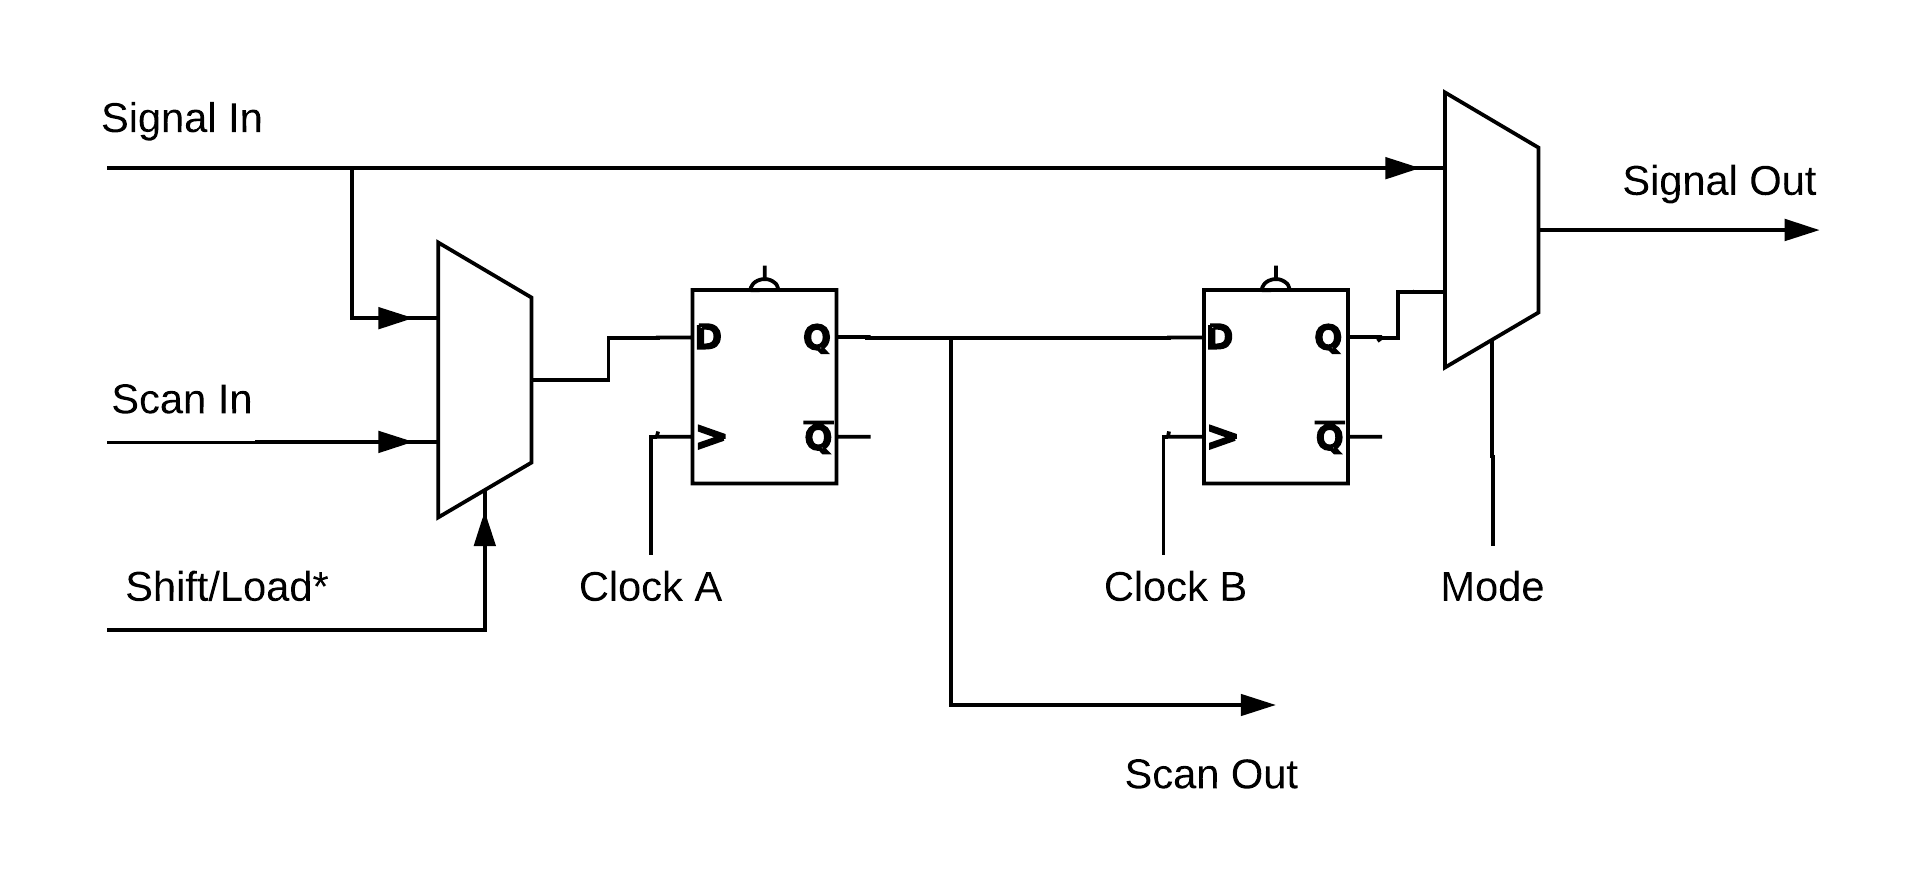
\includegraphics[width=0.8\linewidth]{fig/bscell}
            \caption{Célula de Verificação Periférica}
            \label{fig:bscell}
\end{figure}


O padrão IEEE 1149.1 se baseia em células de teste embutidas em todos os pinos de E/S do circuito integrado (figura \ref{fig:bscell}). As células são encadeadas em uma topologia em anel, um esquema conhecido como \textit{daisy-chain}. O gerenciamento da cadeia de verificação é realizado pela porta de acesso ao teste (ou, em inglês, \textit{test acess port - TAP}), permitindo que todos os pinos de E/S do circuito integrado sejam acessíveis e testados pela porta JTAG. A figura \ref{fig:tap} mostra o esquemático conceitual da lógica interna da porta JTAG. A conexão em \textit{daisy-chain} entre os pinos de um dispositivo com suporte ao IEEE 1149.1 pode facilmente ser estendida para outros integrados compatíveis com o padrão, possibilitando o teste de múltiplos circuitos integrados através de um único conector (figura \ref{fig:cadeiabs}). Como boa prática de DfM, recomenda-se a escolha de integrados que atendam ao padrão.

\begin{figure}
    \centering
        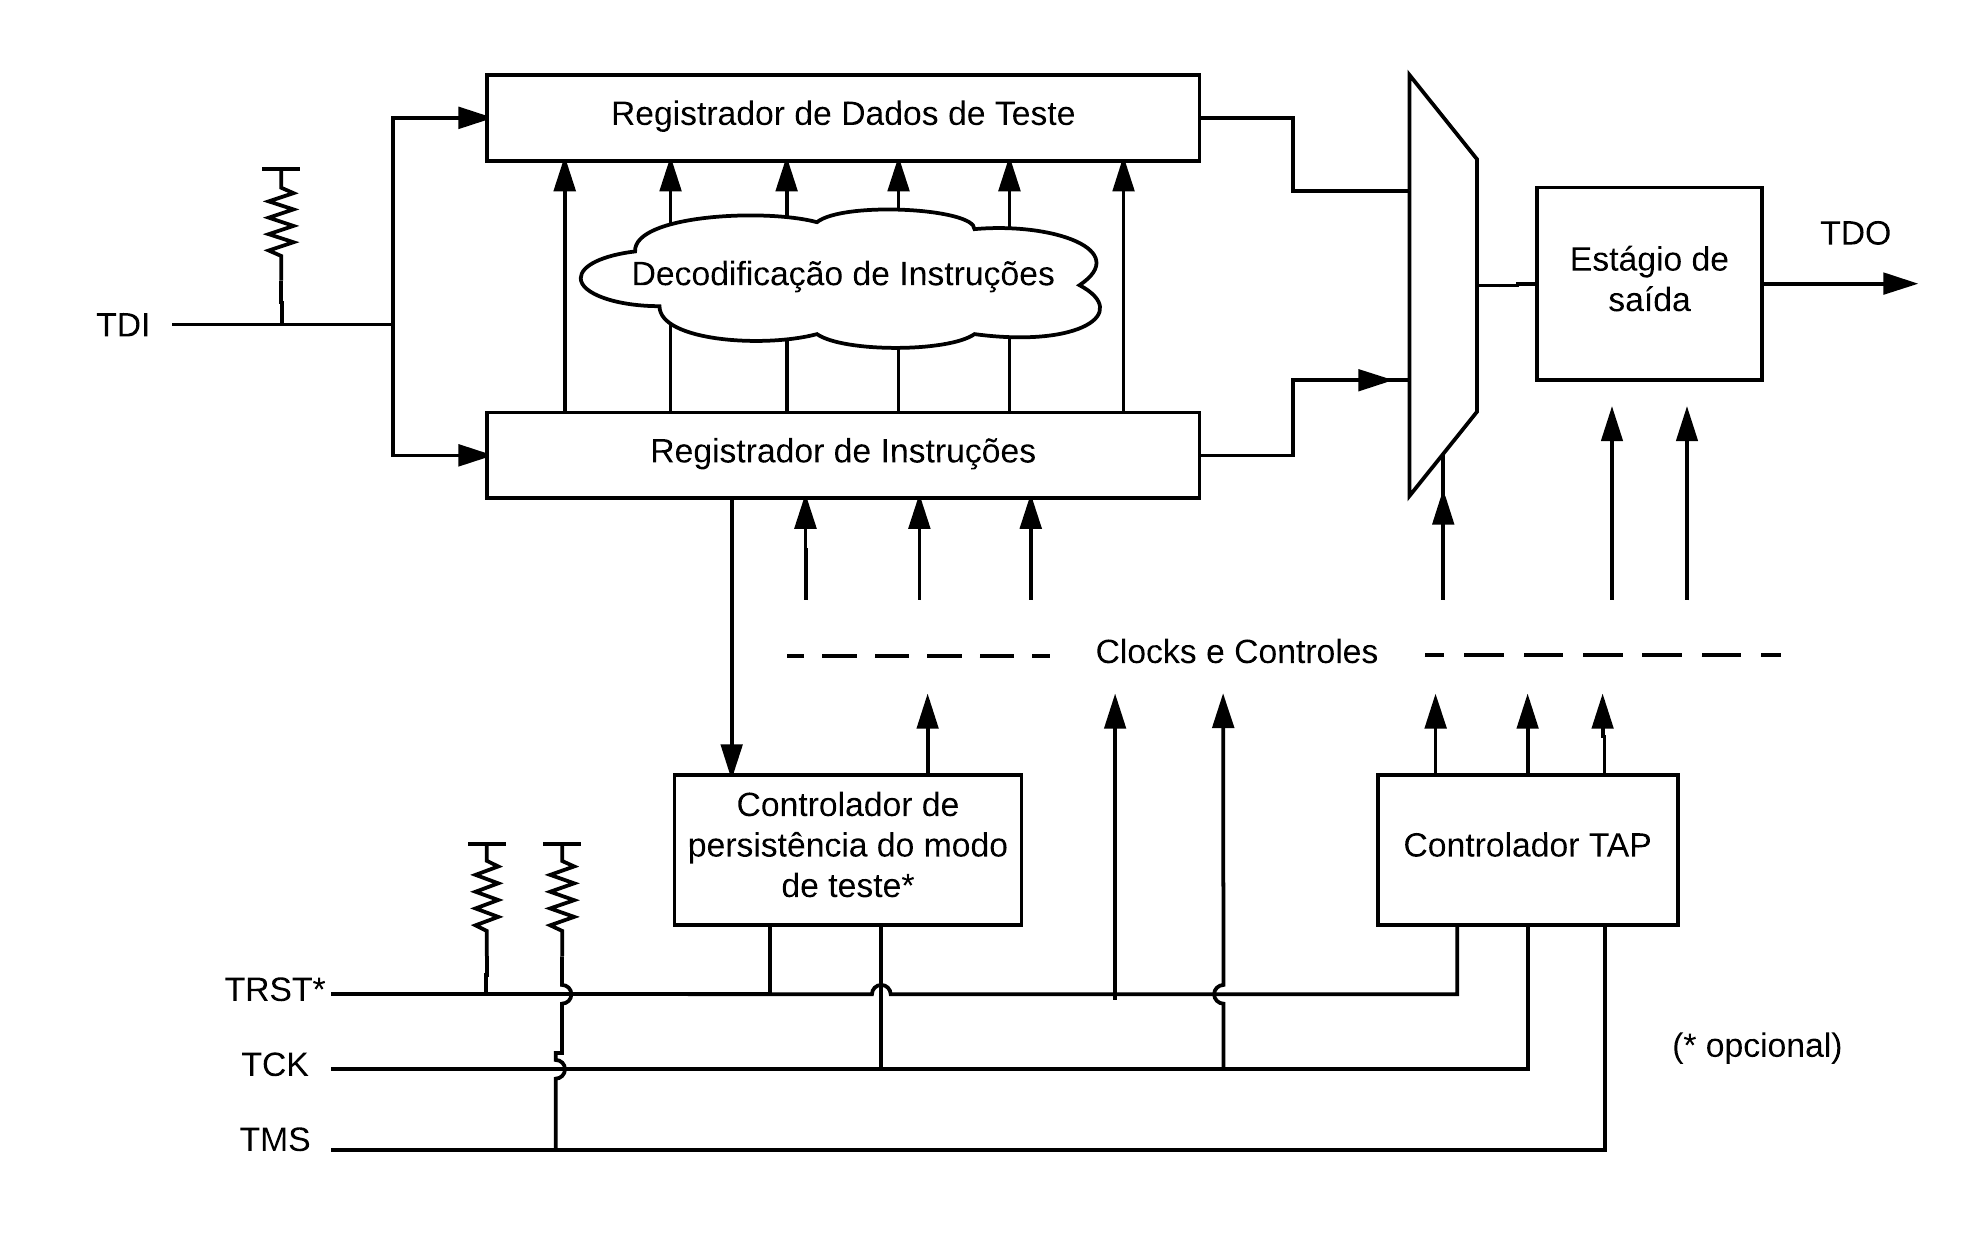
\includegraphics[width=1.0\linewidth]{fig/TAP}
            \caption{Esquemático conceitual da lógica de teste \textit{on-chip}}
            \label{fig:tap}
\end{figure}

Outro componente importante do JTAG é a linguagem de descrição de varredura periférica (BSDL em inglês), que foi inserida numa revisão posterior do IEEE 1149.1 \citep{ieee11491de94}. A BSDL é um subconjunto do VHDL e é voltada para a descrição da infraestrutura de teste de um CI com o objetivo de tornar mais consistente a geração de testes e toda a cadeia de desenvolvimento envolvida nisso.

\begin{figure}
    \centering
        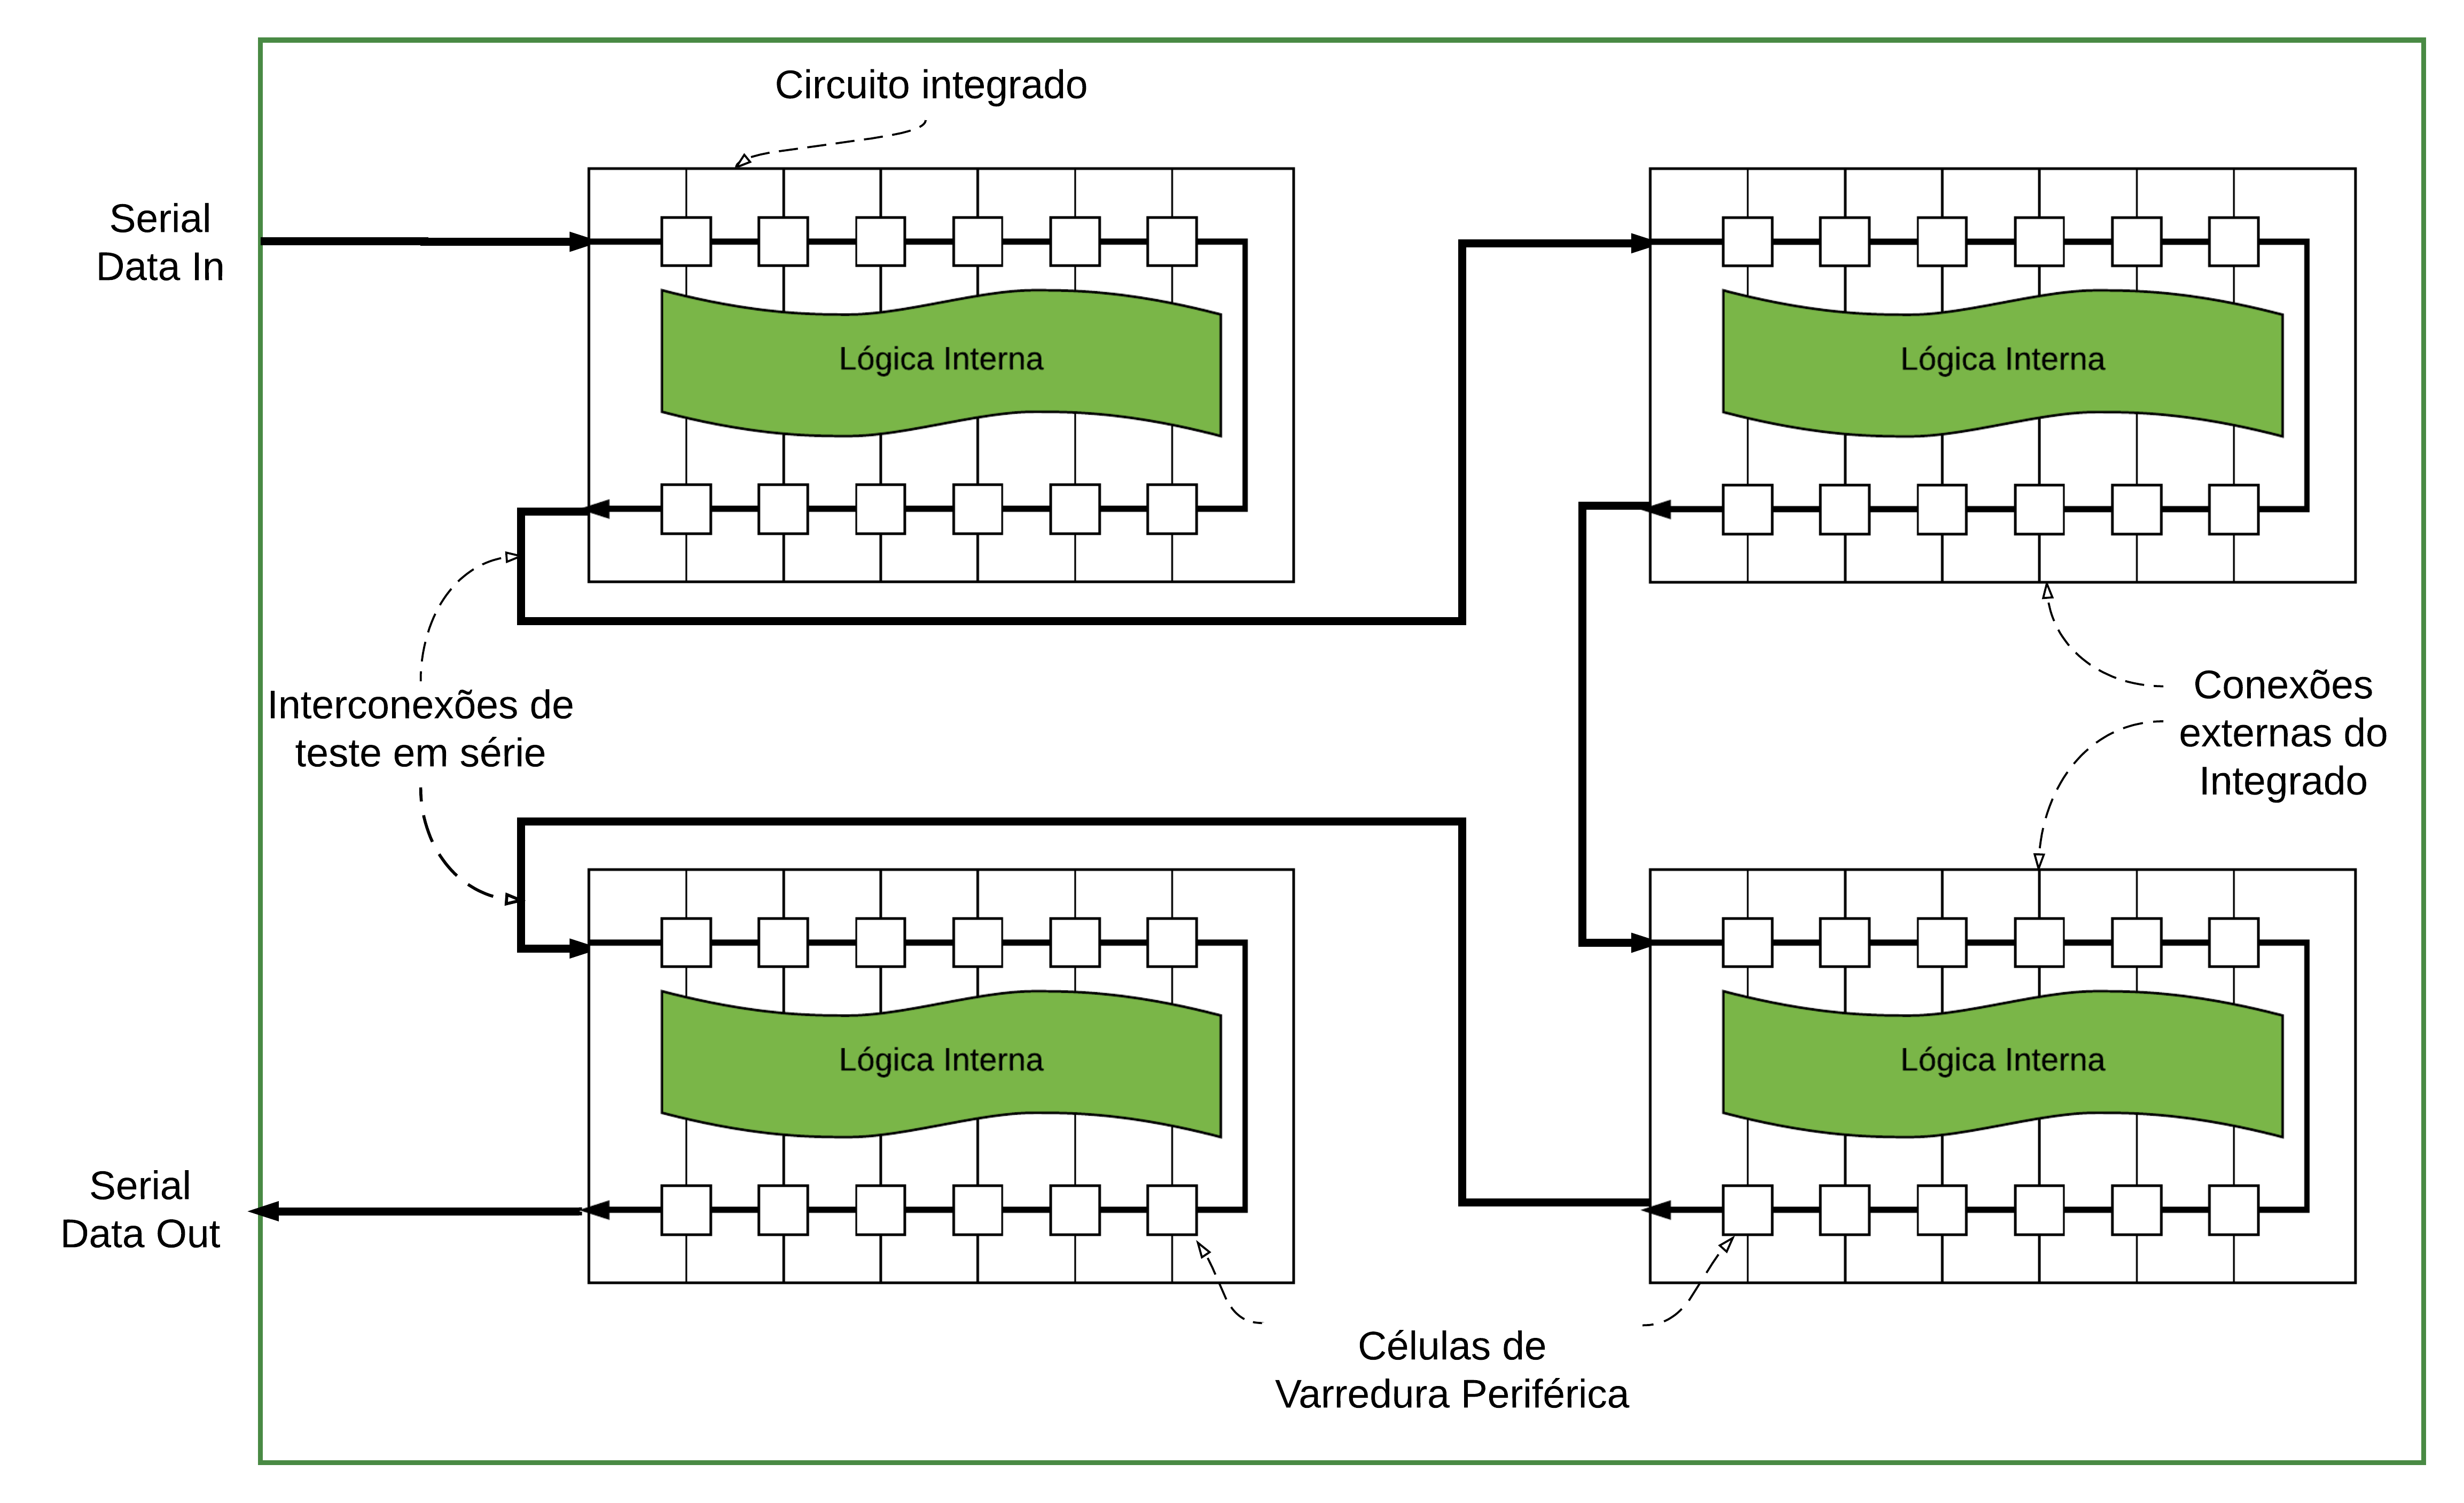
\includegraphics[width=1.0\linewidth]{fig/cadeiabs}
            \caption{PCI com as portas JTAG em \textit{daisy-chain}}
            \label{fig:cadeiabs}
\end{figure}


O padrão IEEE 1149.1 serviu de base para a criação de uma família de padrões de varredura periférica, que são exibidos na tabela \ref{tab:boundaryscanfamily} - adaptada de \citet{jutman2014high}.  

\begin{table}[h]
\centering
\tiny
\caption{Padrões IEEE de varredura periférica \citep{jutman2014high}}
\label{tab:boundaryscanfamily}
\begin{tabular}{p{50}p{50}p{50}p{50}}
\hline
\rowcolor[HTML]{C0C0C0} 
\multicolumn{1}{|p{50pt}|}{\cellcolor[HTML]{C0C0C0}\textbf{Foco principal de aplicação}} & \multicolumn{1}{p{50pt}|}{\cellcolor[HTML]{C0C0C0}\textbf{Propósito Principal}} & \multicolumn{1}{p{50pt}|}{\cellcolor[HTML]{C0C0C0}\textbf{Base da Tecnologia}}    & \multicolumn{1}{p{50pt}|}{\cellcolor[HTML]{C0C0C0}\textbf{Classes de falta a serem cobertas}}     \\
\rowcolor[HTML]{656565} 
\multicolumn{4}{|l|}{\cellcolor[HTML]{656565}{\color[HTML]{FFFFFF} \textbf{IEEE 1149.1 - Boundary Scan \citep{ieee11491old, ieee11491yr2013}}}}                                                                                        \\
\multicolumn{1}{|p{50pt}|}{Teste de Manufatura de PCI}                                        & \multicolumn{1}{p{50pt}|}{Melhorias de acesso aos testes}                               & \multicolumn{1}{p{50pt}|}{Registradores de sondagem on-chip}                            & \multicolumn{1}{p{50pt}|}{Faltas em pinos e integridade de circuto}                                 \\
\rowcolor[HTML]{656565} 
\multicolumn{4}{|l|}{\cellcolor[HTML]{656565}{\color[HTML]{FFFFFF} \textbf{IEEE 1149.4 - Barramento para testes de sinais mistos \citep{ieee11494}}}}\\

\multicolumn{1}{|p{50pt}|}{Medição de sinais analógicos} &
\multicolumn{1}{p{50pt}|}{Melhorias de acesso aos testes} & 
\multicolumn{1}{p{50pt}|}{Chaves \textit{on-chip}} &
\multicolumn{1}{p{50pt}|}{Valores paramétricos}\\

\rowcolor[HTML]{656565} 
\multicolumn{4}{|l|}{\cellcolor[HTML]{656565}{\color[HTML]{FFFFFF} \textbf{IEEE 1149.6 - Teste BST de Redes Digitais Avançadas \citep{ieee11496}}}}\\

\multicolumn{1}{|p{50pt}|}{Teste de redes LVDS de alta velocidade} &
\multicolumn{1}{p{50pt}|}{Teste de malhas acopladas em corrente alternada} & 
\multicolumn{1}{p{50pt}|}{Geradores de pulsos \textit{on-chip}} &
\multicolumn{1}{p{50pt}|}{integridade de malha}\\

%\rowcolor[HTML]{656565} 
\multicolumn{4}{|l|}{\cellcolor[HTML]{656565}{\color[HTML]{FFFFFF} \textbf{IEEE 1149.7 - Pinos reduzidos e TAP aprimorado \citep{ieee11497}}}}\\

\multicolumn{1}{|p{50pt}|}{Teste de placa e depuração de software} &
\multicolumn{1}{p{50pt}|}{Acesso à teste flexivel e em alta velocidade por dois pinos} & 
\multicolumn{1}{p{50pt}|}{SERDES, endereçamento} &
\multicolumn{1}{p{50pt}|}{Contempla todos acima}\\

%\rowcolor[HTML]{656565} 
\multicolumn{4}{|l|}{\cellcolor[HTML]{656565}{\color[HTML]{FFFFFF} \textbf{IEEE 1149.8.1 - Alternância de pinos e sensoriamento sem contato\citep{ieee114981}}}}\\

\multicolumn{1}{|p{50pt}|}{Teste de interconexão de PCIM} &
\multicolumn{1}{p{50pt}|}{Ligações para componentes passivos} & 
\multicolumn{1}{p{50pt}|}{chapas de sensoriamento capacitivo} &
\multicolumn{1}{p{50pt}|}{Circuitos abertos: AC e DC }\\

\multicolumn{4}{|l|}{\cellcolor[HTML]{656565}{\color[HTML]{FFFFFF} \textbf{IEEE P1149.10- TAP de alta velocidade \citep{ieeep1149102016} }}}\\

\multicolumn{1}{|p{50pt}|}{O mesmo que todos acima} &
\multicolumn{1}{p{50pt}|}{Permutação de dados de teste em alta velocidade} & 
\multicolumn{1}{p{50pt}|}{Reuso de pinos I/O de alta velocidade} &
\multicolumn{1}{p{50pt}|}{O mesmo que todos acima}\\

\multicolumn{4}{|l|}{\cellcolor[HTML]{656565}{\color[HTML]{FFFFFF} \textbf{IEEE 1500 - Teste de núcleo embarcado \citep{ieee1500}}}}\\

\multicolumn{1}{|p{50pt}|}{Teste à nível de SoC e IP} &
\multicolumn{1}{p{50pt}|}{Acesso ao teste de \textit{IP cores} em um SoC} & 
\multicolumn{1}{p{50pt}|}{invólucros de núcleos} &
\multicolumn{1}{p{50pt}|}{Faltas no domínio digital dentro de um CI}\\

\multicolumn{4}{|l|}{\cellcolor[HTML]{656565}{\color[HTML]{FFFFFF} \textbf{IEEE 1687 - Acesso por Instrumentação Embarcada \citep{ieee1687}}}}\\

\multicolumn{1}{|p{50pt}|}{Teste de CI, depuração, diagnóstico} &
\multicolumn{1}{p{50pt}|}{Padrão de acesso por instrumento} & 
\multicolumn{1}{p{50pt}|}{Cadeias de sonda reconfiguráveis} &
\multicolumn{1}{p{50pt}|}{Específicas do instrumento}\\

\multicolumn{4}{|l|}{\cellcolor[HTML]{656565}{\color[HTML]{FFFFFF} \textbf{IEEE P1838 - Acesso a teste para CIs 3D \citep{ieeep18382016}}}}\\

\multicolumn{1}{|p{50pt}|}{Teste de integração 3DSIC} &
\multicolumn{1}{p{50pt}|}{Acesso à teste através das vias TSV} & 
\multicolumn{1}{p{50pt}|}{O mesmo que os padrões 1500, 1149.1, 1687} &
\multicolumn{1}{p{50pt}|}{Integridade das vias TSV}\\
\hline


\end{tabular}
\end{table}

O padrão IEEE 1149.4 \citep{ieee11494} foi criado para testes paramétricos de componentes passivos, resistores pull-ups, componentes ativos como diodos, transistores e de redes de impedância. Serve como uma extensão da varredura periférica para sinais analógicos. Este padrão ainda tem um número limitado de dispositivos compatíveis.

Já o padrão IEEE1149.6 \citep{ieee11496} estende a varredura periférica a portas de comunicação com acoplamento em corrente alternada, como por exemplo, portas que atendem ao padrão de LVDS, operando em paralelo com os padrões 1149.1 e 1149.4. O que possibilita esta tecnologia são as inserções de geradores de pulso nos pinos de saída e \textit{receivers} CA comuns e diferenciais nas entradas dos dispositivos que dão suporte a este padrão.

É possível citar outros exemplos significativos, como é o caso do IEEE1149.7 - cJTAG \citep{ieee11497}. Este padrão opera em pinos reduzidos e possibilita uma topologia em estrela ao invés do \textit{daisy-chain}, permitindo um acesso mais rápido, além de oferecer uma infraestrutura adicional de suporte a tecnologias mais avançadas. O IEEE P1687 \citep{ieee1687} introduz o conceito de instrumentação embarcada para a aplicação de tarefas de teste, medição e diagnóstico, assunto abordado na próxima seção.

\subsection{Teste Controlado por FPGA ou Processador e Instrumentação Embarcada}
\label{FCT}

Conforme mencionado anteriormente, o JTAG não permite o uso de padrões de teste em velocidade nominal, deixando a classe de falhas de desempenho sob responsabilidade de testes funcionais. Atualmente, parte da indústria tem utilizado os componentes centrais de seus sistemas, como por exemplo os FPGAs e microcontroladores, como dispositivos de teste embarcado \citep{alcrouch2011, thomaswenzel2013}, cunhando os termos \textit{FPGA-Controlled Test - FCT} e \textit{Processor-Controlled Test - PCT}. 

 Além de cobrir os testes em domínio CA, como atrasos e \textit{crosstalk}, ainda possibilitam um acesso de baixo nível no sistema, já que esses são normalmente componentes centrais do projeto. O custo marginal é ínfimo, já que o todo o hardware de teste é reutilizado do produto e a memória de teste é apagada, voltando o dispositivo para sua funcionalidade original. \citet{jutman2014high} afirmou que ainda são poucas as empresas que fornecem ferramentas automatizadas para esta classe de testes.

O conceito de teste controlado por FPGA é possibilitado pelo uso de instrumentos embarcados, que são definidos como qualquer estrutura lógica dentro de um dispositivo cuja função é de teste, diagnóstico, \textit{Design for Testability (DfT), Design for Debug  (DfD), Design for Yield (DfY),} e outros. Neste escopo, enquadram-se diversas estruturas lógicas:    
\begin{itemize}
    \item Testadores de memória e BIST/BISD;
    \item Analisadores de taxa de erro (BERT) em canais de comunicação;
    \item Geradores de padrões de teste e \textit{buffers} de captura digital;
    \item Caracterizadores e Calibradores de E/S complexas;
    \item Testadores de barramentos de comunicação LAN, SATA, PCI, CAN, LIN, I2C, SPI e UART;
    \item Testadores sistêmicos e programação de memórias não voláteis;
    \item Instrumentos definidos por usuário.
\end{itemize}

\citet{Stollon2011} mostra que estas estruturas de instrumentação embutida surgiram, em parte, pela necessidade de medições que causem menos interferências ou que não comprometam a integridade do sinal de barramentos de alta velocidade, internos ou externos ao CI. Dessa forma, os fabricantes passaram a embutir núcleos de propriedade intelectual - \textit{IP cores} - de instrumentação interna, permitindo testes não intrusivos e facilitando a validação e diagnóstico de placas.

Originalmente, cada um destes instrumentos são acessados e gerenciados por uma variedade de instrumentos externos, usando diversos mecanismos e protocolos. Isso dificulta a integração entre CIs e o reuso de tecnologia e equipamento. Logo, existia uma necessidade de padronização destes protocolos, de forma a garantir uma metodologia eficiente e organizada para a preparação de testes e para o acesso e controle destes instrumentos embarcados. 

O IEEE 1687 \citep{ieee1687}, também conhecido como \textit{Internal JTAG } ou IJAG, foi o padrão criado para definir e descrever as interfaces de acesso à instrumentação embarcada pela porta padrão IEEE1149.1, possibilitando a realização de testes avançados e não intrusivos em uma PCI inteira pela porta JTAG. Como ilustrado na figura \ref{fig:ieee1687}, o IJTAG não define os instrumentos ou suas funcionalidades por si, mas sim os padrões de infraestrutura de acesso e como descrever os métodos e funcionalidades dos instrumentos. Isso se consolidou em duas linguagens de descrição dentro deste padrão: uma para as características destas funcionalidades, a PDL \textit{(procedural description language)}, e outra para os requerimentos de interface com estas funcionalidades - ICL \textit{(instrument connectivity language)}. Estas duas linguagens de descrição - PDL e ICL - facilitam o reuso e a descoberta de qualquer instrumento que seja compatível com o padrão IEEE 1687, independente do seu tipo, propósito ou origem. 

\begin{figure}
    \centering
        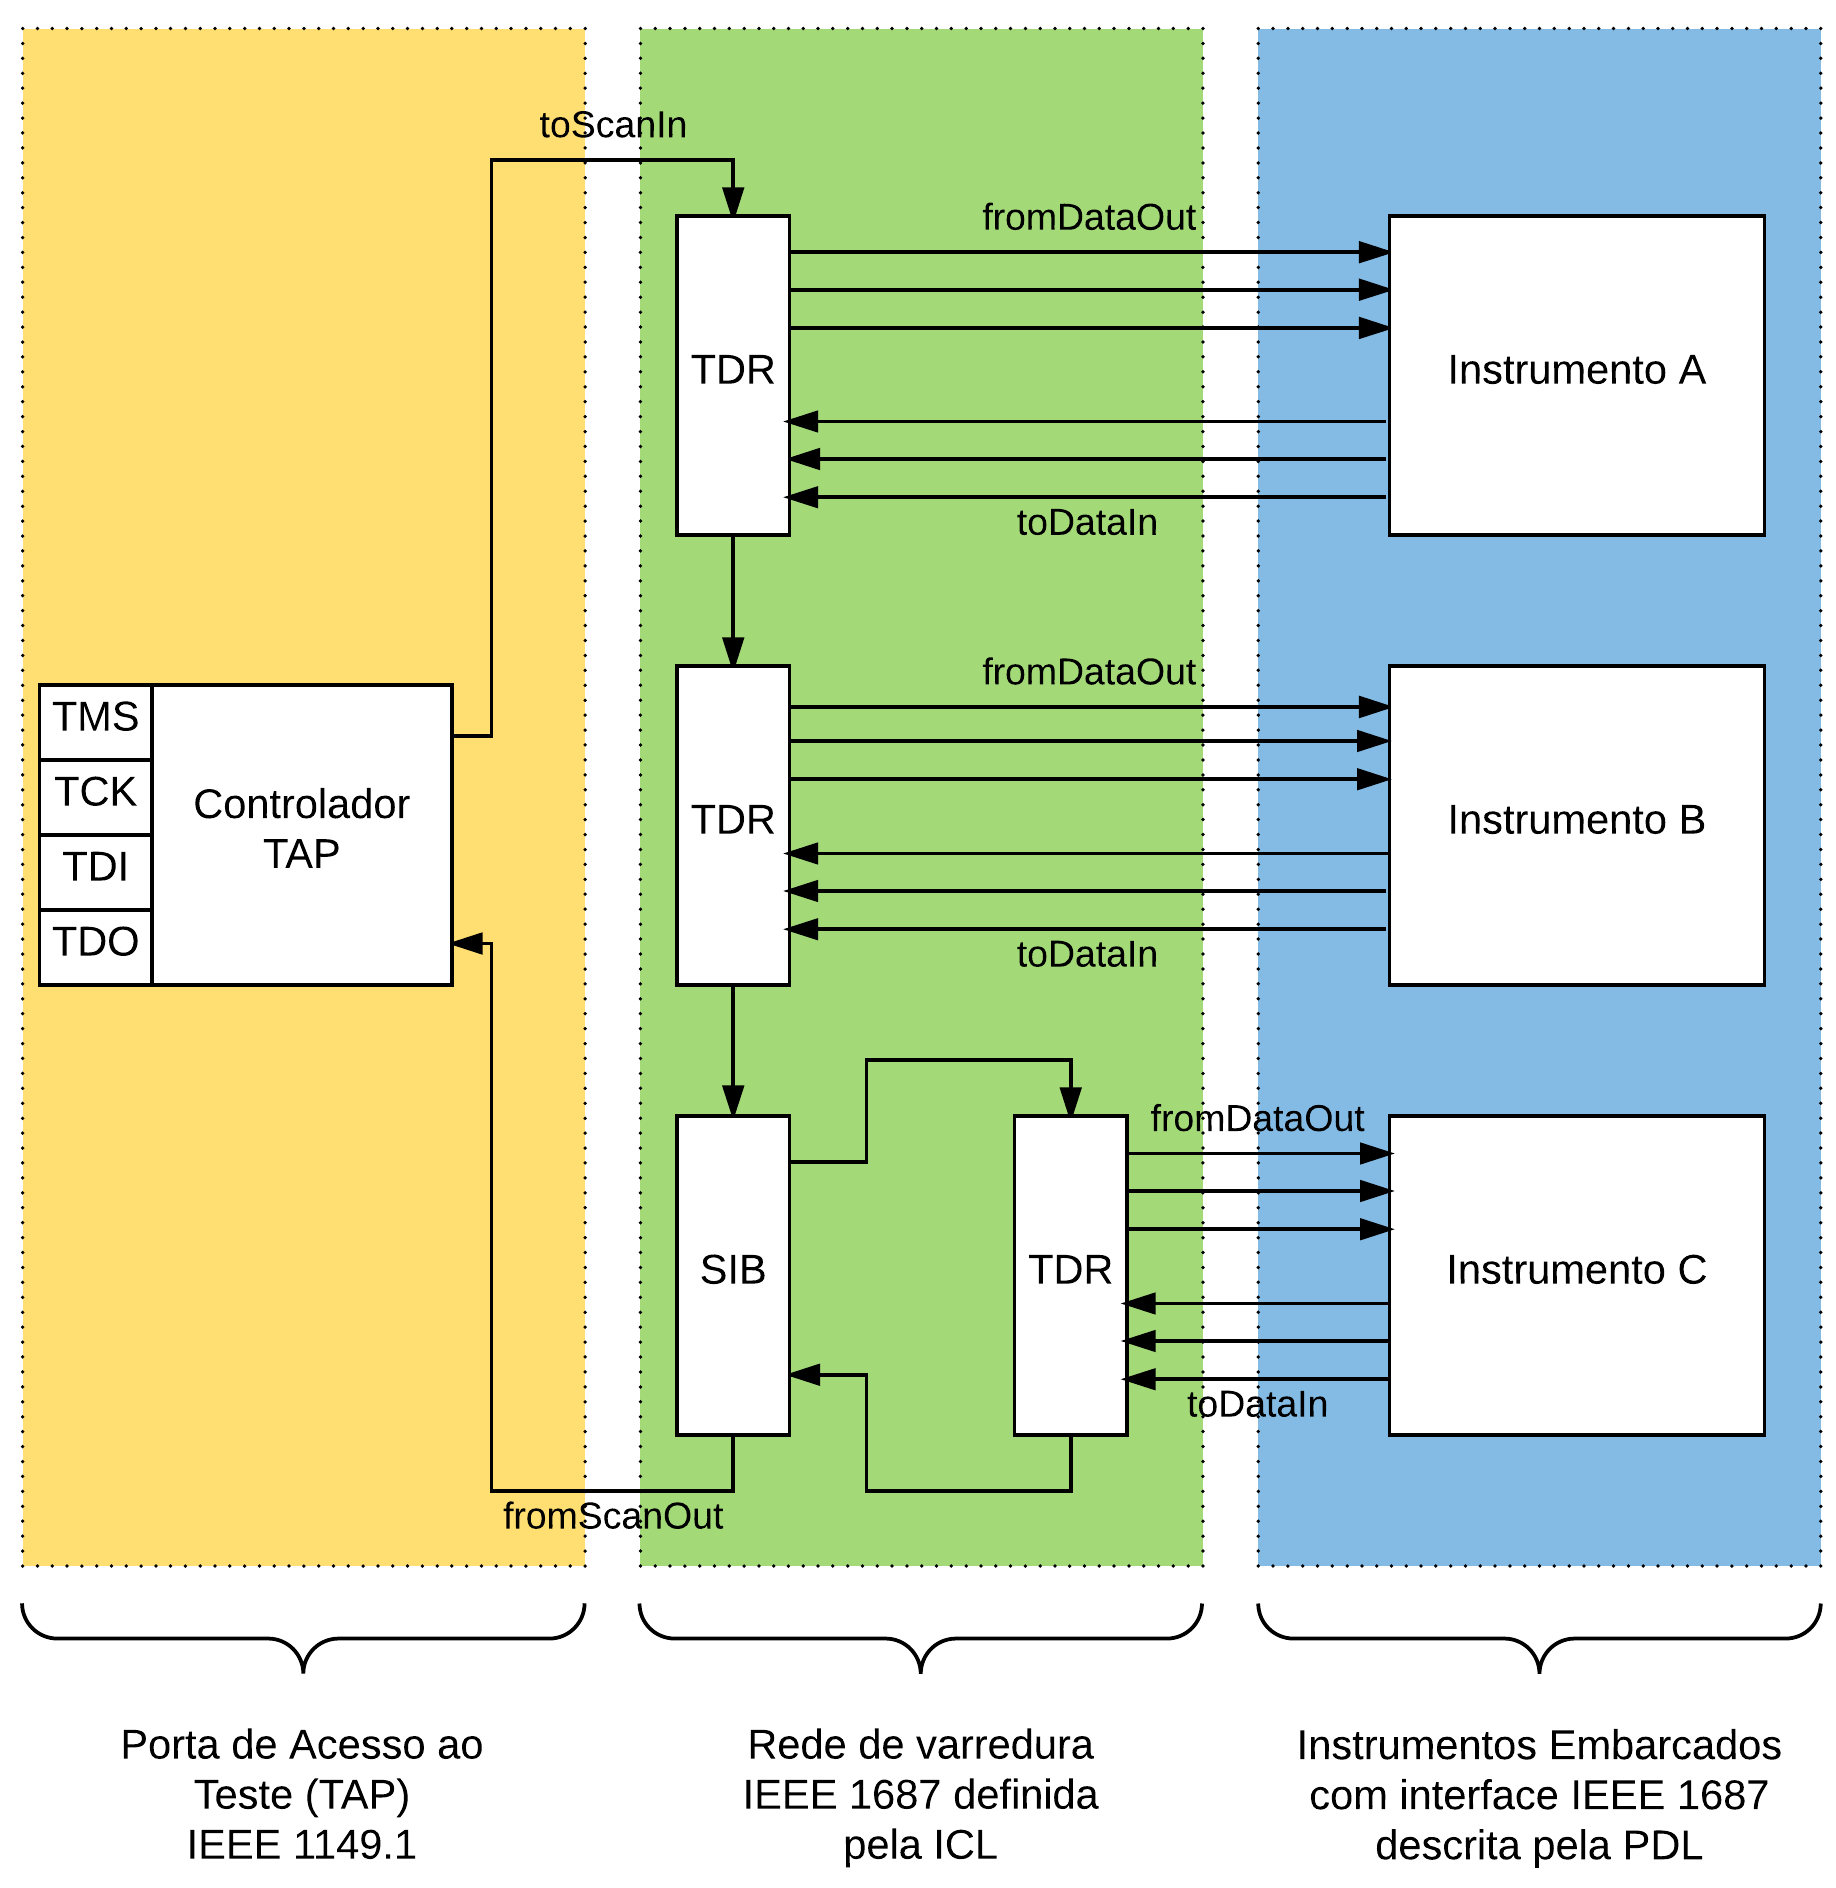
\includegraphics[width=1.0\linewidth]{fig/IEEE1687}
            \caption{Rede IEEE 1687 conceitual de múltiplas cadeias de varredura}
            \label{fig:ieee1687}
\end{figure}

Dessa forma, o padrão IEEE 1687 funciona como uma extensão do IEEE 1149.1, de maneira que a porta JTAG de um CI ou uma placa possa ser usada para configurar, operar, e coletar dados de instrumentos embarcados.

Os FCT e PCT aliados ao IEEE 1687 oferecem uma cobertura em múltiplos domínios de falta (estruturais, CC, CA e faltas de desempenho), reduzindo ou até mesmo superando a necessidade de equipamentos de teste especializados \citep{thomaswenzel2013}. Em \citet{jutman2014high} observa-se que isso possibilita não só uma manufatura e teste de produção mais baratos e descomplicados, como também abre porta para o reuso dos testes em campo para o diagnóstico de falhas operacionais, o que não só reduz os custos logísticos de transporte de equipamentos especializados para depuração e diagnóstico, como possibilita que testes avançados sejam realizados sob condições reais de operação. 

\subsection{Teste Funcional}
% https://pad.riseup.net/p/RwPsE9imTtNzadskjasdoqidjefkadf
%definição
Define-se teste funcional como aquele que não depende da estrutura interna de DfT de um sistema, mas sim das portas de entrada e saída \citep{jutman2014high}. Outra definição, formulada pelo mesmo autor, é a de um teste que se baseia somente nas informações funcionais do sistema, sem conhecimento da estrutura interna. Essas duas definições se interseccionam na maioria das vezes.

% APLICAÇÕES
% quero dizer que em todos autores é unanime que
O teste funcional serve para complementar objetivos específicos de teste, sendo normalmente empregado como etapa final de linha de produção \citep{thibeault2006,jutman2014high,tumim2001}. A tendência é que o teste funcional, devido aos seus custos crescentes, perca espaço com a adesão e popularização dos padrões mais avançados de varredura periférica e instrumentação embarcada, limitando-se a atingir certos objetivos específicos de teste que não podem ser cobertos por testes de varredura \citep{thibeault2006, thomaswenzelenricozimmermann2016}. 

Entretanto, existem casos onde o suporte ao IEEE 1149.1 é inexistente e o teste funcional é a única opção para validação do produto. \citet{tumim2001} afirma que, mesmo com os últimos avanços nos testes de varredura periférica, o teste funcional ainda é insubstituível. Vale lembrar da relação complementar entre essas duas categorias de teste, ilustrada pela figura \ref{fig:cobertura}. 

\citet{jutman2014high} elenca outras aplicações de testes funcionais, dentre elas: a inspeção de recebimento de componentes de terceiros (por exemplo: uma fonte de alimentação feita por outro fabricante, ou circuito integrado de alto valor) e em casos de teste em campo do circuito eletrônico, quando se depende de equipamento externo especializado para a realização de testes ou o fabricante original do CI não disponibiliza o acesso à infraestrutura de teste interna.

%vantagens e desvantagens reescrever
%\citet{thibeault2006} enumera algumas das principais vantagens e desvantagens do teste funcional, destacando-se: 

Destacam-se dentre as principais vantagens do teste funcional:
\begin{itemize}
    \item A possibilidade de execução de testes em velocidade nominal de operação, possibilitando a detecção de defeitos relacionados a temporização \citep{thibeault2006};  
    \item Verificações funcionais que garantam que o projeto opera como prometido,  coisa que testes estruturais e de varredura não conseguem fazer \citep{tumim2001}.
\end{itemize}

Já entre as desvantagens: 

\begin{itemize}
    \item O processo de teste funcional em velocidade nominal é muito mais demorado, se comparado com a varredura periférica \citep{thibeault2006}; 
    \item O esforço e o tempo requerido para gerá-los podem ser significativos e a dificuldade cresce exponencialmente em relação ao número de portas lógicas. Essa dificuldade persiste ainda que existam algoritmos para o teste funcional das estruturas lógicas mais comuns, como CPUs, MMUs, BPU, processadores multicores e GPUs.
\end{itemize}
 
%o que compõe
Como um sistema caixa preta, o teste funcional é composto por dados de excitação, a saída resultante do teste e também um roteiro de teste. Em abordagens tradicionais, o teste funcional de interfaces com periféricos e interconexões é gerenciado por um ATE para estímulos e observação. Este esquema está representado no diagrama da figura \ref{fig:funcblock}. Em casos de manutenção em campo ou local de difícil acesso, pode-se utilizar uma conexão de \textit{loopback} no dispositivo.

\begin{figure}[h!]
    \centering
        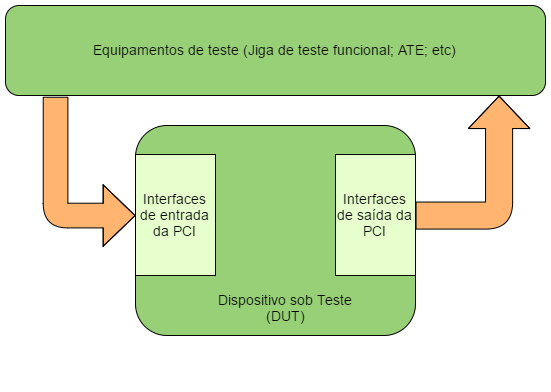
\includegraphics[width=0.8\linewidth]{fig/functionaltest}
            \caption{Diagrama de blocos de um esquema de teste funcional}
            \label{fig:funcblock}
\end{figure}

%geração de roteiros e estado da arte
A geração do roteiro de teste geralmente é manual e os esforços de pesquisa em teste funcional se concentram em métodos de automatização da geração de testes. O trabalho de \citet{thibeault2006} propõe uma investigação em otimização de roteiros e reuso de padrões de teste gerados diretamente por ferramentas de validação de projeto. 

Também existem trabalhos mais recentes de automatização de testes funcionais, como o de \citet{riefert2014effective}, que desenvolveu um método automatizado para testes funcionais em processadores utilizando métodos formais.


%Em \citep{thibeault2006} ve-se que que é importante considerar que, mesmo com suas vantagens, é crescentemente difícil justificar o uso de testes funcionais em velocidade nominal como abordagem principal. Sob esta perspectiva, parece que um teste funcional em velocidade nominal será mais e mais restrito à partes do DuT sem suporte à varredura periférica \citep{thibeault2006}. Todavia, a captura de defeitos relacionados à temporização não é o único aspecto positivo do teste funcional. Sua natureza não serial também pode ser explorada para propósitos de otimização de testes. Em [But100], foi proposto a criação de um pequeno conjunto de padrões de teste moderadamente rápidos, inseridos de inicio no programa de teste, de maneira a obter vantagem de sua inicial má capacidade de detecção de dispositivos enquanto mantem custos de desenvolvimento a um nível aceitável. Estas propostas foram baseadas no fato de qeu é mais difícil e caro criar e depurar padrões quando a frequência do  padrão funcional é perto da velocidade especificada do dispositivo.

\section{Padrões de projeto em LabVIEW}

Padrões de projeto são formas bem estabelecidas para resolver problemas comumente recorrentes. Não se trata de um código fonte ou \textit{framework}, mas de uma descrição de como se resolver um problema que pode ser aplicado em diversas situações. Padrões de projeto ganharam popularidade na ciência da computação após a obra de \citet{gamma1994design}. 

As vantagens de usá-los estão na facilidade dos desenvolvedores em reconhecê-los no código fonte, de dispensarem a necessidade de reinventar soluções para problemas recorrentes, como também na confiança de estar aplicando uma solução bem trabalhada para um tipo de problema.

No caso específico do LabVIEW, os padrões de projeto podem ser um modelo como um \textit{framework}, ou seja, uma base de códigos para o desenvolvimento da aplicação. Em \citet{blume2007labview} descrevem-se os principais padrões de projeto e \textit{frameworks} da linguagem: as máquinas de estado; os laços acionados por evento; o produtor-consumidor; o tratador de mensagem em fila; a máquina de estados em fila; e o Modelo de Atores.

\subsubsection{Máquinas de Estados Finitos}
As máquinas de estados finitos (figura \ref{fig:statemachine}) são amplamente conhecidas e, nelas, o comportamento dinâmico do programa depende de estados cujas transições dependem de uma lógica de estados. É fundamental a criação de uma tabela de estados para uma máquina de estados efetiva.

\begin{figure}
    \centering
        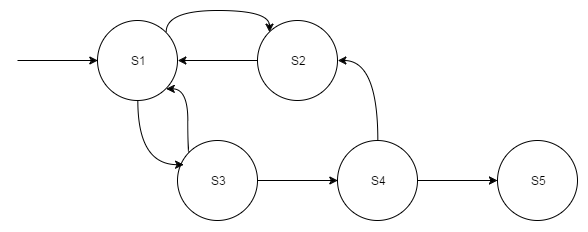
\includegraphics[width=0.8\linewidth]{fig/patt/statemachine}
            \caption{Um exemplo de máquina de estados finita}
            \label{fig:statemachine}
\end{figure}

\subsubsection{Laços Acionados por Eventos}
Nos laços acionados por eventos (figura \ref{fig:eventloop}), diferentemente do paradigma procedural, a execução do programa é decidida em tempo de execução: o programa permanece em estado de espera até a ocorrência de um evento e seu despacho para um tratador. Esta técnica poupa tempo de CPU e é uma boa alternativa ao uso de \textit{pooling}, além de poder ser aplicada em qualquer sistema de acionamento de processos escravos.

\begin{figure}[h]
    \centering
        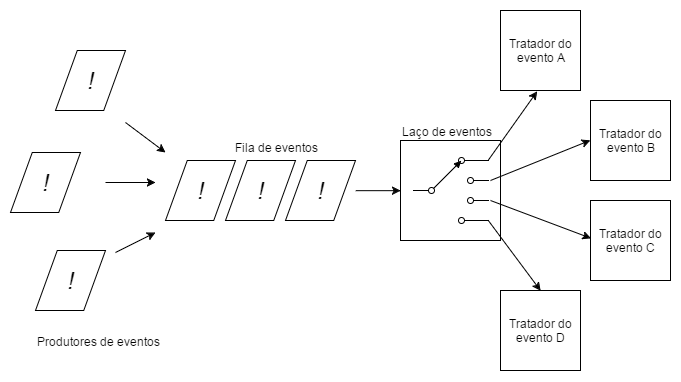
\includegraphics[width=1\linewidth]{fig/patt/eventloop}
            \caption{Laço acionado por eventos}
            \label{fig:eventloop}
\end{figure}

\subsubsection{O Produtor - Consumidor}
O produtor-consumidor (figura \ref{fig:prodcon}) é normalmente aplicado quando se precisa executar tarefas assíncronas e comunicar entre elas sem perda de desempenho, caso uma dependa da outra. Este padrão tem por característica a relação de mestre/escravo entre os laços e a independência no fluxo de dados entre eles. Uma tarefa produzindo dados ou comandos e uma ou mais tarefas consumindo o que a produtora gera. A comunicação entre as tarefas é realizada por filas, ou seja, os dados são enfileirados e desenfileirados em um \textit{buffer}, em esquema conhecido como \textit{first-in-first-out - FIFO}.

\begin{figure}
    \centering
        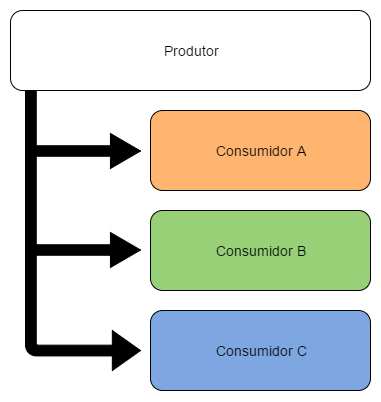
\includegraphics[width=0.5\linewidth]{fig/patt/produtorconsumidor}
            \caption{Diagrama do produtor-consumidor com 4 laços independentes comunicando por uma fila}
            \label{fig:prodcon}
\end{figure}

\begin{figure}
    \centering
        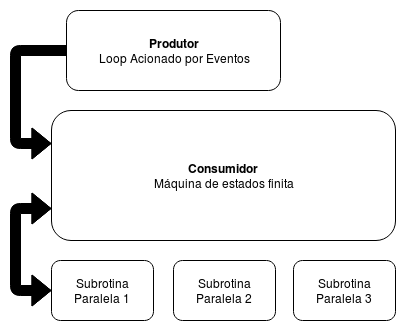
\includegraphics[width=0.7\linewidth]{fig/patt/tmf}
            \caption{Diagrama do tratador de mensagens em fila}
            \label{fig:tmf}
\end{figure}


\subsubsection{Tratador de mensagens em fila}
O tratador de mensagens em fila - TMF (figura \ref{fig:tmf}) ou, em inglês, \textit{Queue Message Handler} ou \textit{Queue-driven State Machine}, é uma extensão do produtor-consumidor, possibilitando que processos escravos possam atuar também como produtores e comunicar entre si. Normalmente apresenta-se como na figura \ref{fig:tmf}, com um laço mestre acionado por eventos criando tarefas, um processo principal e subprocessos auxiliares. O TMF não só é um padrão de projeto, mas também a arquitetura base de muitas aplicações de média a grande complexidade. É usado em aplicações que exijam interfaces de usuário responsivas, aplicações multitarefa e o desacoplamento de processos.


\subsection{Framework de Atores}
\label{actorframework}


%\subsubsection{A necessidade de um outro modelo de computação concorrente}

Na programação imperativa, assim como na maior parte dos paradigmas e linguagens de programação, as \textit{threads} são a solução tradicional para problemas de concorrência. Entretanto, programação concorrente baseada em \textit{threads}, \textit{locks} e estados compartilhados são ditas difíceis de fazer e propensas a erro \citep{Erb2012}. 

Em 1973, \citet{hewitt1973session} criou o modelo de atores como alternativa às \textit{threads} em problemas de computação concorrente e sistemas distribuídos. Sua premissa é a de que qualquer computação fisicamente possível pode ser diretamente implementada usando Atores \citep{hewitt2010actor}. 

 A abordagem no modelo de atores é totalmente diferente, já que retira inteiramente a noção de estado compartilhado. Ainda é possível que haja estados, entretanto, estes estão exclusivamente acoplados a uma única entidade, chamada Ator.

O modelo tem sido usado tanto como uma estrutura base para compreensão de problemas de concorrência, como também como base teórica para diversas implementações práticas de sistemas concorrentes. O crescimento de sistemas concorrentes massivos de computação em nuvem e processadores \textit{multi-cores} tem aumentado o interesse por este modelo. Exemplos de sistemas modelados pelo sistema de atores incluem: sistemas de email, Serviços Web e Objetos com \textit{locks}.

\subsubsection{Conceitos fundamentais do modelo}

Um ator é a unidade primitiva de computação. Ao receber uma mensagem, um ator pode concorrentemente \citep{hewitt2013computation}:

\begin{itemize}
    \item Criar um finito número finito de novos atores;
    \item Enviar finitas mensagens para outros atores;
    \item Designar como tratar a próxima mensagem que receber, alterando seu estado interno.
\end{itemize}

%Comunicação Assíncrona.
Para comunicação, o modelo de atores usa a troca de mensagens assíncronas, atribuindo a cada ator a sua caixa de mensagens (figura \ref{fig:actor}), local onde as mensagens são armazenadas enquanto o ator processa a mensagem anterior. Num sistema de atores, tudo o que um ator sabe do outro é o endereço de sua caixa de mensagens.

O ator sempre trabalha em resposta às mensagens que recebe, tratando-as sequencialmente, uma de cada vez \citep{Erb2012}. Isso significa que, para executar múltiplas mensagens de forma concorrente, será necessário que antes se crie um ator para cada uma delas. 

    \begin{figure}
        \centering
        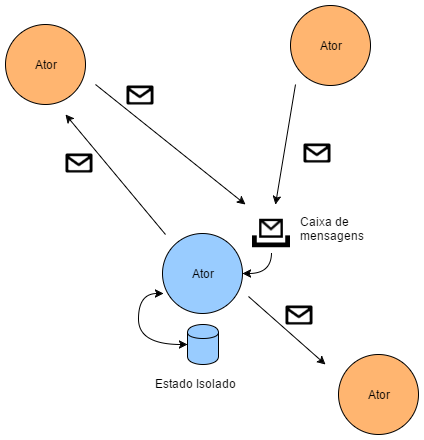
\includegraphics[width=0.9\linewidth]{fig/actor}
        \caption{Um exemplo de uma rede com alguns atores, com destaque para um ator, sua caixa de mensagens e seu estado interno. Adaptado de \citet{Erb2012}}
        \label{fig:actor}
    \end{figure}
 
O ponto central do modelo de atores, e o que o diferencia das \textit{threads}, é que não existe compartilhamento de memória ou estado, sendo completamente isolados uns dos outros. \citet{Erb2012} enfatiza que a implementação de estados privados é fundamental para um sistema no modelo de atores.

\subsubsection{Distribuição e Escalabilidade}

A natureza assíncrona e sem compartilhamento de estados do modelo de atores assemelha-se à comunicação em rede, o que permite a implementação de sistemas distribuídos. De fato, muitas das implementações do modelo de atores oferecem essa funcionalidade e possibilitam a fácil extensão do sistema para múltiplas máquinas em um sistema concorrente e distribuído \citep{hewitt2010actor, Erb2012}. 

Pela sua simplicidade e isolamento entre atores, o modelo permite o escalonamento de aplicações pelo instanciamento e replicação de atores e distribuição por outras máquinas.

\subsubsection{Robustez e tolerância a falhas em tempo de execução}

Sistemas concorrentes baseados em \textit{threads} dificilmente conseguem ter boas soluções de tolerância a faltas por causa do não-determinismo associado ao compartilhamento de estados e apreensão de recursos (\textit{locks}) \citep{Erb2012}. 

O modelo de atores normalmente adota uma política de \textit{deixar quebrar}. Isso porque a maneira isolada e de não compartilhar nada dos atores permite que um ator quebre sem influenciar os outros atores. Além do mais, pode-se usar atores em hierarquia para supervisionar possíveis falhas de atores \textit{filhos}, conforme visto em \citet{Erb2012}. Isso permite criar sistemas que se recuperem sozinhos, de forma que, se um ator do sistema quebrar, o sistema tem como detectar o problema e colocar o sistema em um estado consistente novamente. 

A política de deixar quebrar é enxuta, já que dispensa a necessidade de criar infinitos tratadores para muitos problemas, que talvez nunca ocorram, e a implementação de outras politicas de Programação Defensiva.

% Overly defensive programming however introduces unnecessary code for errors impossible to even happen, thus wasting runtime and maintenance costs. There is also the risk that the code traps or prevents too many exceptions, potentially resulting in unnoticed, incorrect results.https://en.wikipedia.org/wiki/Defensive_programming

\subsection{Implementação em LabVIEW}

O modelo de atores possui implementações em inúmeras linguagens, tanto no paradigma orientado a objetos, como também no paradigma funcional. Em LabVIEW, sua implementação foi realizada por meio de um \textit{framework}, ou seja, uma estrutura básica de programa na qual uma aplicação pode ser construída.

No texto de \citet{smithAF}, constata-se que esta implementação é mais restrita do que em outras linguagens. Primeiro que, no \textit{framework} de atores, a comunicação de um ator é limitada a mensagens para o ator que o criou, atores que ele criou ou para sí mesmo (ver figura \ref{fig:actormsg}). Essa hierarquia, por um lado, obriga a criar atores supervisórios, mas também restringe a comunicação entre a rede de atores.

A implementação dos atores não são estruturas leves e \textit{atômicas} como proposto por \citet{hewitt1973session}, mas objetos sobrecarregados por diversas camadas de sub-rotinas\footnote{Uma sub-rotina em LabVIEW é também referida como \textit{subVirtual Instrument} ou \textit{subVI}.}. Isto impede a construção e destruição irrestrita de atores. Todavia, o \textit{framework} ainda detém grande flexibilidade de arranjos de atores e hierarquias de programa.


\begin{figure}[h!]
    \centering
    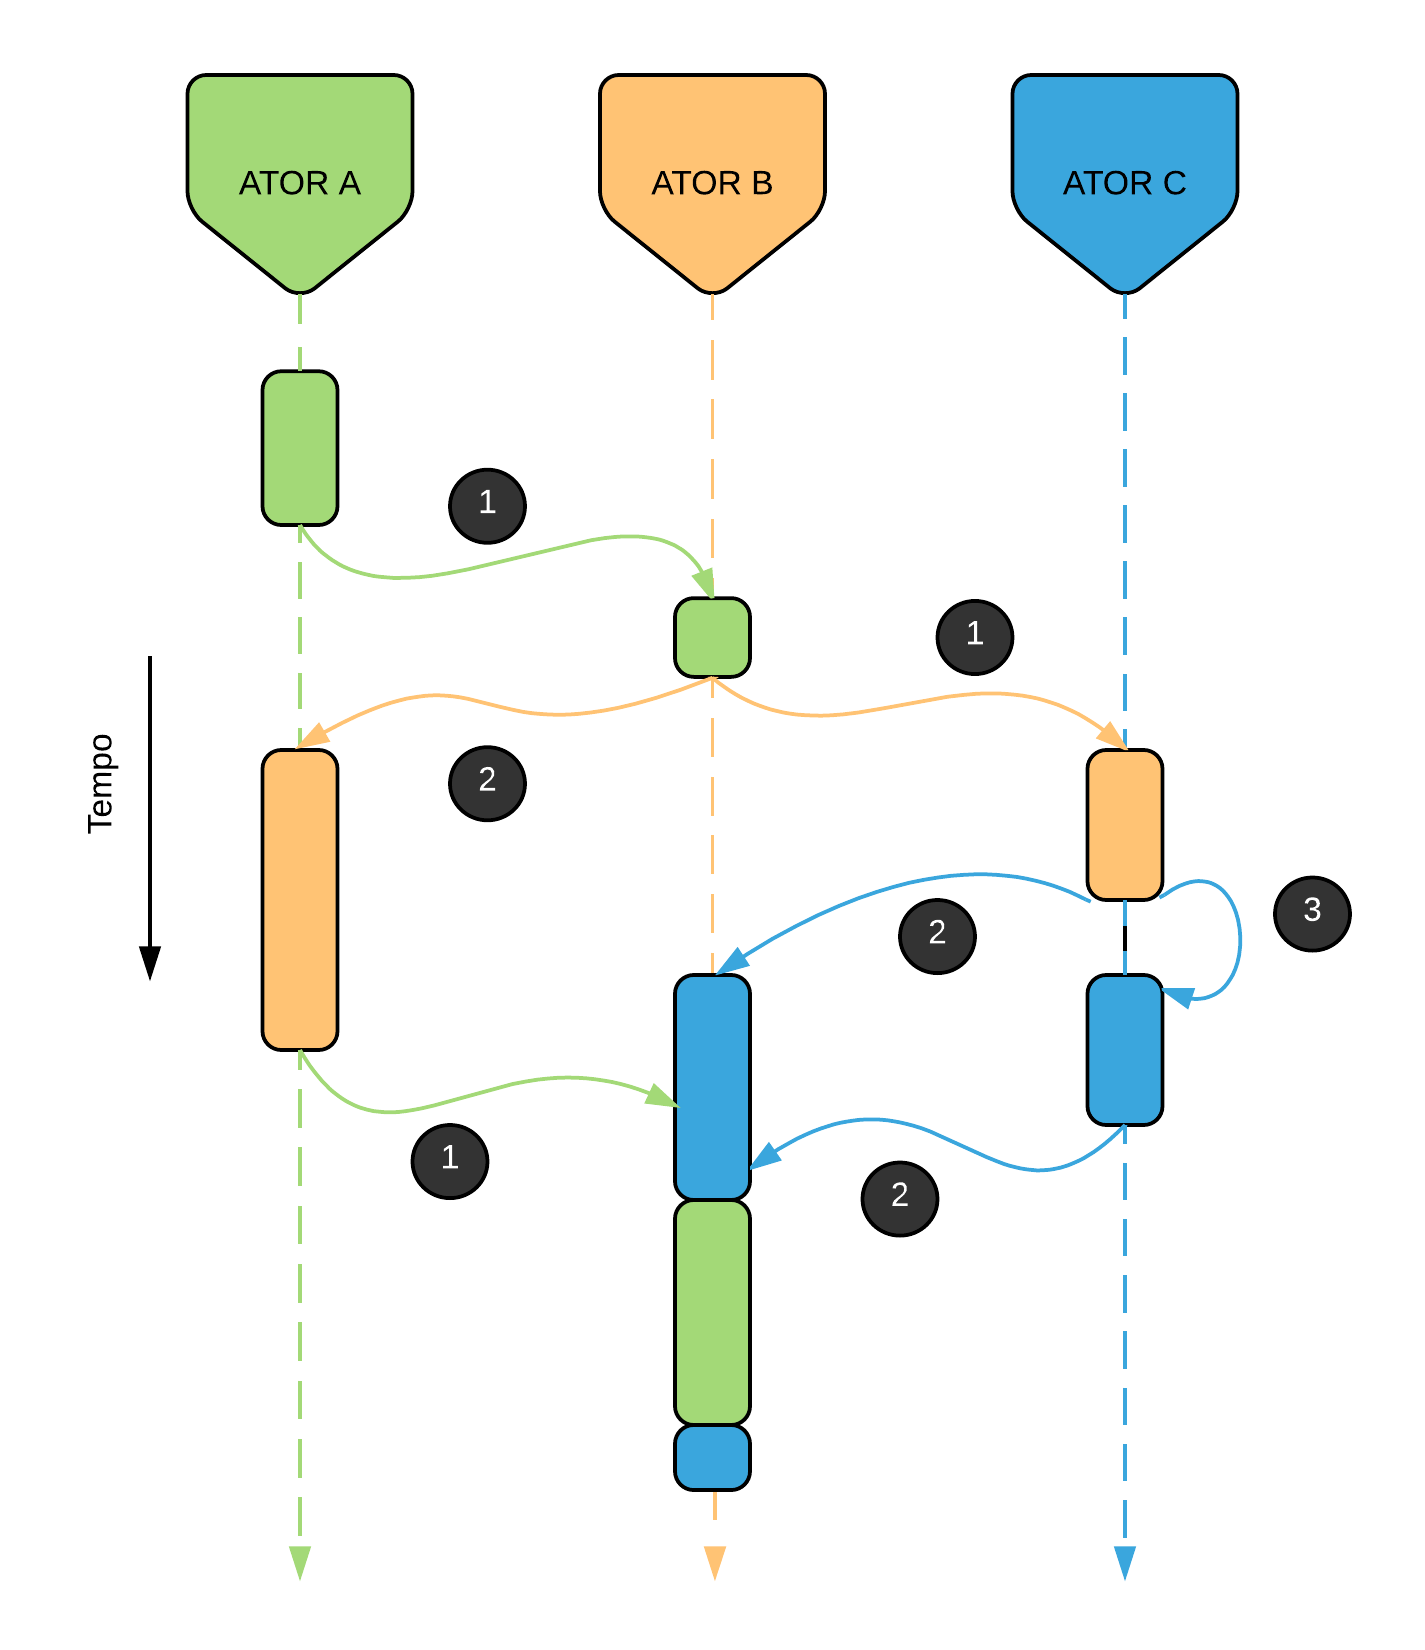
\includegraphics[width=0.9\linewidth]{fig/actormsg}
    \caption{Mensagens no \textit{framework} de atores em LabVIEW: (1) atores podem mandar mensagens para seus filhos; (2) atores podem mandar mensagem para os seus pais; (3) atores podem mandar mensagem para si mesmos}
    \label{fig:actormsg}
\end{figure}

Um ponto curioso do \textit{framework} é o suporte às mensagens síncronas entre atores \citep{smithAF}, funcionalidade que cria um compartilhamento de estado e rompe com a proposta do modelo.

% https://books.google.com.br/books?hl=en&lr=&id=s4AR6y1cp5EC&oi=fnd&pg=PA159&dq=actor+model&ots=x-POw6gaOc&sig=AhvfbolBXNsxexNgxGVpMoqShKs#v=onepage&q=actor%20model&f=false
% https://arxiv.org/ftp/arxiv/papers/1008/1008.1459.pdf
% http://berb.github.io/diploma-thesis/original/054_actors.html

\begin{comment}

O que eu quero falar na revisão?
Esta revisão bibliográfica pretende atingir dois objetivos: a revisão do estado da arte em teste de  placas eletrônicas, e também dos fundamentos do uso de programação concorrente, foco deste trabalho


Definir teste e diagnóstico.
Teste é o procedimento de checagem realizado para garantir a qualidade, desempenho, e confiabilidade de algo antes de ser colocado em uso
Diagnóstico é a identificação de uma causa raiz de um problema pela examinação de seus sintomas.
Metricas

O que eu quero falar na revisão?
Esta revisão bibliográfica pretende atingir dois objetivos: a revisão do estado da arte em placas eletrônicas, e também dos fundamentos do uso de programação concorrente, foco deste trabalho
\end{comment}
    %\chapter{Uma revisão sobre teste sistêmico}
%\addcontentsline{toc}{chapter}{Uma revisão do estado da arte em teste sistêmico, estrutural e funcional}

\section{Desafios no teste e validação de sistemas}

Conforme a literatura acadêmica \citep{jutman2014high} e também como prática da industria, o teste sistêmico tem de ser feito não somente após a manufatura, mas também para validação do sistema assim como no restante de seu ciclo de vida para manutenção e no diagnóstico dos retornos de campo. 

A complexidade destes sistemas requer - e ao mesmo tempo limita - a aplicação de uma abordagem de \textit{dividir para conquistar}. E é essencial realizar teste e diagnóstico de todos os componentes. Em caso  de encapsulamentos caros, a confiabilidade é um pouco maior, já que pra estes componentes existem políticas de \textit{Known Good Dies} (KGD)\footnote{Os circuitos são todos testados na própria fábrica, ainda nos waffers} e \textit{post-silicon validation} \citep{gilg1997known}. Mesmo assim isso somente não é suficiente já que suas interações com outros componentes do sistema também precisam ser validadas. Além disso, a integração e interação dos sistemas com o mundo real requerem o teste de propriedades não-funcionais como consumo de energia, desempenho térmico, e robustez sob diversas condições ambientais \citep{mitra2010post,ko2008distributed, jutman2014high}.

\section{Teste e diagnóstico no processo produtivo}

Dependendo da tecnologia utilizada, placas de circuito impresso podem ou não ser reparáveis. Independente disso, o dispositivo defeituoso precisa ser identificado e o diagnóstico é essencial tanto para o reparo quando para melhorias do processo produtivo \citep{ye2013board}. Se o reparo não é possível nas tecnologias avançadas, o diagnóstico ainda é necessário para compreender o problema e melhorar a produção. Pelas mesmas razões, \textit{SoCs} de sistemas defeituosos acabam também sujeitos a diagnósticos de falha \citep{tang2007analyzing, jutman2014high}.

\section{Diagnóstico na manutenção e retornos de campo}

Conforme \citet{jutman2014high}, a taxa de falha em campo pode ser interpretada como uma medida da dependência e da confiabilidade dos sistemas, e faz-se necessário que metas bem especificas das taxas de retorno sejam mantidas ou melhoradas. Isso também é importante no contexto de Controle de Qualidade e também para a alcançar certificações ISO.

O diagnóstico de sistemas eletrônicos é fundamental, e, em setores de aplicação como automotivo ou aeroespacial, a causa raiz de toda e qualquer falha sistêmica precisa ser esclarecida \citep{abelein2014non}. Em casos como esses, dois desafios precisam ser superados: Primeiramente, muitas falhas somente são observáveis sob condições específicas de operação, podendo desaparecer após a desmontagem do sistema (Jutman et al.,2014). 

Estes casos de \textit{Falha Não Encontrada} (ou em inglês, \textit{"No Failure Found"} ou NFF) acabam tornando-se caros e também introduzem riscos para outros produtos \citep{conroy2005practical}. Em segundo lugar, o OEM - \textit{Original Equipment Manufacturer}, como por exemplo um fabricante de veículos, depende de uma grande cadeia de fornecedores, e a identificação de falhas requer a colaboração de muitos parceiros (Figura 1-a). Segundo \citet{jutman2014high}, se as PCIs e circuitos integrados oferecerem uma boa capacidade de auto-diagnostico para o OEM, isso ajudaria a encurtar o processo de diagnóstico (Figura 1-b), além de poder ser usado sob condições típicas de operação para reduzir os NFF antes da desmontagem do sistema. Os dados coletados beneficiariam não só o OEM como também todos os membros da cadeia produtiva \citep{cook2014diagnosis}.
    \begin{figure}
        \centering
        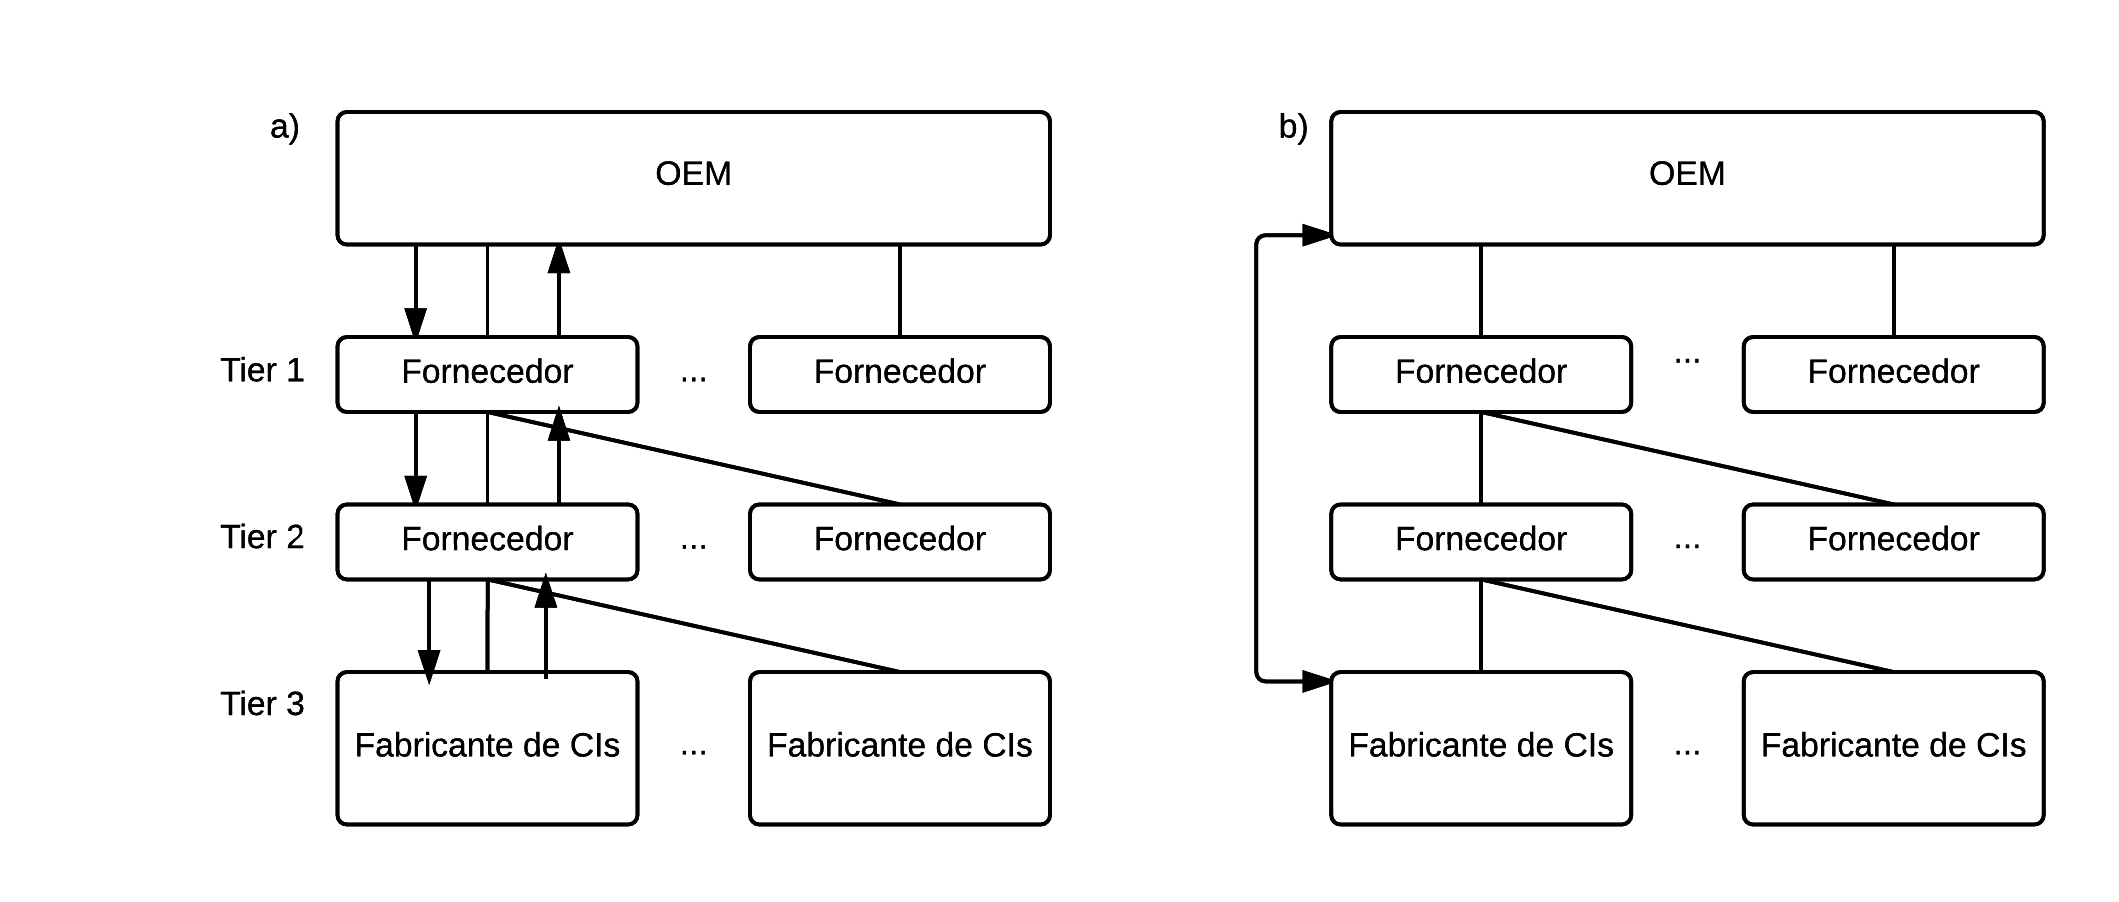
\includegraphics[width=.8\linewidth]{oem}
        \label{fig:supplychain}
        \caption{Diagnóstico do sistema no decorrer da cadeia de fornecedores. Adaptado de Jutman (2014)}
    \end{figure}
Dados de teste também podem ser coletados em campo \textit{on-line} e \textit{off-line} ou em concorrência ou não-concorrência. As respostas dos testes registradas em campo podem ajudar a diagnosticar os retornos de campo. Além do mais este tipo de teste é necessário para a checagem de funcionalidade de sistemas críticos (safety-critical systems).

O próximo capitulo descreve as práticas comuns, atuais desafios e técnicas avançadas em testes à nível de placa. E os capítulos seguintes especificam sobre testes estruturais e testes funcionais.

    %\chapter{Teste de PCI: práticas comuns, desafios atuais e técnicas avançadas}
%\addcontentsline{toc}{chapter}{Teste de PCI: práticas comuns, desafios atuais e técnicas avançadas}

O teste de fim de linha de manufatura realizado nas PCIM é um dos procedimentos de teste finais antes de embalar e entregar o produto. Tipicamente, cada montagem de placa produzida tem que passar em variadas fases de teste antes de ser qualificada para expedição. O montante destas fases de teste pode ser numerosas para um produto eletrônico complexo e depende também da qualidade, e confiabilidade dos seus requerimentos de projeto (Jutman et al., 2014). 

Cada classe de teste é especializada para uma gama limitada de defeitos, e é custoso, senão impossível, forçar a cobertura de defeitos fora daqueles que tal classe tenta resolver. Dessa maneira, a solução normalmente adotada é combinar diversas técnicas de teste (Jutman et al., 2014). Dessa maneira, uma estratégia de teste eficiente para um produto complexo tipicamente requer ao menos uma técnica para cada categoria exibida na Tabela \ref{tab:testcategories}. Considera-se também que combinação de técnicas de teste é também ditada por sua viabilidade econômica \citep{davis1994economics}.

\newpage

\begin{table}[]
\centering
\caption{Principais categorias em teste de Placas de Circuito Impresso montadas - PCIMs. Traduzido de Jutman (2014)}
\label{tab:testcategories}
\begin{tabular}{ll}
\hline
\rowcolor[HTML]{EFEFEF} 
\multicolumn{1}{|l}{\cellcolor[HTML]{EFEFEF}{\color[HTML]{000000} }}                                   & \multicolumn{1}{l|}{\cellcolor[HTML]{EFEFEF}{\color[HTML]{000000} \textit{Pré-reflow: SPI\footnotemark, AOI\footnotemark  }}}                 \\ \cline{2-2} 
\rowcolor[HTML]{EFEFEF} 
\multicolumn{1}{|l}{\multirow{}{}{\cellcolor[HTML]{EFEFEF}{\color[HTML]{000000} \textbf{Inspeção}}}}         & \multicolumn{1}{l|}{\cellcolor[HTML]{EFEFEF}{\color[HTML]{000000} \textit{Pós-reflow: Inspeção Visual, AXI\footnotemark, AOI}}}                 \\
\rowcolor[HTML]{C0C0C0} 
\multicolumn{1}{|l}{\cellcolor[HTML]{C0C0C0}{\color[HTML]{000000} \textbf{Teste Elétrico}}}                     &  \multicolumn{1}{l|}{\cellcolor[HTML]{C0C0C0}{\color[HTML]{000000} \textit{ICT, MDA, FPT\footnotemark}}}           \\
\rowcolor[HTML]{9B9B9B} 
\multicolumn{1}{|l}{\cellcolor[HTML]{9B9B9B}{\color[HTML]{000000} \textbf{Teste de Sondagem}}}                  & \multicolumn{1}{l|}{\cellcolor[HTML]{9B9B9B}{\color[HTML]{000000} \textit{Boundary Scan}}}             \\
\rowcolor[HTML]{656565} 
\multicolumn{1}{|l}{\cellcolor[HTML]{656565}{\color[HTML]{FFFFFF} Teste em alta velocidade}} & \multicolumn{1}{l|}{\cellcolor[HTML]{656565}{\color[HTML]{FFFFFF} Teste centralizado por..}}            \\
\rowcolor[HTML]{343434} 
\multicolumn{1}{|l}{\cellcolor[HTML]{343434}{\color[HTML]{FFFFFF} Instrumentação Embarcada}}           & \multicolumn{1}{l|}{\cellcolor[HTML]{343434}{\color[HTML]{FFFFFF} Instrumentação BIST (Hardware Fixo)}} \\ \hline
\rowcolor[HTML]{000000} 
{\color[HTML]{FFFFFF} Teste Funcional}                                                                 & {\color[HTML]{FFFFFF} Testes de interfaces e etc.}                                                                                 \\ \hline
\end{tabular}
\end{table}
%bug
\footnotetext[1]{Inspeção de pasta de solda ou em inglês: \textit{Solder Paste Inspection -- SPI}}
\footnotetext[2]{Inspeção Ótica Automatizada ou em inglês \textit{Automated Optical Inspection -- AOI}}
\footnotetext[3]{Inspeção Radiográfica Automatizada ou em inglês \textit{Automated X-Ray Inspection -- AXI}}
\footnotetext[4]{Respectivamente: Teste In-Circuit, Manufacturing Defect
Analysis, Flying Probe Test}

\section{Sondagem periférica para a inspeção de PCIM}

Técnicas de inspeção ajudam a checar a integridade geral da placa montada como presença de componentes, polaridade, qualidade de solda, pinos levantados, etc. E conforme Jutman (2014), testes de sondagem periférica - como o JTAG / \textit{Boundary Scan} -  são hoje o padrão da industria de teste em nível de placa pois promovem uma tecnologia de teste barata e eficiente em termos de cobertura e capacidade de resolução de problemas \nocite{parker2012boundary}. O iNEMI fez uma pesquisa em 2009 \citep{geiger2009boundary} que corroboa isso: aproximadamente 80\% dos engenheiros de teste consideram de importância alta ou moderada a inserção de testes de sondagem periférica como uma de suas táticas de verificação de seus produtos, até mesmo pela redução no custo de geral desenvolvimento que essa categoria de teste promove (Jutman et al., 2014). 

Na tabela \ref{tab:boundaryscanfamily}., podemos ver a todas as variações de Sondagem periférica e suas respectivas finalidades. O padrão IEEE 1149.1 \citep{ieee11491old} é o antecessor de toda a família e prove o conceito básico da arquitetura e os princípios de acesso de teste (Jutman et al., 2014). A última versão do IEEE 1149.1 foi publicada em 2013 \citep{ieee11491yr2013} com grandes atualizações incorporadas, incluindo padronizações de meios de controle de instrumentação embarcada e condicionamento de sinais a nível de pinagem.

\begin{table}[]
\centering
\tiny
\caption{Padrões IEEE de acesso ao teste baseado em sondagem. Adaptado de Jutman (2014)}
\label{tab:boundaryscanfamily}
\begin{tabular}{p{50}p{50}p{50}p{50}}
\hline
\rowcolor[HTML]{C0C0C0} 
\multicolumn{1}{|p{50pt}|}{\cellcolor[HTML]{C0C0C0}\textbf{Foco principal de aplicação}} & \multicolumn{1}{p{50pt}|}{\cellcolor[HTML]{C0C0C0}\textbf{Propósito Principal}} & \multicolumn{1}{p{50pt}|}{\cellcolor[HTML]{C0C0C0}\textbf{Base da Tecnologia}}    & \multicolumn{1}{p{50pt}|}{\cellcolor[HTML]{C0C0C0}\textbf{Classes de falta a serem cobertas}}     \\
\rowcolor[HTML]{656565} 
\multicolumn{4}{|l|}{\cellcolor[HTML]{656565}{\color[HTML]{FFFFFF} \textbf{IEEE 1149.1 - Boundary Scan \citep{ieee11491old, ieee11491yr2013}}}}                                                                                        \\
\multicolumn{1}{|p{50pt}|}{Teste de Manufatura de PCI}                                        & \multicolumn{1}{p{50pt}|}{Melhorias de acesso aos testes}                               & \multicolumn{1}{p{50pt}|}{Registradores de sondagem on-chip}                            & \multicolumn{1}{p{50pt}|}{Faltas em pinos e integridade de circuto}                                 \\
\rowcolor[HTML]{656565} 
\multicolumn{4}{|l|}{\cellcolor[HTML]{656565}{\color[HTML]{FFFFFF} \textbf{IEEE 1149.4 - Barramento para testes de sinais mistos \citep{ieee11494} .}}}\\

\multicolumn{1}{|p{50pt}|}{Medição de sinais analógicos} &
\multicolumn{1}{p{50pt}|}{Melhorias de acesso aos testes} & 
\multicolumn{1}{p{50pt}|}{Chaves \textit{on-chip}} &
\multicolumn{1}{p{50pt}|}{Valores paramétricos}\\

\rowcolor[HTML]{656565} 
\multicolumn{4}{|l|}{\cellcolor[HTML]{656565}{\color[HTML]{EFEFEF} \textbf{IEEE 1149.6 - Teste BST de Redes Digitais Avançadas \citep{ieee11496}}}}\\

\multicolumn{1}{|p{50pt}|}{Teste de redes LVDS de alta velocidade} &
\multicolumn{1}{p{50pt}|}{Teste de malhas acopladas em corrente alternada} & 
\multicolumn{1}{p{50pt}|}{Geradores de pulsos \textit{on-chip}} &
\multicolumn{1}{p{50pt}|}{integridade de malha}\\

%\rowcolor[HTML]{656565} 
\multicolumn{4}{|l|}{\cellcolor[HTML]{656565}{\color[HTML]{EFEFEF} \textbf{IEEE 1149.7 - Pinos reduzidos e TAP aprimorado \citep{ieee11497}}}}\\

\multicolumn{1}{|p{50pt}|}{Teste de placa e debug de software} &
\multicolumn{1}{p{50pt}|}{Acesso à teste flexivel e em alta velocidade por dois pinos} & 
\multicolumn{1}{p{50pt}|}{SERDES, endereçamento} &
\multicolumn{1}{p{50pt}|}{Contempla todos acima}\\

%\rowcolor[HTML]{656565} 
\multicolumn{4}{|l|}{\cellcolor[HTML]{656565}{\color[HTML]{EFEFEF} \textbf{IEEE 1149.8.1 - Alternância de pinos e sensoriamento sem contato\citep{ieee114981}}}}\\

\multicolumn{1}{|p{50pt}|}{Teste de interconexão de PCIM} &
\multicolumn{1}{p{50pt}|}{Ligações para componentes passivos} & 
\multicolumn{1}{p{50pt}|}{chapas de sensoriamento capacitivo} &
\multicolumn{1}{p{50pt}|}{Circuitos abertos: AC e DC }\\

\multicolumn{4}{|l|}{\cellcolor[HTML]{656565}{\color[HTML]{EFEFEF} \textbf{IEEE P1149.10- TAP de alta velocidade \citep{ieeep1149102016} }}}\\

\multicolumn{1}{|p{50pt}|}{O mesmo que todos acima} &
\multicolumn{1}{p{50pt}|}{Permutação de dados de teste em alta velocidade} & 
\multicolumn{1}{p{50pt}|}{Reuso de pinos I/O de alta velocidade} &
\multicolumn{1}{p{50pt}|}{O mesmo que todos acima}\\

\multicolumn{4}{|l|}{\cellcolor[HTML]{656565}{\color[HTML]{EFEFEF} \textbf{IEEE 1500 - Teste de núcleo embarcado \citep{ieee1500}}}}\\

\multicolumn{1}{|p{50pt}|}{Teste à nível de SoC e IP} &
\multicolumn{1}{p{50pt}|}{Acesso ao teste de \textit{IP cores} em um SoC} & 
\multicolumn{1}{p{50pt}|}{invólucros de núcleos} &
\multicolumn{1}{p{50pt}|}{Faltas no domínio digital dentro de um CI}\\

\multicolumn{4}{|l|}{\cellcolor[HTML]{656565}{\color[HTML]{EFEFEF} \textbf{IEEE 1687 - Acesso por Instrumentação Embarcada \citep{ieee1687}}}}\\

\multicolumn{1}{|p{50pt}|}{Teste de CI, debug, diagnóstico} &
\multicolumn{1}{p{50pt}|}{Padrão de acesso por instrumento} & 
\multicolumn{1}{p{50pt}|}{Cadeias de sonda reconfiguráveis} &
\multicolumn{1}{p{50pt}|}{Específicas do instrumento}\\

\multicolumn{4}{|l|}{\cellcolor[HTML]{656565}{\color[HTML]{EFEFEF} \textbf{IEEE P1838 - Acesso a teste para CIs 3D \citep{ieeep18382016}}}}\\

\multicolumn{1}{|p{50pt}|}{Teste de integração 3DSIC} &
\multicolumn{1}{p{50pt}|}{Acesso à teste através das vias TSV} & 
\multicolumn{1}{p{50pt}|}{O mesmo que os 150pt0, 1149.1, 1687} &
\multicolumn{1}{p{50pt}|}{Integridade das vias TSV}\\
\hline


\end{tabular}
\end{table}

\section{Técnicas avançadas e emergentes em teste de PCIMs}\label{advPCBA}

A maior limitação da sondagem periférica clássica é a incapacidade de aplicar padrões de teste na velocidade nominal de operação, dessa forma limitando o espectro de faltas cobertas em faltas estáticas, no domínio de corrente contínua (Jutman et al., 2014). Enquanto a alternativa clássica da industria sempre foi o uso de testes funcionais cuidadosamente elaborados, as companhias de ponta estão adotando técnicas emergentes de teste em alta-velocidade ou em velocidade real de execução baseadas em (re)configuração automática ou programação de dispositivos programáveis \textit{on-board} como FPGAs (referidos como teste centralizado \citep{aleksejev2013fpga} ou controlado \citep{jutman2014high} por FPGAs) e processadores (referidos como testes centralizados \citep{ehrenberg2009combining} ou controlados \citep{tsertov2011soc} por processador). Estas técnicas dependem da infraestrutura JTAG para o controle de fluxo de teste ao passo que convertem o FPGA/CPU \textit{on-board} em testadores embarcados (Jutman et al., 2014). Além da capacidade de cobrir faltas relacionadas à temporização (\textit{delays, crosstalk}, faltas no domínio AC), estas técnicas proporcionam um baixo grau de acesso para testes devido ao fato que os FPGA/CPUs são tipicamente, por predefinição, componentes da espinha dorsal de complexos dispositivos digitais e de sinais mistos \citep{6401571}. Ao término da rotina de testes, a configuração de teste é apagada e a placa é configurada para seu modo funcional. Dessa maneira, nenhum outro custo excessivo em \textit{Design for Test} adicional é necessário. Hoje, somente algumas companhias líder no setor JTAG oferecem ferramentas completamente automatizadas que suportam esta classe de testes como parte de seu pacote de programas.\par
Outra grande classe tecnológica emergente em testes à nivel de placa, cuja adesão atual ainda engatinha, é a \textit{instrumentação embarcada} \citep{embeddedinstrument}. Segundo Jutman (2014), no contexto de testes em PCIM, duas sub-classes marjoritárias de instrumentação embarcada podem ser citadas: 
\begin{itemize}
\item circuitos embarcados permanentemente fixos principalmente em ASICs;
\item instrumentos multi-propósito sintetizados em FPGA;
\end{itemize}
Exemplos típicos do primeiro são BIST de memória ou PRPGs (\textit{pseudo-random pattern generation} e contadores para Teste de \textit{Bit-Error Rate} (em inglês, BERT) de um canal de comunicação. A falta de padronização e práticas comuns limitam a ampla adoção e reuso de tais instrumentos embarcados fixos à nível de placa, ainda que várias aplicações à nivel de circuito integrado de várias soluções BIST estejam florescendo. Diferentemente, a instrumentação embarcada sintetizada em sistemas centralizados em FPGAs é muito promissora para testes \citep{6401571}.\par
Por ser o componente central de uma placa, e por possibilitar a completa reconfiguração e reuso, o FPGA torna-se um ótimo testador embarcado. Alguns poucos sistemas de teste JTAG de ponta proporcionam plataformas de instrumentação embarcada sintetizável para as seguintes aplicações:
\begin{itemize}
\item Teste de memória e BIST;
\item Teste de \textit{bit-error rate} (BERT) em canais de comunicação (conexões \textit{gigabit};
\item Teste de barramentos comuns (LAN, SATA, PCIe, USB, CAN, LIN, I2C, SPI, etc.) e UART;
\item Teste sistêmico e programação de memórias não-voláteis (dispositivos flash);
\item Instrumentos definidos por usuário.
\end{itemize}

A instrumentação embarcada abre potencial sem precedentes para o \textit{acesso ao diagnóstico}, monitoramento, e testes em alta velocidade. Estudos mostram que a expectativa industrial para com os benefícios da adoção da instrumentação embarcada é atualmente muito alta \citep{frostsullivan2010}. Pesquisas industriais em andamento nesta área são muito ativas com dois focos principais: a) automação \citep{aleksejev2013fpga}; b) melhorias na cobertura de falhas. O novo padrão IEEE 1687 - \textit{IJTAG} abre a porta na direção da integração perfeita de ferramentas, algoritmos, instrumentos, cores IP, e padrões de teste \citep{crouch2007ijtag}.

\section{Modelos de faltas e métricas de testabilidade à nivel PCIM}
Existem diversos pontos de vista na categorização, enumeração, e estimativa de cobertura de defeitos à nivel de placa, como pode ser visto na tabela \ref{metricas}.

\begin{table}[]
\tiny
\centering
\caption{Diferentes abordagens para as métricas de cobertura de teste. Fonte: Jutman et al. \citep{jutman2014high}}
\label{metricas}
\begin{tabular}{|m{50}|m{50}|m{50}|m{40}|}
\hline
\rowcolor[HTML]{9B9B9B} 
{\color[HTML]{000000} \textbf{Abordagem para a modelagem de falhas}} & {\color[HTML]{000000}\textbf{ Nível de abstração}}                      & {\color[HTML]{000000}\textbf{ Exemplos de defeitos}} & {\color[HTML]{000000}\textbf{ Métrica de cobertura de teste}}\\ \hline
{\color[HTML]{000000} Focando defeitos em materiais e feitos causados pelo processo de montagem}                             & \multicolumn{1}{m{50pt}|}{\color[HTML]{000000} Faltas estruturais em nível físico}                                                             & \multicolumn{1}{m{50pt}|}{\color[HTML]{000000} Solda ruim, terminais levantados ou tortos, componente defeituoso, desalinhamentos, efeito lápide, etc.} & \multicolumn{1}{m{40pt}|}{\color[HTML]{000000} PPVS, MPS, PCOLA / SOQ}\\ \hline
\multicolumn{1}{|m{50pt}|}{\color[HTML]{000000} Focando defeitos a nível de pino e malhas de circuito}                                                 & \multicolumn{1}{m{50pt}|}{{\color[HTML]{000000} Falhas estruturais e comportamentais a nível lógico}}                                            & \multicolumn{1}{m{50pt}|}{{\color[HTML]{000000} Circuitos abertos, ou em curto, defeito no driver (buffer, pino).}}                                       & \multicolumn{1}{m{40pt}|}{{\color[HTML]{000000} aaaaaaaaa}}  \\ \hline
\multicolumn{1}{|m{50pt}|}{{\color[HTML]{000000} Problemas funcionais causados por defeitos}}                                                            & \multicolumn{1}{m{50pt}|}{{\color[HTML]{000000} Defeitos a nível sistêmico (comportamental)}}                                                    & \multicolumn{1}{m{50pt}|}{{\color[HTML]{000000} Falha de boot, operação instável,}}                                                                       & \multicolumn{1}{m{40pt}|}{{\color[HTML]{000000} Métricas de cobertura de teste baseadas em modelo funcional}}                \\ \hline
\multicolumn{1}{|m{50pt}|}{{\color[HTML]{000000} Falhas relacionadas à performance principalmente em linhas de  interconexão , barramentos, interfaces, links de comunicação}} & \multicolumn{1}{m{50pt}|}{{\color[HTML]{000000} Principalmente abordagens estatísticas (taxas de erro); apesar de necessárias, ainda faltam abordagens estruturais.}} & \multicolumn{1}{m{50pt}|}{{\color[HTML]{000000} Falhas de alta taxa de erros (desempenho lento), crosstalk, jitter, delay;}}                                                   & \multicolumn{1}{m{40pt}|}{{\color[HTML]{000000} bit error rate em links de comunicação, mas não existe uma métrica abrangente na industria para uma métrica de cobertura de falhas estruturais}}\\ \hline
\end{tabular}
\end{table}

Ao passo que a modelagem de faltas estáticas\footnote{primeiras duas colunas da tabela \ref{metricas}.} (corrente contínua) tornou-se o padrão da indústria com pequenas atualizações que acompanhavam os progressos tecnológicos em montagem e integração como também os avanços tecnológicos de teste, o domínio AC\footnote{faltas relacionadas às altas velocidades, últimas duas linhas da tabela \ref{metricas}} representa hoje o maior desafio em termos de pesquisa e normatização (Jutman et al., 2014). Desconsiderando as medições de \textit{Bit Error Rate} (que retrata mais a qualidade do canal, i.e. relação sinal-ruído (SNR), do que a presença de um defeito estrutural especificamente), não há nenhuma métrica de larga abrangência industrial usada a nível de placa para medir qualidade de testes em alta velocidade ou velocidade nominal - como, por exemplo, os executados por instrumentação embarcada.

Os papéis dos testes estrutural e funcional podem ser resumidos pela figura \ref{fig:cobertura}:  Ambos se complementam. Os testes estruturais oferecem profundidade de teste em nível de pinos, e facilidade de automatização dos roteiros. Já o teste funcional abre portas para testes em tempo de execução, e a detecção de problemas que verificações estáticas não detectariam.

\begin{figure}[ht]
    \centering
    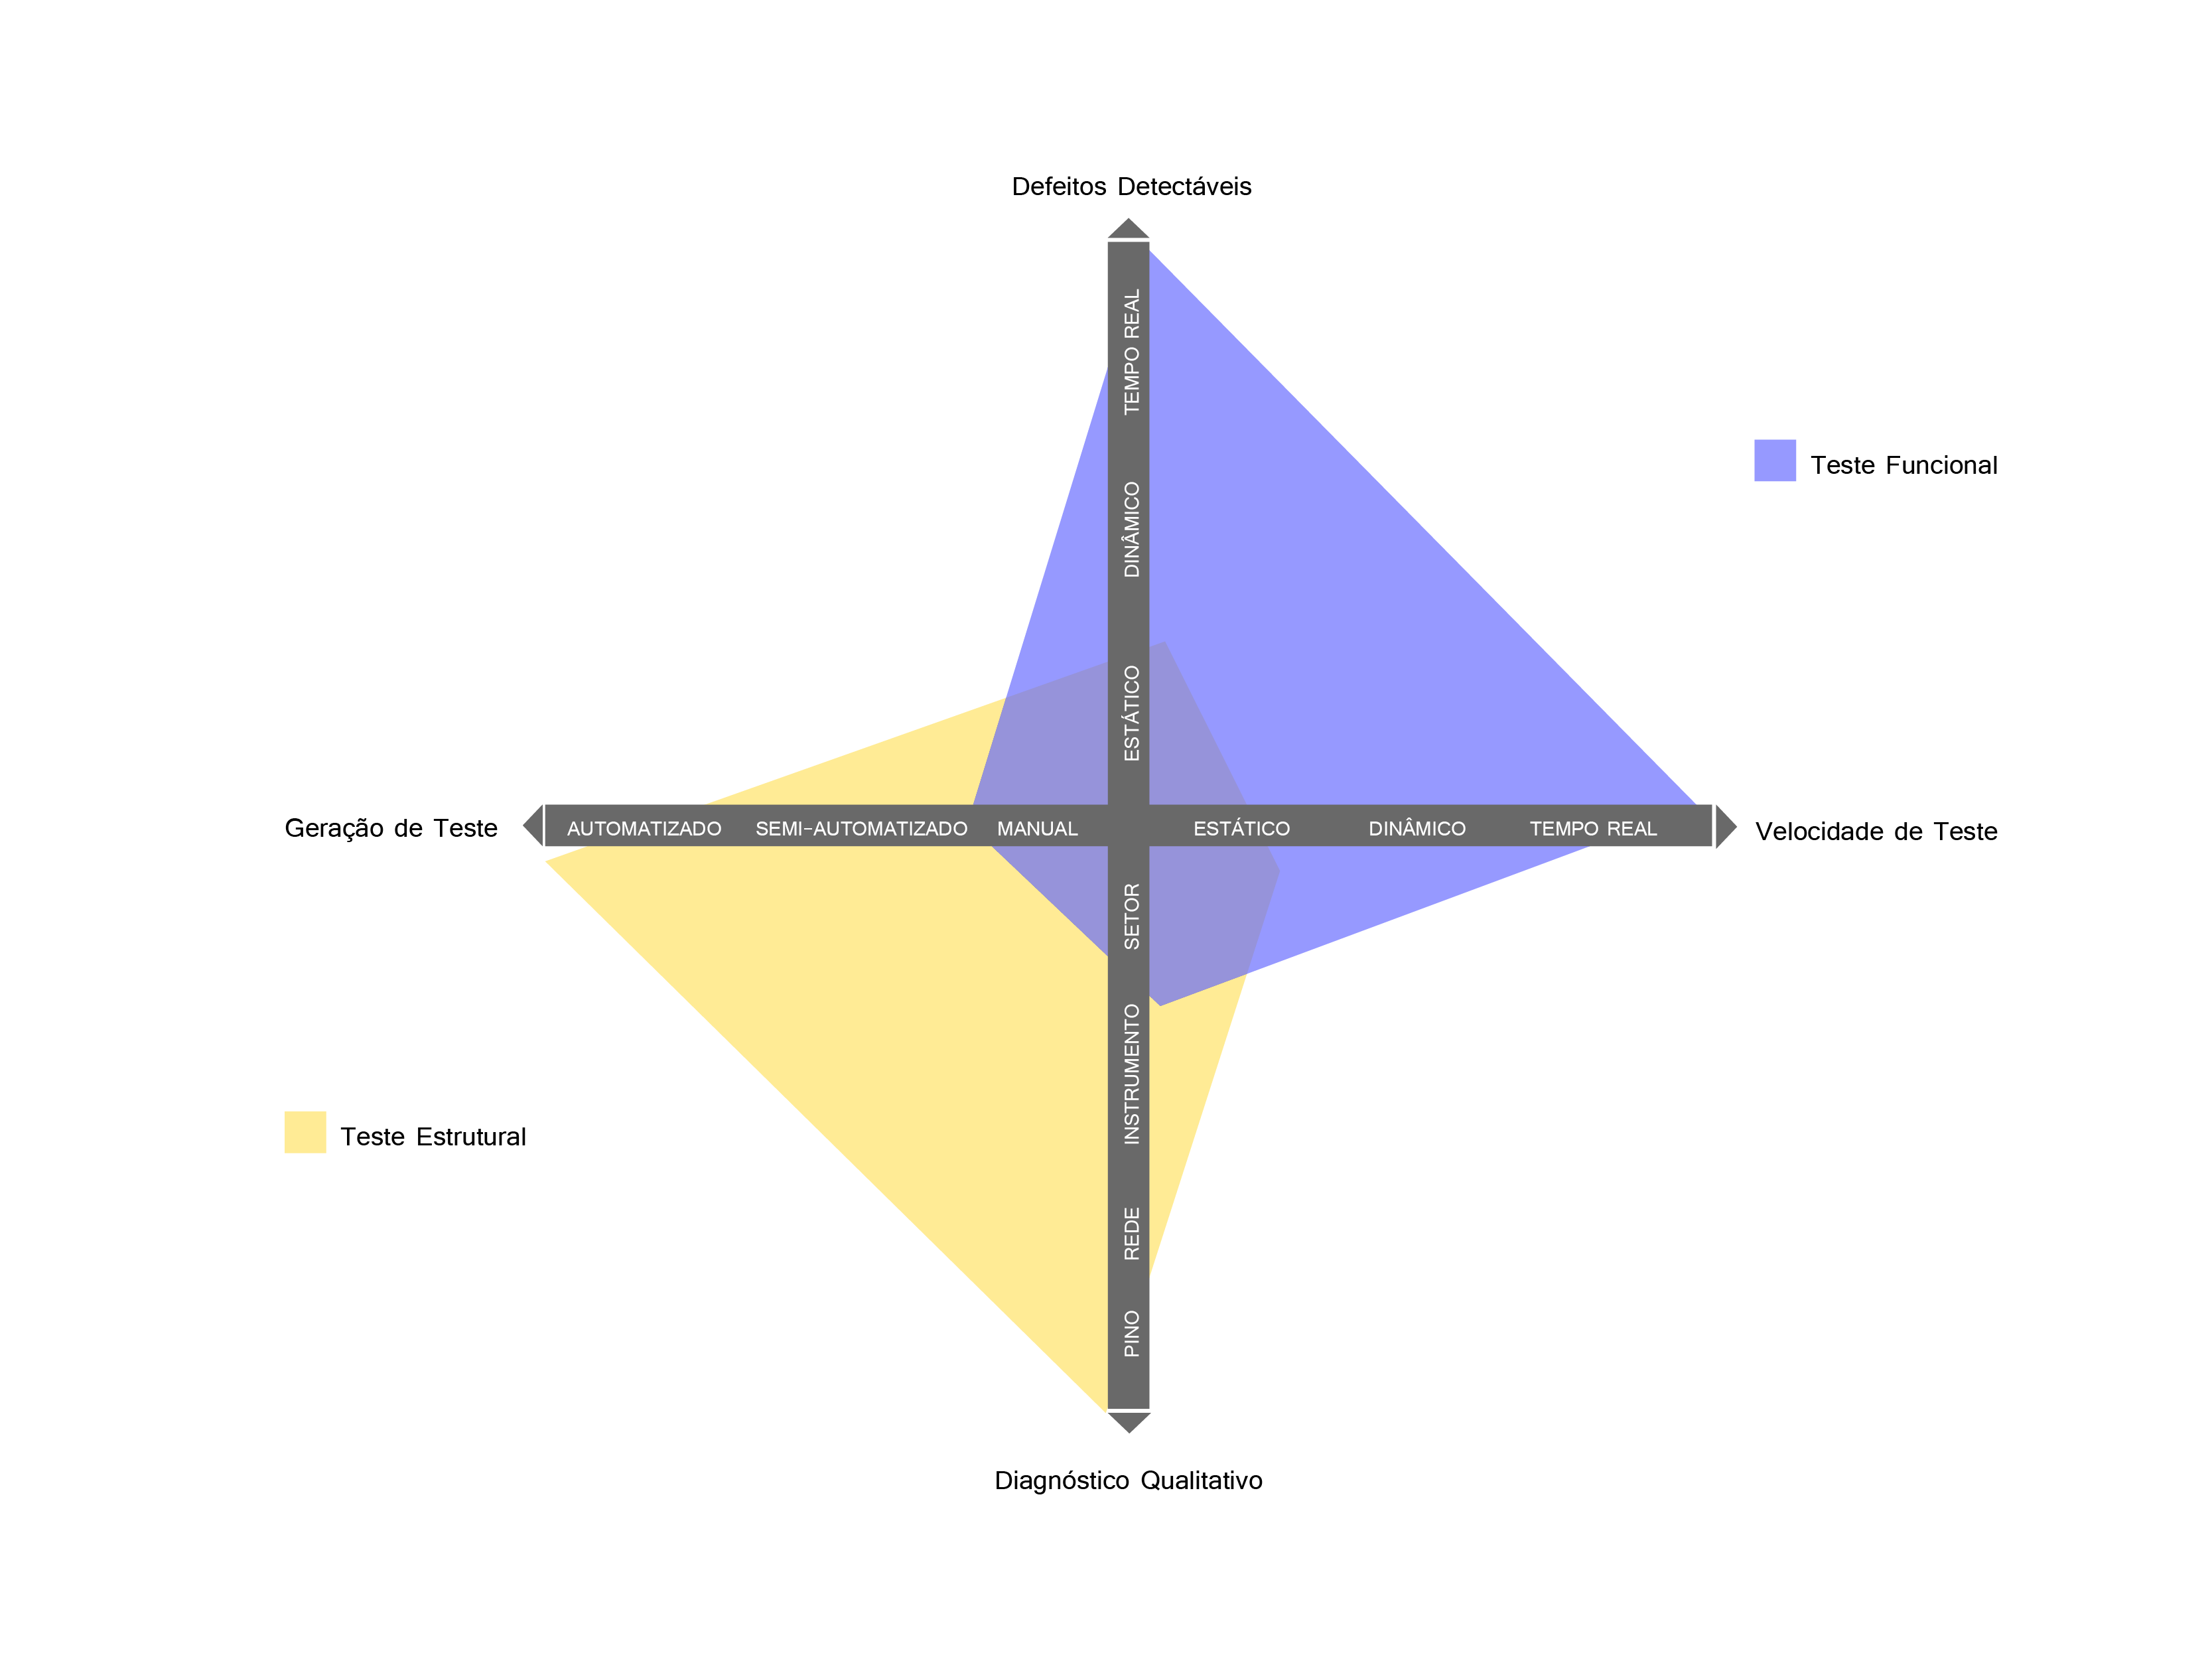
\includegraphics[width=1.2\linewidth]{coberturateste.png}
    \caption{A complementariedade dos testes estruturais e funcionais para a cobertura de teste de um dispositivo}
    \label{fig:cobertura}
\end{figure}

Segundo Jutman (2014), a própria falta de tecnologia dos aparelhos de medição e teste, resulta na impossibilidade de realizar verificações em velocidade nominal, o que impede uma cobertura de teste plena. Por sua vez, essas falhas na cobertura de teste -- que é algo dificilmente estimável -- contribui para problemas sérios de \textit{No-Failure Found (NFF)}, que são custosos para qualquer industria. Dessa forma, a pesquisa por melhores métricas de cobertura de teste, assim como na caracterização de defeitos, tornaram-se tópicos de pesquisa muito importantes.



%@article{embeddedinstrument
%How to test high-speed memory with non-intrusive embedded instruments. ASSE
    %\chapter*{Métodos Estruturais para teste em nível sistêmico}
\addcontentsline{toc}{chapter}{Métodos Estruturais para teste à nível sistêmico}
\section{As bases do teste estrutural}

Mesmo em circuitos simples é impossível realizar uma verificação completa de sua funcionalidade, já que esta tarefa exigiria uma abrangência de entradas e estados que cresce exponencialmente. O problema é ainda mais difícil se circuitos analógicos ou de sinais mistos forem inclusos. Segundo Jutman (2014), um modelo estrutural de um sistema ajuda a diminuir significativamente a sua complexidade. O teste estrutural é composta pelos seguintes elementos:

\begin{itemize}
    \item Um modelo da estrutura do circuito (normalmente em nível lógico);
    \item Um modelo de falhas estruturais como faltas de transição de estados, atrasos, prisão de estado. Um exemplo genérico de modelo de falhas é o da prisão de estado condicional, que permite descrever praticamente todos os comportamentos de falta realísticos;
    \item Mudanças na estrutura do circuito pela adição de circuitos de \textit{design-for-test}, que podem introduzir modos de teste durante a operação;
    \item Padrões de teste estrutural, que detectam uma certa percentagem de faltas, isto é, alcançam a cobertura de faltas exigida.
\end{itemize}

Com estas modificações e acréscimos, o tempo e volume de dados de teste já não incrementam exponencialmente com o tamanho do circuito, mas linearmente (Jutman et al., 2014). Entretanto, nem todas as falhas podem ser cobertas pelo teste estrutural, pois as modelagens do circuito e das falhas não conseguem ser suficientemente precisas e o próprio modo de testes pode esconder falhas. Por esta razão, durante a manufatura são aplicadas estratégias tanto estruturais quanto funcionais \citep{zeng2004, maxwell2000comparing}, que serão vistas na próxima sessão.

\section{Reuso de esquemas de teste estrutural de semicondutores}

Como visto na tabela \ref{tab:boundaryscanfamily}, existem diversos padrões de \textit{design-for-test}; Alguns destes são usados no teste de semicondutores, outros paras placas, outros também para ambos. Atualmente, a maioria dos integrados contém estruturas proprietárias internas como caminhos múltiplos para sondagem interna, circuitos para compressão de dados e compactação dos resultados de teste, além de hardware para BIST autônomos até mesmo para lógica randômica como esquemas STUMPS\footnote{Arquitetura STUMPS (\textbf{S}elf \textbf{T}esting \textbf{U}sing an \textbf{M}ISR and a \textbf{P}SR\textbf{S}G: Conforme explicado em \citet{larsson2006introduction} a arquitetura STUMPS consiste no uso de MISR com PSRSG para a geração de vetores de teste e assinaturas}\citep{bardell1987built, jutman2014high}. % self testing using an MISR and a Parallel shift register sequence generator
% explica o que é stumps: Introduction to advanced system-on-chip test design and optimization Larsson, Erik
%https://books.google.com.br/books?id=lthW10jo2mUC&pg=PA44&lpg=PA44&dq=stumps+architecture&source=bl&ots=bT92RqJ_kB&sig=Yqi4k2Tg-eOo9-cxJn-HfT2DdJE&hl=en&sa=X&sqi=2&ved=0ahUKEwiNo93gzdLMAhVDlZAKHe70Ca8Q6AEILzAE#v=onepage&q=stumps%20architecture&f=false
% sobre stumps http://chips.ece.iisc.ernet.in/images/d/d2/1106.pdf
% sobre misr http://link.springer.com/article/10.1007%2FBF00153858
% http://www.cs.utah.edu/~rfonnesb/BIST.pdf
% http://www.eng.auburn.edu/~strouce/class/elec6970/bist10.pdf

Para o engenheiro de teste, parece natural reutilizar estas estruturas internas de teste de integrado também para o teste sistêmico da placa \citep{vo2006design, qian2009logic}. Mesmo assim, esta estratégia impõe desafios e criam potenciais problemas no que concerne à maneira de se trabalhar, proteção e segurança do sistema, especialmente considerando o reuso em diagnóstico em campo, que introduzem questões que serão discutidas a seguir.

\subsection{Acesso}

Mesmo que um sistema integrado possua circuitos de sondagem internos, os dados de teste precisam de alguma maneira serem entregues externamente. Embora esta seja a prática padrão realizada por equipamentos de teste automatizado (ATE) durante a manufatura, dentro de um sistema complexo, como um FPGA, isto precisa ser realizado por controladores especializados. Para estes casos, a já mencionada instrumentação centralizada por FPGA é uma maneira atrativa de implementar controladores de teste flexíveis (Jutman et al., 2014).

Outra questão que surge é a ausência de um meio adequado para os dados de teste serem transferidos -- como um barramento JTAG -- e, como uma forma de adaptação, os barramentos de comunicação existentes precisam ser reutilizados (Jutman et al., 2014). A figura \ref{fig:tamreuse} mostra um exemplo nos quais barramentos SPI e JTAG compartilham o mesmo meio de acesso para o transporte de dados de teste \citep{cook2012reuse}

\begin{figure}
\centering
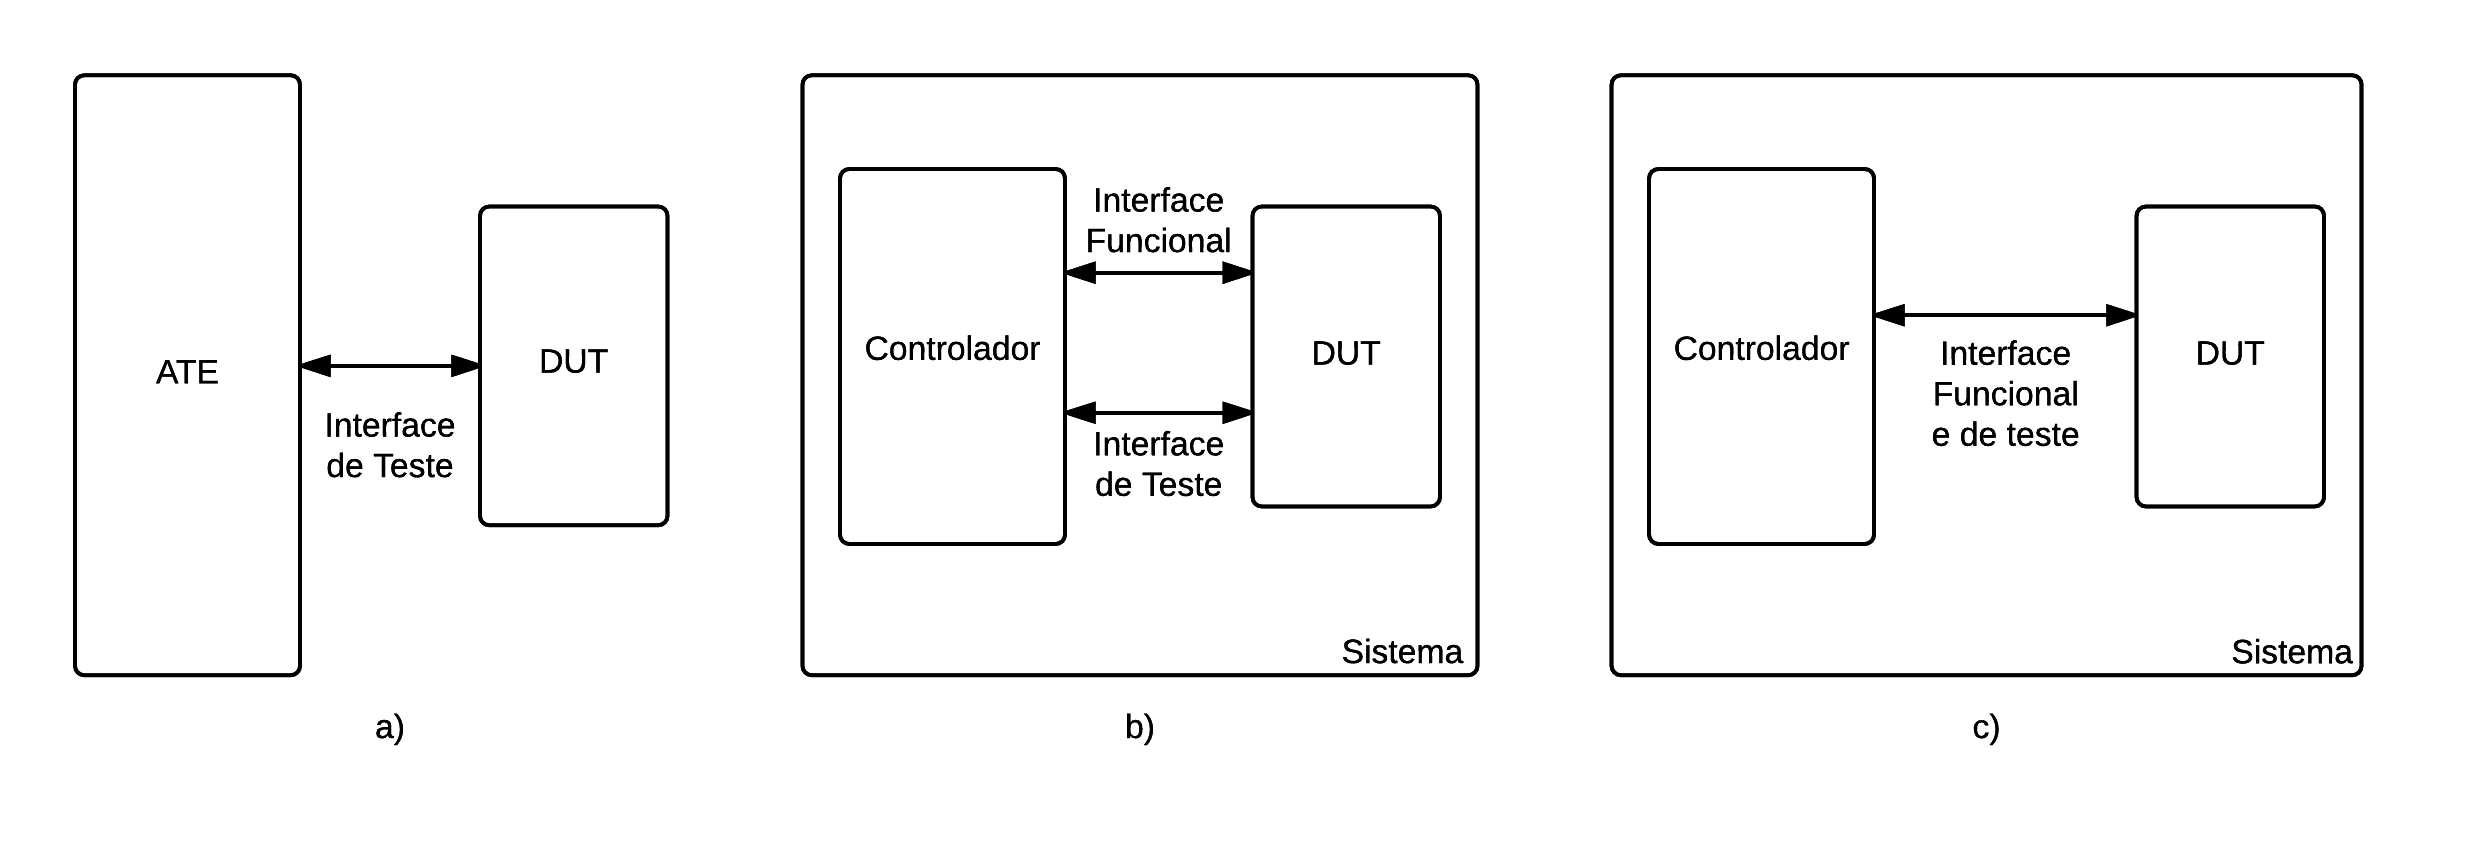
\includegraphics[width=1\linewidth]{tamreuse}
\caption{Reuso dos meios de acesso a teste. Retirado de Jutman (2014)}
\label{fig:tamreuse}
\end{figure}

\subsection{Dependência, proteção e segurança}
%rever toda essa parte pq n fez sentido
Segundo Jutman (2014), a abertura da infraestrutura de teste e diagnóstico vem também com um certo risco. É necessário garantir que esta infraestrutura não interfira na lógica do sistema e o acesso precisa ser restrito. Medidas de segurança precisam ser tomadas para garantir o acesso autorizado\citep{baranowski2013securing}.
A figura \ref{fig:mr} mostra diversas opções de restrição de acesso às RSNs.
\begin{figure}
    \centering
    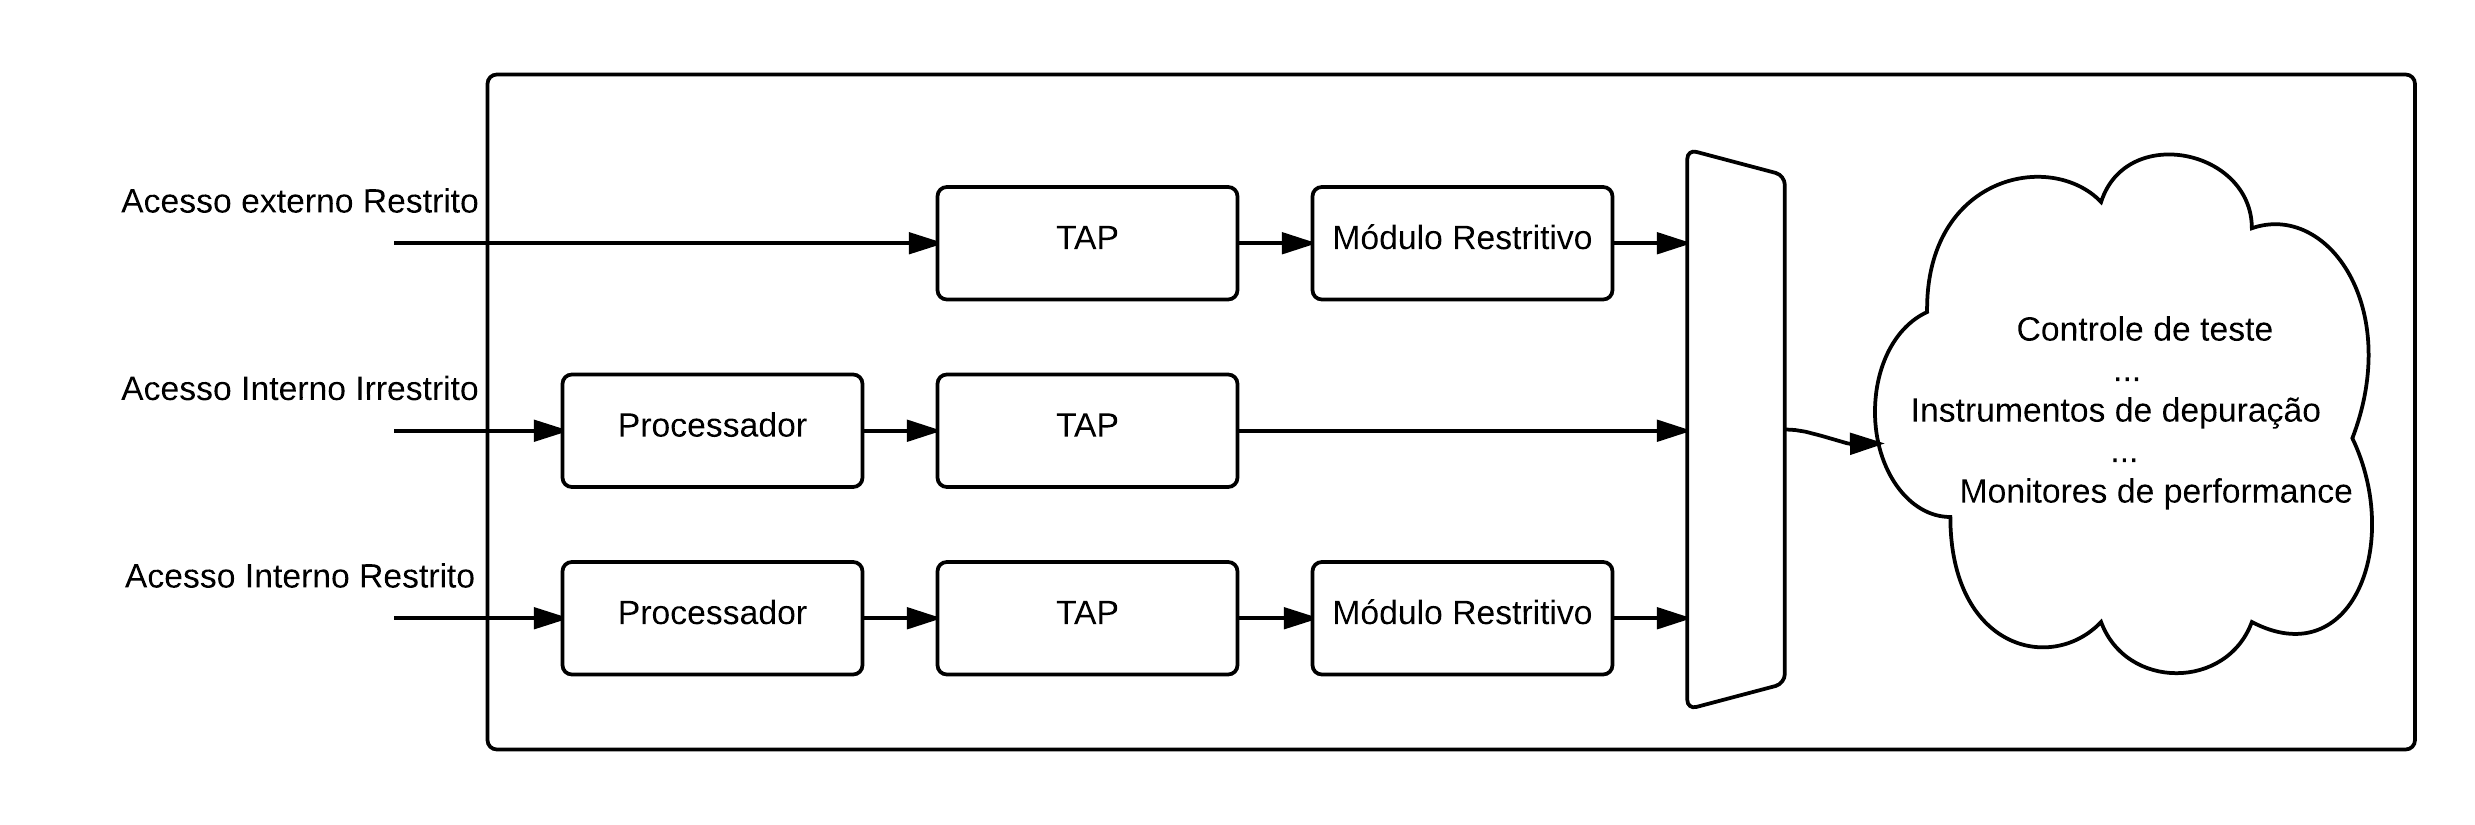
\includegraphics[width=1\linewidth]{mr}
    \caption{Restringindo acesso à infra de testes (Jutman et al., 2014)}
        \label{fig:mr}
\end{figure}
Jutman (2014) também apresenta como solução a introdução de um módulo restritivo (MR), que garante acesso para certas funcionalidades e estruturas de teste. Frequentemente, níveis diferentes de privilégios devem ser concedidos dependendo de autorização. Para a validação do sistema, análise de falhas de manufatura ou uma inspeção detalhada de retornos de campo, o acesso absoluto pode ser concedido. Numa oficina durante a manutenção, o acesso pode ser limitado para somente a coleta dos dados necessários para o reparo do sistema, e, para o usuário, pode-se somente permitir a coleta de checagens \textit{OK / Não OK}.

\subsection{Arquitetura \textit{on-chip} para diagnóstico embutido}
% a good reference for this http://eesemi.com/bist.htm
%https://en.wikipedia.org/wiki/Design_for_testing
%https://en.wikipedia.org/wiki/Automatic_test_pattern_generation
%

Como já mencionado, o auto diagnóstico embutido (BISD) concede o poder de pesquisa de faltas e defeitos sob às mesmas condições ambientais nas quais apareceram em campo sem que para isto seja necessário abrir ou obstruir o sistema. Entretanto, os esquemas BISD desenvolvidos para o teste durante a fabricação talvez não sirvam para o teste em campo, considerando as divisões do processo produtivo comparado ao contexto de operação em campo (Jutman et al., 2014). Se uma falta foi detectada durante a fase de autoteste, outras etapas adicionais são executadas para obter um diagnóstico intermediário e melhor localização da falta. \citep{cheng2007signature, wohl2002effective}\\

No caso de ASICS ou FPGAs, pode-se estender a arquitura STUMPS pela separação de três memórias: uma memória para os vetores de teste, outra memória de armazenamento de respostas para sinais intermediários, e uma memória de falha que armazena algumas assinaturas de falhas intermediárias, uma única etapa de teste é suficiente (ver figura \ref{fig:singlepass}).
\begin{figure}
    \centering
    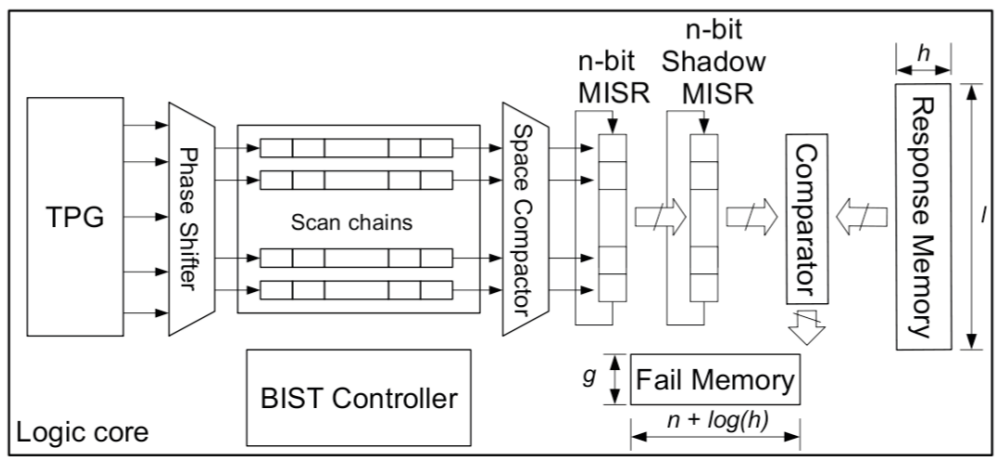
\includegraphics[width=1\linewidth]{bist}
    \caption{Esquema para um auto-diagnóstico embutido de passagem única (Jutman et al., 2014)}
    \label{fig:singlepass}
\end{figure}
O registrador MISR (Multiple Input Signature Register) coleta \textit{h} assinaturas intermediárias; cada uma delas é passada por um MISR "sombra" que roda alguns ciclos adicionais com a função de distribuir os últimos bits capturados uniformemente. As assinaturas corretas são armazenadas na memória de resposta e comparadas com as que foram capturadas. Em caso de diferenças, até no máximo \textit{g} assinaturas de falha, incluindo seus índices, são armazenadas na memória de falha. Assim, serão conhecidas até \textit{g} assinaturas de falha, e que as assinaturas entre elas estavam corretas. Essa informação é suficiente para computar potenciais falhas com alta resolução e precisão \citep{cook2014diagnosis}.

Apesar dos custos adicionais, o valor agregado do reuso dos esquemas de teste estrutural da manufatura do semicondutor para o teste e diagnóstico à nível sistêmico é notório. Ainda, assim como em testes de produção, não podemos confiar somente no teste estrutural como será discutido na próxima sessão.  
    %\chapter{O teste funcional no teste sistêmico}
%\addcontentsline{toc}{chapter}{O papel do teste funcional no teste sistemico}

	\section{Definições}
		Conforme \citet{jutman2014high}, diferentes definições existem para o conceito de "teste funcional". Uma abordagem entende como um teste que não depende de nenhuma estrutura DfT: dessa forma, este teste somente atua nas entradas funcionais do sistema, e somente observa as saídas funcionais do sistema.
		Em outra abordagem, um teste funcional é entendido como um teste que foi gerado somente para aproveitar as informações funcionais do sistema alvo (i.e., sem ter conhecimento de sua estrutura). Como consequência, este teste não depende de nenhum modelo de falha estrutural, levando a possíveis limitações na sua capacidade de cobertura de falhas.
		Mesmo assim, muitas vezes ambas as definições podem ser adotadas simultaneamente: por exemplo, um teste pode ser gerado começando pelas informações funcionais sobre o sistema, e o teste é aplicado pela reorganização de entradas e saídas funcionais.

	\section{Casos e motivações para o teste funcional}
		O teste funcional pode ser adotado em diferentes casos de teste funcional e pode ser motivado por diferentes razões. Ao tratar dos testes a nível de placa, o teste funcional é tipicamente considerado a etapa final (tabela \ref{tab:testcategories}), que supostamente é para complementar as etapas anteriores com objetivos especificos (e.g., testar as interfaces), permitindo atingir a cobertura de defeitos desejada. \citet{jutman2014high} cita exemplos adicionais do uso do teste funcional à nível sistêmico:
		\begin{itemize}
			\item Durante o teste de manufatura de um SoC, o teste funcional pode complementar o teste estrutural porque talvez possa cobrir alguns defeitos que não são detectados pelo último, e.g., porque o primeiro trabalha tipicamente em velocidades operacional (enquanto algumas técnicas DfT não), ou porque o teste funcional excita o sistema exatamente nas mesmas condições da fase operacional.
			\item Antes de montar um componente em uma placa, pode ser requisitado por regulações ou por conveniência econômica a execução de um teste para checar quando um dispositivo é livre de faltas (independente do teste executado pelo fabricante do dispositivo). Este teste (às vezes chamado de inspeção de recebimento ou \textit{incoming inspection}) é executado pelo fabricante do sistema e é frequentemente baseado somente na abordagem funcional -- até porque as possíveis funções DfT não são documentadas pelo fornecedor do dispositivo.
			\item Durante o teste em campo de uma placa, pode acontecer de que as funcionalidades DfT dos dispositivos que a compõe não estão mais acessíveis (e.g., porque requerem equipamentos de teste automatizado - ATE), ou porque não estão documentados pelo fornecedor dos dispositivos. Dessa forma, a única solução viável para a companhia OEM é frequentemente baseada em um teste funcional. Se o fabricante do componente não fornecer um teste adequado, uma rotina de teste funcional deve de ser desenvolvida começando pelas funções executadas por cada um dos componentes.
		\end{itemize}
	
	\section{Principios do teste funcional}
	
		Na maioria dos casos, um teste sistêmico funcional requer um programa de teste \textit{TP} apropriado para ser executado pelo(s) processador(es) dentro do sistema; espera-se que este programa de teste produza resultados diferentes quando o sistema estiver afetado por uma falta; resultados teriam de ser observados numa porta de saída apropriada ou corresponder a valores deixados em alguma área de memória especificada \citep{jutman2014high}. Quando o foco do teste forem os módulos periféricos, pode ser que seja necessário usar dados de excitação (\textit{TD}) apropriados em portas de entrada específicas, ou alguns dados de saída terá de ser observado em sinais de saída específicos.
		
		Quando o teste funcional é a solução escolhida, dois pontos principais precisam ser considerados \citep{jutman2014high}:
		\begin{itemize}
			\item Como aplicar o teste funcional, isto é, onde armazenar o programa de teste TP, como acionar o processador para executá-lo, como recuperar e checar os resultados produzidos; uma solução comum consiste primeiramente em armazenar o TP numa memória interna ( ou diretamente no cache do processador), acionando a sua execução por sinal de interrupção, e a partir daí checando os resultados na memória de dados (\textit{Software-Based Self-Test, ou SBST}) \citep{psarakis2010microprocessor};
			\item Como gerar o teste funcional (especificamente, o programa de teste TP).
		\end{itemize}
		Soluções para o primeiro assunto são tipicamente dependentes do sistema alvo e das restrições existentes. Para além disso, quando se lida com testagem em campo, a maioria destas tarefas são normalmente gerenciadas pelo Sistema Operacional.
		
		\section{Geração do teste funcional}
			A geração de programas de teste funcional adequados tem sido o objeto de pesquisa de diversas empreitadas de pesquisa, começando por \citet{thatte1980test}, onde os autores propuseram um método para gerar manualmente um programa de teste para um processador simples, conhecendo somente sua ISA (Instruction Set Arquiteture). Curiosamente, o método apresentou experimentalmente ser capaz de atingir uma boa cobertura de falhas (por volta de 90\%).
			
			Nas ultimas décadas, esta abordagem foi estendida para atingir núcleos de processador de maior (e crescente) complexidade, assim como para componentes específicos de sistemas embarcados, como memórias, componentes periféricos e redes de interconexão.
		\section{A geração de testes funcionais para processadores}
			Um bom panorama dos métodos direcionados para núcleos de processadores é reportado em \citet{psarakis2010microprocessor}. Mais recentemente, pesquisadores focaram em módulos específicos dentro dos núcleos dos processadores modernos, como as BPUs (\textit{Branch Prediction Units}), MMUs (\textit{Memory Management Units}), ROBs (\textit{Reorder Buffers}), e controladores de Cache, mostrando que na maioria dos casos é possível desenvolver programas de teste que garantidamente atingem uma alta cobertura de faltas, sem que seja necessário conhecer a implementação detalhada de tais módulos. O interessante é que, algumas destas faltas que afetam tais módulos não produzem resultados errados, mas forçam o processador a se comportar temporariamente de uma maneira diferente, tipicamente requisitando um tempo maior para completar a execução do progrmaa de teste (faltas de desempenho). A detecção destas falhas podem ser particularmente desafiadoras, já que requerem certos artifícios para observar o comportamento temporal do processador de um modo preciso \citep{hatzimihail2007methodology}.
			
			Esforços recentes se direcionaram para o desenvolvimento de programas de testes funcional para processadores multi-núcleos \citep{kaliorakis2014accelerated} e GPUs \citep{di2013software}.
			
			Os métodos acima correspondem principalmente a algoritmos, possibilitando que um engenheiro habilidoso manualmente escreva um programa de teste direcionado para um módulo especifico ou para um processador inteiro. Todavia, o esforço e tempo para alcançar este resultado podem ser significativos, e representam uma grande desvantagem da abordagem funcional. Esforços anteriores para automatizar este processo, baseados em simulação extensiva e técnicas evolutivas \citep{corno2004automatic}, por exemplo, tiveram sucesso limitado, principalmente devido ao grande esforço computacional que elas requerem. Recentemente, foi mostrado em \citet{riefert2014effective} que técnicas formais podem ser exploradas com sucesso para gerar automaticamente programas de teste funcional para um processador com \textit{pipeline}.
			
		\section{A geração de testes funcionais para memórias}
			Considerando que as memórias correspondem à uma grande - e cada vez maior - parte de um sistema, seu teste podem representar um foco importante de teste. Todavia a solução típica depende da adoção de BIST, existem casos onde a abordagem funcional é também de interesse. Nestes casos a solução tradicional reside no desenvolvimento de um programa de teste que performa nos módulos de memória alvo a mesma sequencia de operações de leitura e escrita determinadas por um dado algoritmo de \textit{March}. A principio, isto garante que a mesma cobertura de defeitos é alcançada, ainda que alguns defeitos possam passar desapercebidos devido ao tempo maior entre dois acessos consecutivos às memórias \citep{van2010memory}. Uma extensão interessante da mesma ideia permite transformar testes de reordenação de memórias cache em programas escritos sob medida: \citet{di2011software} propõe um conjunto de regras que permitem transformar automaticamente qualquer algoritmo \textit{March} em um programa de teste correspondente. Já a referência \citet{riga2012functional} estende a mesma abordagem para as memórias cache L2.
		\section{A geração de teste funcional para periféricos e interconexões}
			Ao focar componentes periféricos de comunicação, a abordagem funcional requer a ação combinada do processador, programando o componente e excitando-o/observando-o de um lado, e de um corpo externo (um ATE, por exemplo), excitando/observando o componente a partir do outro lado do canal de comunicação \citep{apostolakis2009test}. Para soluções em campo, onde o ATE dificilmente possa ser usado, uma conexão \textit{loop-back} é frequentemente adotada. Uma abordagem similar pode ser adotada para periféricos do sistema, como controladores de Interrupção e DMA \citep{grosso2012software}.
			
			Vários métodos tem sido propostos para desenvolver um teste funcional capaz de efetivamente detectar faltas nas estruturas de interconexão dentro de um sistema. Como um exemplo, o trabalho em \citet{dalirsani2014structural} foca em faltas estruturais em um NoC (\textit{Network on a Chip}).
		\section{Tópicos Ativos na área de Teste Funcional}
			Na ultima década, foram desenvolvidos métodos para gerar programas de teste funcional sob restrições especificas (e.g., in termos de energia \citep{zhou2006software}) ou provendo informação de diagnóstico \citep{bernardi2008effective}.
			
			Tanto a academia quanto a indústria estão explorando os custos e benefícios da integração da abordagem funcional com um suporte de hardware limitado, como proposto em \citet{bernardi2010exploiting} e \citet{reimann2014advanced}. Ao focar teste de placas, o reuso de instrumentos embarcados e FPGAs on-board (como citado na sessão \ref{advPCBA}) também estão sendo exploradas; 
			Por fim é importante mencionar que ao direcionar arquiteturas de processador mais comuns, como aquelas com processadores VLIW\footnote{\textit{Very Long Instruction Word}}, é possível adotar uma abordagem hierárquica, na qual o programa de teste global pode ser construído, assim que cada unidade que o compõe for conhecida \citep{sabena2012automatic}. Dessa maneira a maior desvantagem da abordagem funcional, correspondendo ao grande custo de gerar manualmente o teste (como uma consequência da falta de ferramentas automatizadas), pode ser encarada.
			
			Seguindo esta abordagem, esperam-se novas empreitadas no futuro próximo, focados na automatização da geração de programas de teste funcional (para ser adotados em diferentes cenários) explorando certas informações vindas do núcleo ou fabricante do dispositivo, assim como do projetista do sistema.
			
			


\part{O experimento}
        \chapter{Estudo de caso e metodologia}
%\addcontentsline{toc}{chapter}{Estudo de caso e metodologia}
        Esta sessão descreve o dispositivo a ser testado, assim também como a metodologia utilizada para abordar a modelagem de software.



\section{O dispositivo sob teste e sua jiga}

        Como mencionado no capítulo \ref{intro}, o escopo de desenvolvimento foi reduzido a um único produto como forma de simplificação de projeto. Considerando isto, escolheu-se o GT650\footnote{\citep{v2com2016}}, que é o produto principal da empresa. Projetado para atender demandas de distribuição de energia, o GT650 é um módulo de comunicação móvel para gerenciamento de medições automatizadas controle de redes de transmissão e distribuição. Sua PCIM pode ser vista nas figuras \ref{fig:board} e \ref{fig:board_inf}.
        
        \begin{figure}
            \centering
            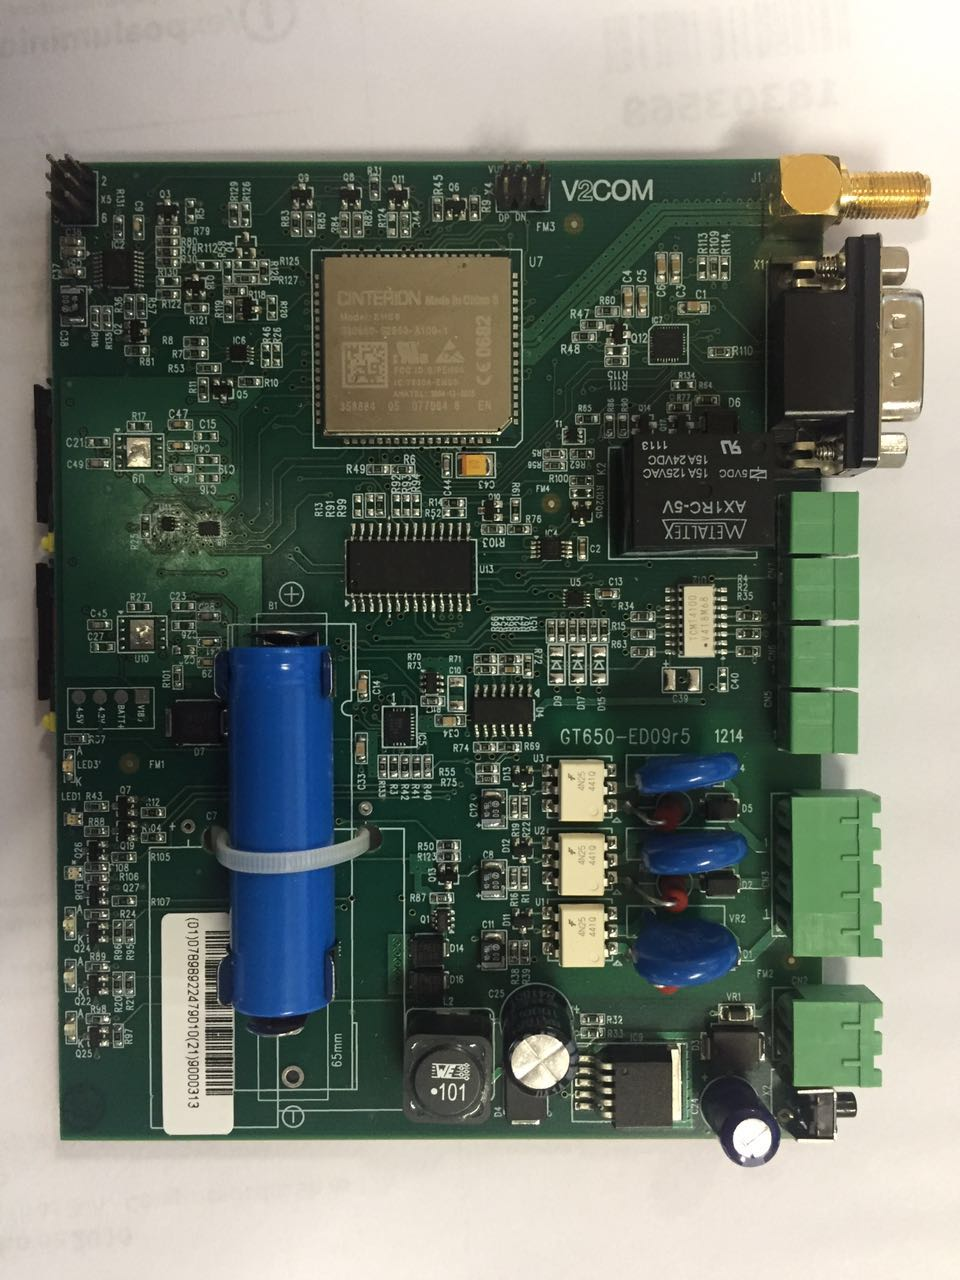
\includegraphics[width=0.9\linewidth]{board}
            \caption{foto do lado superior  do GT650}
            \label{fig:board}
        \end{figure}
        
        \begin{figure}
            \centering
            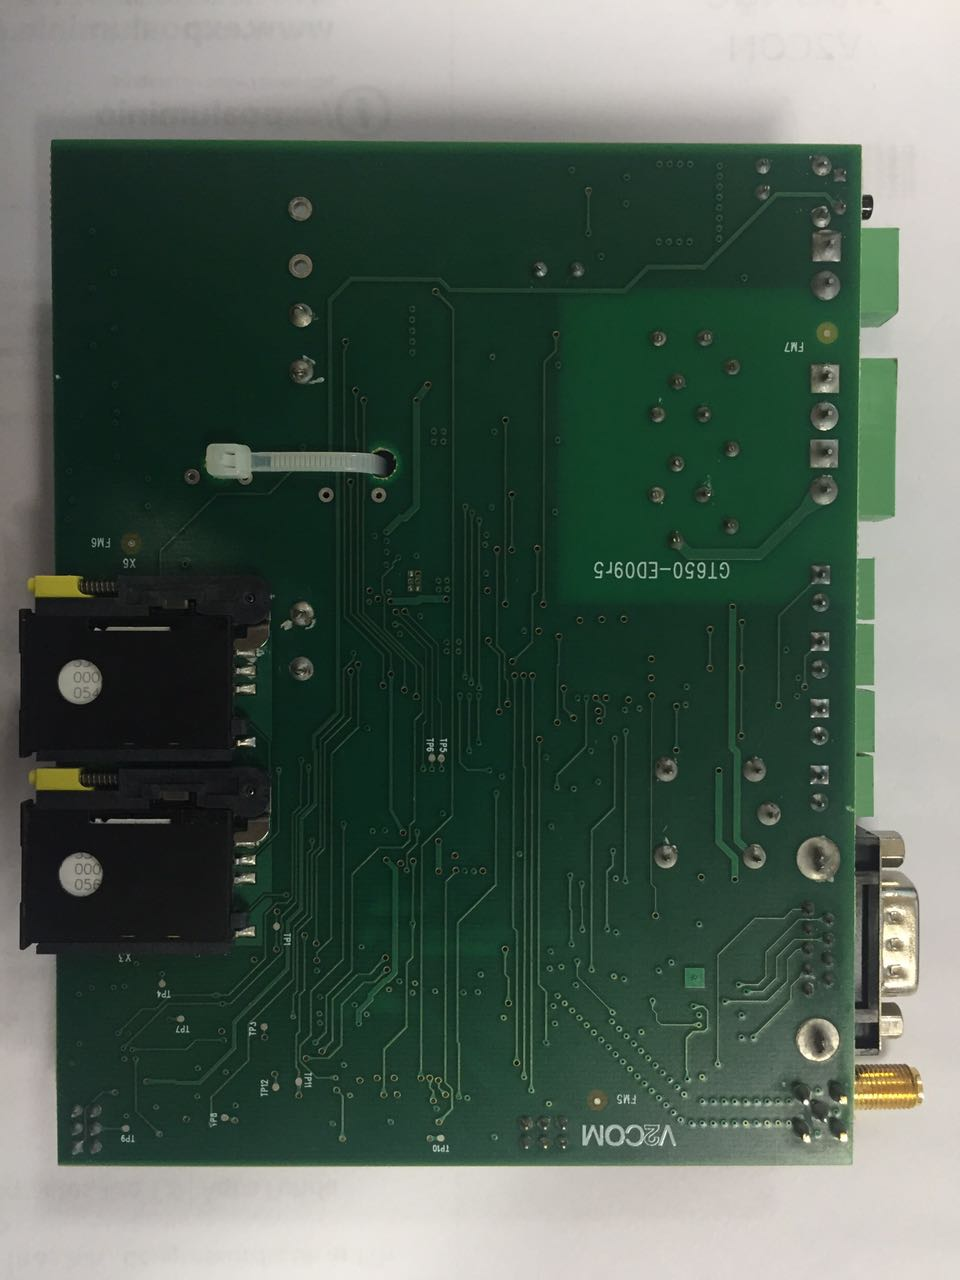
\includegraphics[width=0.9\linewidth]{board_under}
            \caption{foto do lado inferior  do GT650}
            \label{fig:board_inf}
        \end{figure}
        
        Segundo o site da empresa, o GT650 serve como um módulo integrável à qualquer religador, medidor de energia, ou dispositivo de distribuição, por diversos protocolos, sendo RS-232 e Ethernet os mais utilizados. 
        Seu software embarcado pode ser atualizado remotamente via OTAP (over-the-air provisioning\footnote{over-the-air provisioning é um método de atualização de software remotamente. Isso é normalmente implementado no próprio bootloader do sistema \citep{jacobbeningo2013}.}) e sua operação continua é assegurada por uma bateria de lítio embutida. Além disso o módulo possui sensor de tensão trifásica para detecção de anormalidades, e portas digitais para detectar a abertura de gabinetes ou qualquer outra customização que o cliente solicitar.
        
        \begin{figure}
            \centering
            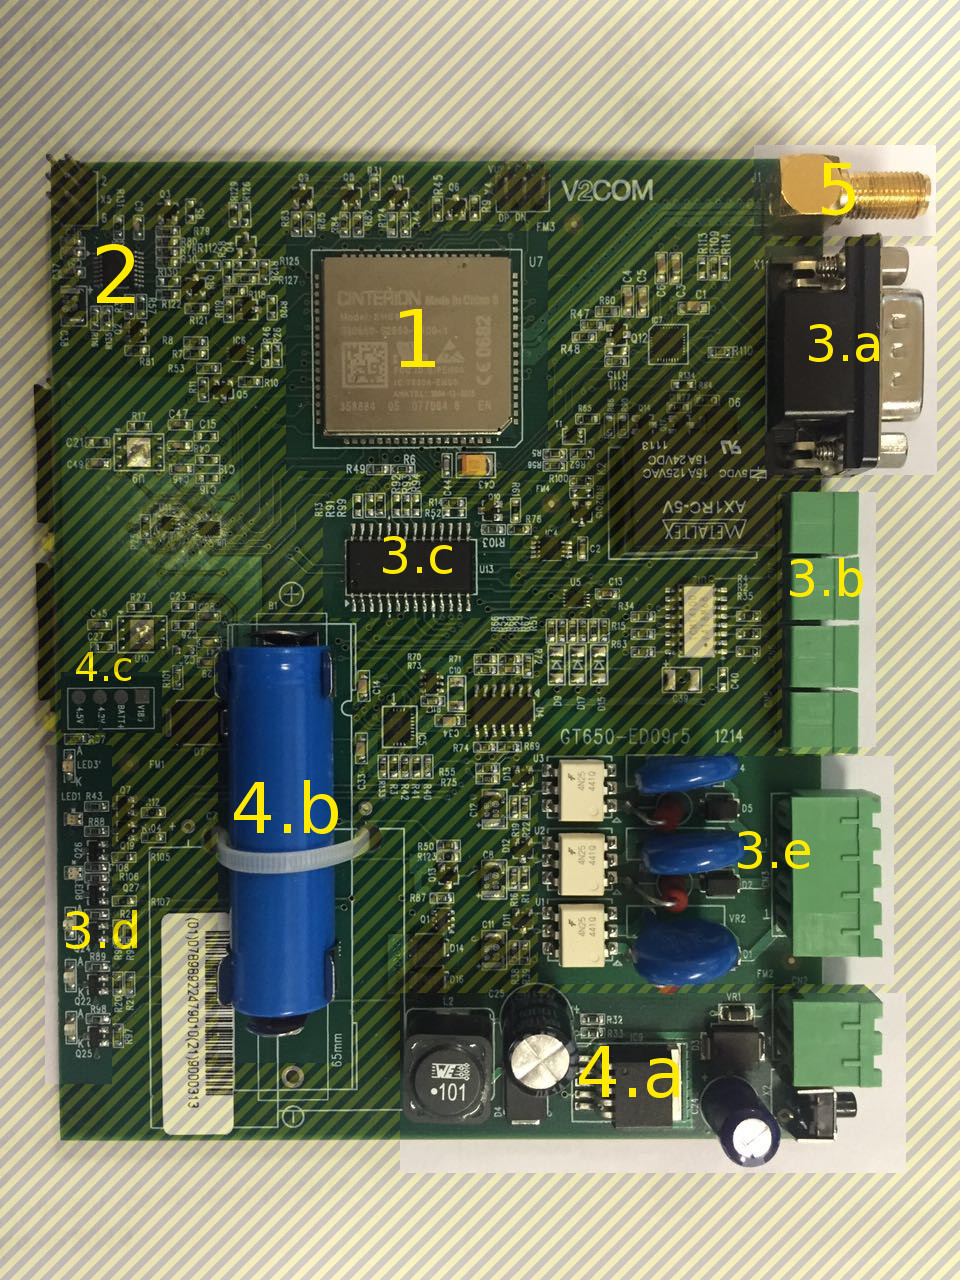
\includegraphics[width=0.9\linewidth]{placa}
            \caption{foto do GT650 com destaque aos componentes da placa}
            \label{fig:placa}
        \end{figure}
        
            \subsubsection{Módulo M2M}
                O processador principal da placa é o modem EHS6 da  Cinterion (ponto 1 da figura \ref{fig:placa}), que segundo o site do fabricante, contém: %todo cite EHS6 DATASHEET
                
                \begin{itemize}
                    \item Cinco bandas de 3G (HSPA): 800/850/900/1900/2100 MHz
                    \item Quatro bandas GPRS/EDGE Class 12: 850/900/1800/1900 MHz
                    \item Suporte a Java™ ME\footnote{Java Micro Edition é  uma plataforma Java para sistemas embarcados} 3.2, com suporte a multi-threading e execução de múltiplas aplicações, além de 6 MB de memória RAM e 10 MB de memória Flash;  %todo cite JAVA ME
                    \item Pilha de protocolos TCP/IP embarcada e acessível por comandos AT, incluindo conexão segura via TLS/SSL; serviços DNS e Ping; Cliente FTP e HTTP; %todo cite AT Commands
                    \item Interface USB 2.0 HS, e duas portas de interface modem serial;
                    \item 16 GPIOs compartilhadas com as portas de comunicação, PWM, etc.
                    \item ADC e interface I$^{2}$C 
                    \item Atualização de \textit{Firmware Over-the-air} (FOTA)
                \end{itemize}
                
                Basicamente é o componente central do produto: Comunicação TCP/IP via GSM/3GPP/GPRS; Aplicações Java, interface serial com o mundo externo e I$^{2}$C com os componentes periféricos da placa.
                
                O fabricante não fornece informações internas sobre a arquitetura, como também nenhum meio de acesso à estrutura interna do módulo. Como contrapartida a empresa oferece garantia de funcionamento, assim como suporte técnico completo.
                
                Todavia, isto impede testes estruturais e verificações mais profundas nos módulos, tanto na produção, quanto na manutenção e torna todos os processos dependentes de agentes externos. O teste estrutural se limita a verificação de interconexões do componente com a placa. Como já mencionado este teste é realizado pela empresa responsável pela montagem e é realizado através de equipamentos de AXI -- \textit{caso a contratada possua} -- Pois o encapsulamento LGA impossibilita conferir visualmente, ou por AOI, todas as interconexões. 
                
                Todo e qualquer problema que ocorrer com estes módulos, seja físico ou de \textit{firmware}, é enviado ao fabricante original para solução, muitas vezes dependendo do suporte na Alemanha. Por um lado, é positivo já que tira da empresa, a responsabilidade de resolver problemas de baixo nível, assim como a necessidade de manter pessoal e equipamento especializado para analisar este tipo de problema. Por outro lado, trabalhar com componente e \textit{firmware} fechados deixa a produção sujeita a problemas invisíveis. Um erro de \textit{firmware}, por exemplo, poderia ocasionar um \textit{recall} de um lote inteiro.
                
                Por estas limitações no teste estrutural, o escopo de teste fica restrito às verificações funcionais, principalmente através de comandos AT, como veremos na sessão \ref{metodologia}. 
                
            \subsubsection{Monitor \textit{Watchdog}}
                Este componente é um microcontrolador simples de 8 bits (figura \ref{fig:placa}, no ponto 2), e é  responsável por desligar o modem por duas maneiras: a primeira pelo temporizador watchdog, e a segunda pelo botão liga-desliga. 
                
                Também é armazenado nele o número de série da placa. Dessa forma a empresa consegue separar o rastreamento dos \emph{modems} e das \emph{placas}, podendo intercambiá-las conforme necessário.
                
                No escopo de teste algumas coisas foram elencadas pela equipe: conferir o número de série, teste do botão liga-desliga, e teste do temporizador \textit{watchdog}.
                
            \subsubsection{Interfaces cabeadas e com o usuário}
                Por ser uma solução de comunicação para outros equipamentos, o GT650 não possui interfaces digitais e analógicas muito complexas, exceto pela comunicação de dados via GSM, que será descrita à parte. Como pode ser visto na figura \ref{fig:placa}, a placa possui:
                
                \begin{itemize}
                    \item Duas portas RS232 (\ref{fig:placa}-3.a);
                    \item Três portas de entrada digitais opto isoladas (\ref{fig:placa}-3.b); 
                    \item Um relé de saída (\ref{fig:placa}-3.b);
                    \item Seis LEDs de sinalização (\ref{fig:placa}-3.d);
                    \item Uma porta para conferência de tensão trifásica (\ref{fig:placa}-3.e);
                \end{itemize}
                
                Vale mencionar que as entradas e saídas digitais, assim como os LEDs são controlados pelo modem atrávés do expansor de GPIO (\ref{fig:placa}-3.c) por endereçamento I$^{2}$C.
                
                Assim como nos pontos anteriores o escopo de teste se limita a verificações funcionais.
                
            \subsubsection{Alimentação, bateria e BMS}
                O sistema de alimentação consiste em um conversor CC-CC de 12 Volts com saídas de 3.3 Volts e 5 Volts (figura \ref{fig:placa}-4.a), e uma bateria de lítio de 4.8 Volts para em caso de faltas na rede (figura \ref{fig:placa}-4.b). 
                
                Para testar este sistema, foram criados quatro pontos de teste na placa como vistos no ponto 4.c da figura \ref{fig:placa}: 5V, BATT+, 3V3, e 1.8V. Atualmente, o teste é realizado manualmente com o multímetro, ponto por ponto, mas enviando os dados de leitura pelas portas seriais de computador. Pretende-se automatizar esta etapa nas próximas revisões da jiga de testes.
                
            \subsubsection{Comunicação GPRS/EDGE/UMTS}
                A comunicação de dados por UMTS é a interface principal do módulo e opera nas bandas: 800, 850, 900, 1900 and 2100 MHz. Além disso suporta dois cartões SIM.
                
                Originalmente, este sistema era testado por um simples teste de comunicação, mas devido a problemas de queda de potência de sinal causados por solda mal feita, que só apareciam em campo, esta estratégia foi substituída. Atualmente é usado um medidor de potência RF -- O \emph{NI USB-5680} -- que tem uma faixa de frequência 50 MHz até 6 GHz, alcance de potência de -40 a +23 dBm, e uma banda de canal 10 a 100 MHz. Esta nova estratégia adotada, praticamente eliminou os retornos de campo por problemas de alcance do produto.

    \subsection{O que é testado e o que precisa ser testado}
        
        
        O roteiro de teste anterior a este trabalho consistia no teste sequencial das funcionalidades da placa, ou seja um teste funcional. Conforme mencionado na sessão anterior, pela própria ausência de uma porta JTAG ou outra forma de acesso interno, e também por não ter nenhuma lógica programável no produto, o teste estrutural se limita à verificação ótica ou radiográfica das interconexões das PCIM. 
        
        Neste trabalho, decidiu-se por reproduzir o mesmo roteiro de teste utilizado anteriormente para não causar impactos negativos na rotina da produção da empresa. 
        
        É importante notar que este roteiro é ainda bastante sequencial, abrindo a possibilidade de otimização com rotinas concorrentes no escopo de teste. Isto será descrito na sessão \ref{metodologia}, que trata da metodologia e especificação de software.
        
        
        %todo anexar roteiro anterior?

    \subsection{A Jiga de teste}
        
        A decisão da equipe de engenharia foi utilizar a jiga de testes corrente, e foi atribuído a um projetista de hardware da equipe a tarefa de especificar e desenvolver uma nova plataforma de teste. 
        
        Este foi um ponto considerado nas especificações do programa que serão vistas na seção \ref{metodologia} do presente trabalho. 
        
        Esta Jiga é basicamente testes de interface, não possuindo nenhuma ponta de teste ou algo que se aproxime de uma \emph{cama de pregos} de teste para testes mais internos.  
    
        A Jiga possui comunicação serial do DUT com o computador, assim como um ponto de conexão do aterramento da placa com o negativo do multímetro e sua comunicação serial com o PC. Também permite ao operador fixar níveis lógicos alto ou baixo nas portas digitais, assim como tensões trifásicas na porta trifásica.
    
    \section{Metodologia e especificação de Software} \label{metodologia}

    \subsection{Levantamento de Requisitos}
        Requisitos são objetivos ou restrições estabelecidas por clientes e usuários que definem as diversas propriedades do sistema. Os requisitos de software são, obviamente, aqueles dentre os requisitos do sistema que dizem respeito às propriedades de software. Tradicionalmente, eles são divididos em \textit{funcionais e não funcionais}.
        
        Requisitos funcionais são a descrição das funcionalidades que o programa deve oferecer. E é genérico no sentido que não necessariamente trata-se de interações com o usuário, mas também como funcionalidades ocultas como, por exemplo, uma API, interações com hardware, e comunicação \citep{bourque2014guide}.
        
        Requisitos não-funcionais são qualidades globais de um software como manutenibilidade, usabilidade, desempenho, custo e vários outros. Normalmente estes requisitos são descritos de maneira informal, de maneira controversa (certos objetivos são concorrentes um com o outro) e são difíceis de validar\citep{bourque2014guide}.
        
        A partir do cenário estudado anteriormente, foram levantados os seguintes requisitos não-funcionais:
        \begin{itemize}
            \item O programa deverá ser implementado em LabVIEW;
            \item Reusabilidade de código;
            \item Concorrência e paralelismo do roteiro de testes;
            \item Modularização dos testes e do roteiro;
            \item Interface de usuário ergonômica e intuitiva;
        \end{itemize}
        
        Já os requisitos funcionais consistem no roteiro de testes anterior a este trabalho, conforme decisão da equipe de engenharia de fábrica:
        \begin{itemize}
            \item Leitura e armazenamento do número de série colado na placa por um leitor de código de barras;
            \item Comunicação com o DUT via serial;
            \item Teste das duas portas seriais;
            \item Verificar se o modelo de modem é o EHS6;
            \item Verificar se a \textit{firmware} do modem é a mais atual;
            \item Armazenar o IMEI\footnote{\textit{International Mobile Station Equipment Identity} ou Identificação Internacional de Equipamento Móvel é um número de identificação global e único para cada telefone ou modem celular.} do modem;
            \item Configurar as GPIOs do modem conforme o perfil da aplicação;
            \item Abertura, seleção e teste das duas bandejas de cartão SIM\footnote{\textit{subscriber identity module}};
            \item Configurar e testar comunicação $I^{2}C$;
            \item Configurar operação do expansor de IO, MCP23018: interrupção espelhada, não incremento de ponteiro, interrupção push-pull;
            \item Configurar e testar do BQ24070, carregador de bateria e \textit{system power-path} do sistema;
            \item Teste de leitura da bateria;
            \item Teste do microcontrolador de watchdog (MC9S08QG8), e do botão liga e desliga;
            \item Leitura do número de série armazenado no MC9S08QG8, e validação deste com o número de série colado  na placa;
            \item Teste de comunicação e leitura do sensor de temperatura LM75
            \item Teste de morte de sessão;
            \item Testes dos barramentos de tensão da placa: 4.5V, 4.2V, BATT++, e 1.8V;
            \item Teste do painel de LEDs;
            \item Teste de detecção de retirada e inserção da fonte de alimentação;
            \item Teste das 3 portas digitais;
            \item Teste de acionamento e desarme de relé;
            \item Teste da porta de tensão trifásica - detecção de presença e ausência;
            \item Teste de interrupção de desligamento e reset da placa;
            \item Ainda que não presente no roteiro da linha de produção ( esta etapa é realizada posteriomente), possibilidade de teste de potência de sinal de transmissão HSPA;
            \item Geração de arquivos de log de teste em .txt;
            \item Notificação para o operador sobre sucesso ou falha do teste, assim como possibilidade de reteste.
        \end{itemize}
    Passado o levantamento de requisitos, a etapa seguinte foi a escolha de método de desenvolvimento, assim como as etapas do mesmo.
        
\begin{comment}
    \subsection{Workflow do projeto} % jeitinho de trabalhar
       
       Para a realização deste trabalho dentro da empresa, optou-se por um desenvolvimento incremental a partir de uma solução minimamente funcional. O projeto foi realizado em etapas, em ciclos curtos de desenvolvimento que pudessem ser entregues para receber a contrapartida da empresa e ser validado. Algo próximo da metodologia Agile. Esse processo permitiu uma maior interatividade entre as necessidades da aplicação, como forma de repensar a escopo do programa, e também facilitou o acompanhamento da gerência com o andamento do produto.
       
 %   \subsection{Síntese dos requisitos ambientais de teste}
% #todo

Validação do projeto
Controle de Qualidade
Melhorias de processos
Melhorias no produto
Auxilio na Manutenção
\end{comment}    
    \chapter{Modelagem e Implementação}
    \section{Modelagem}
        
        %  entendemos o contexto do problema, levantamos requisitos, agora vamos modelar e tentar aplciar padro~eos de projeto pra facilitar
        
        Ao compreender o problema e suas limitações e especificidades, pode-se partir para modelar uma solução para tal.
        
        É uma prática comum no desenvolvimento de software aplicar padrões de projeto, mais conhecidos como \textit{Design Patterns}, ou basear-se em alguma estrutura pré-estabelecida como fundação do desenvolvimento.
        %todo cite design patterns 
        
        Dessa forma, optamos por usar um framework já bem consolidado: O Actor Framework, que é a implementação do modelo de atores em Labview. Isto será melhor descrito logo abaixo.
        
        Outro ponto importante desta etapa é saber representar o modelo desenvolvido. Em engenharia de software, a ferramenta mais utilizada neste processo é a Linguagem de Modelagem Unificada (do inglês \textit{Unified Modeling Language ou UML}, que nos permite representar o sistema de forma padronizada.
        
                
    \section{Um proposta do sistema dentro do modelo de atores}     
        A configuração de atores e responsabilidades propostas podem ser vistas na figura \ref{fig:modelo}. 
        
        Separamos em cinco classes de atores: comunicação serial; ator de multímetro; gerador de arquivo de registro de teste; Teste de powermeter; e controlador.
        \begin{figure}
            \centering
            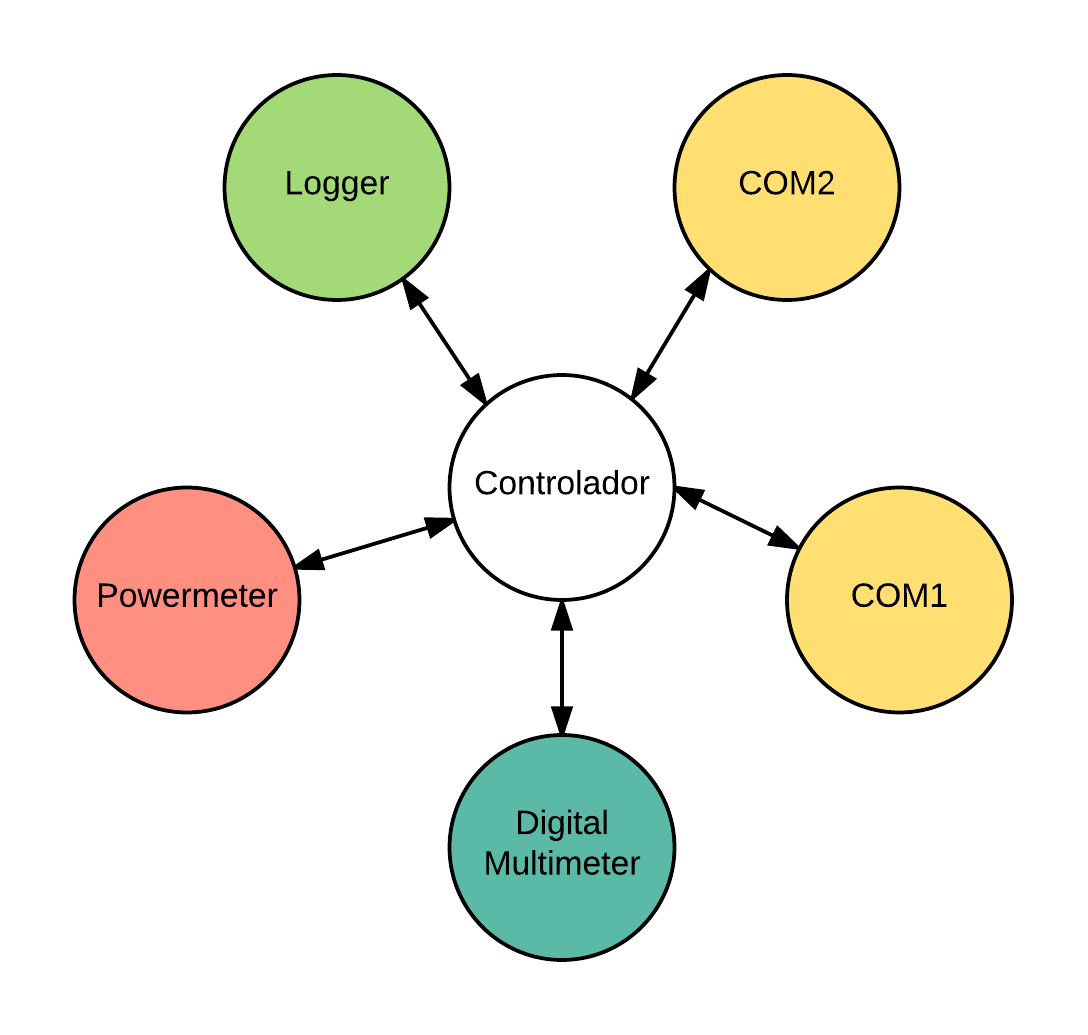
\includegraphics[width=0.9\linewidth]{fig/sistemmodel}
            \caption{Modelo do sistema no framework de atores}
            \label{fig:modelo}
        \end{figure}
            
        \subsection{Ator de comunicação serial}
            Ator responsável por enviar comandos de teste e verificar as respostas recebidas do dispositivo sob teste.
            
            Usamos dois atores no sistema pois trabalhamos com duas portas: uma para comunicar com o módulo por comandos AT, e outra para acessar periféricos conectados no barramento  I$^{2}$C. 
            
            Toda resposta aos comandos é verificada e relatada ao Ator Controlador, que por sua vez decide o fluxo de execução do roteiro de teste. 
            
            Devido ao curto prazo dado ao projeto, nessa implementação inicial não foi implementado o interpretador para o padrão de roteiros utilizados no programa anterior. o que daria bastante flexibilidade à equipe para editar o roteiro conforme mudanças de \textit{firmware}, aplicação ou revisões de placa. Ao invés disso, todos os comandos são parte do código fonte do programa, situação conhecida como \textit{hardcoding}. No contexto desse projeto isto é considerado um antipadrão de projeto de software, já que assumimos que variável ambiental é constante. %todo cite anti patterns
        \subsection{Ator Multímetro}
            \label{dmmmodel}
            
            Esta entidade é responsável pela leitura da porta RS232 do multímetro e transformar essas leituras em informações com mais sentido, e em uma interface de usuário ergonômica para o operador. Além disso, é interessante que o ator receba os vetores de teste para validar com as medidas.
            
            O multímetro utilizado é um ICEL MD-6400, com suporte de comunicação por uma porta serial RS232. A figura \ref{fig:dmmprotocol} exibe o funcionamento de seu protocolo, que a cada 250 ms, envia pacotes de 14 bits de dados a 9600 baudrate. 
            
            Logo, as primeiras etapas do algoritmo do multímetro seria ler e sincronizar os dados lidos pela porta serial. A sincronização é facil de implementar por meio de uma máquina de estados. Já a parte de decompor os dados do \textit{bitstream} em informação inteligível, vai desde a transformar números em código de sete segmentos em inteiros, a asssociar unidades de medida.
            
            Outra funcionalidade importante seria a de indicar o uso de um modo de operação incorreto, como por exemplo uso do instrumento como ohmímetro quando a medida era de tensão.
            
            Conforme mencionado no levantamento de requisitos do programa, são feitas quatro medições de tensão na placa. Os vetores de teste possuem os seguintes atribuitos: \textit{limiar máximo; limiar mínimo; unidade de medida; quantidade de novas tentativas permitidas}.
            
            Na sessão de implementação, será mencionado as melhorias na ergonomia do operador.
            
            \begin{figure}
                \centering
                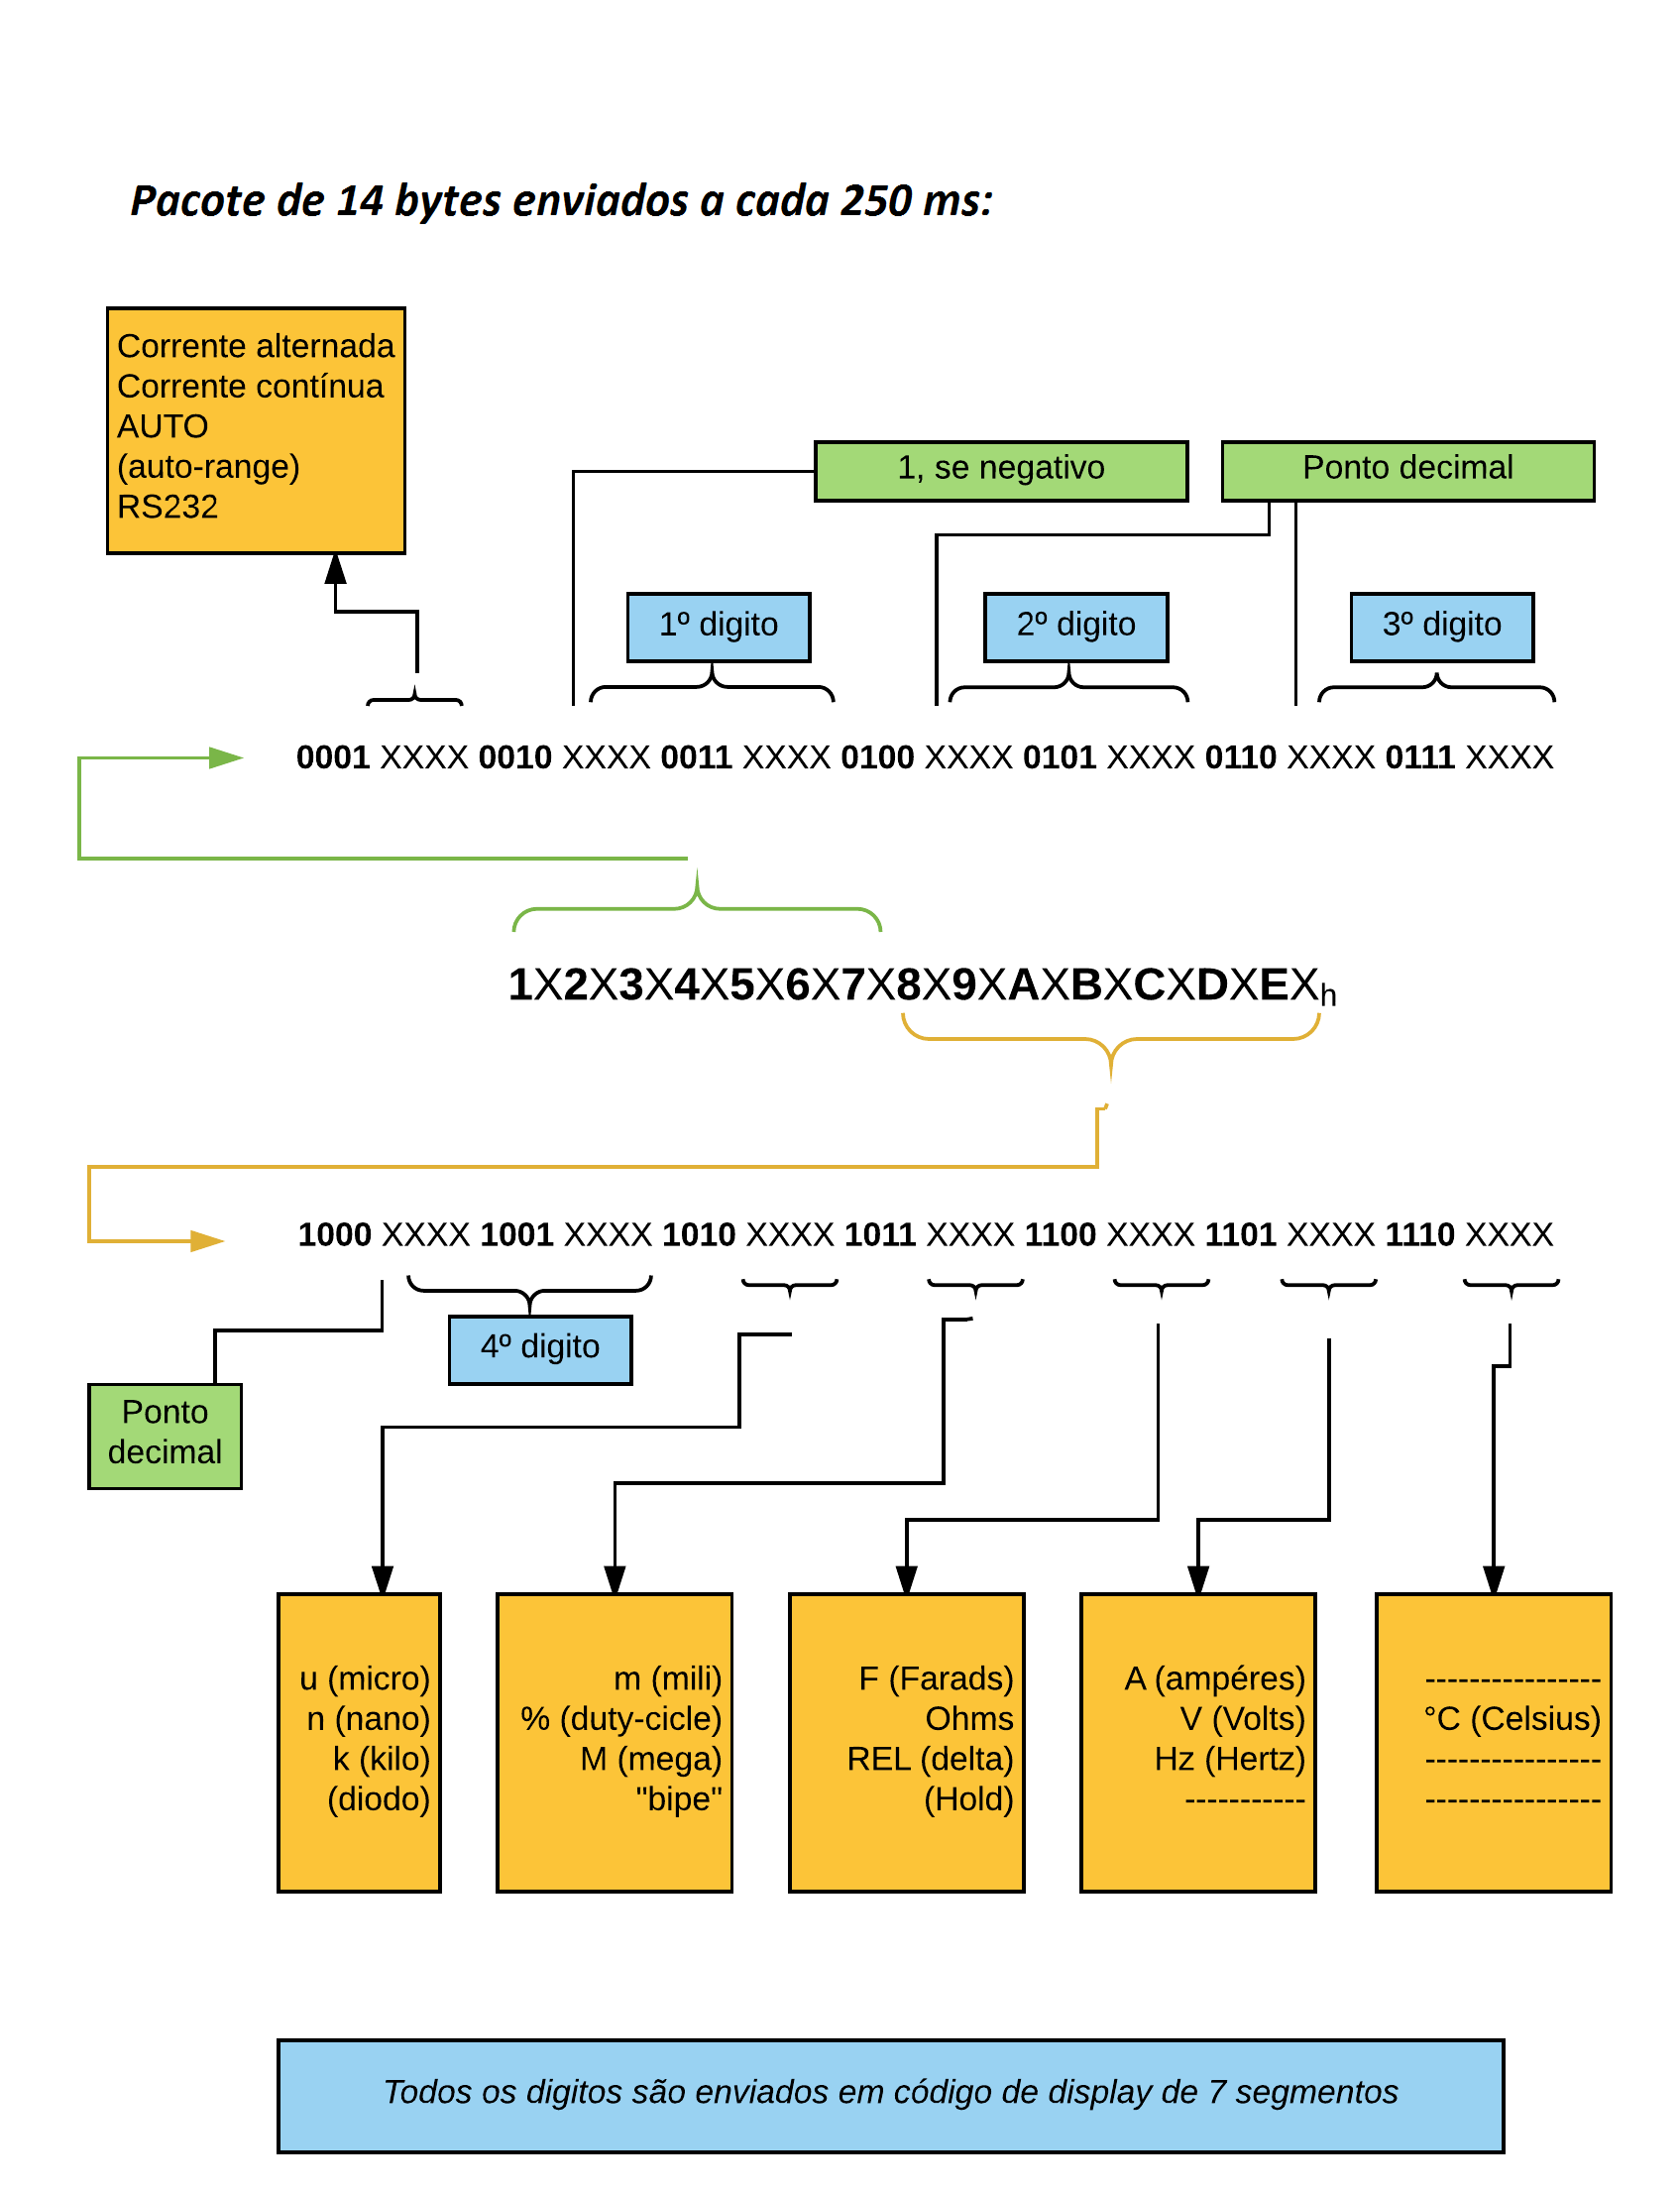
\includegraphics[width=\textwidth]{model/dmmprotocol}
                \caption{Protocolo de comunicação do multímetro}
                \label{fig:dmmprotocol}
            \end{figure}
            
        \subsection{Gerador de arquivos de registro}
        
            A saída principal do programa são os arquivos de registro, e para esta função foi designado um ator separado. 
            
            Dentre as suas funções estão: gerar um arquivo de registro completo do teste para fins de depuração e diagnóstico; gerar um arquivo de registro resumido só para o controle de qualidade em produção, e envio do registro para a base de dados dos produtos da empresa. E paralelo a isto foi desenvolvido um novo servidor de registros de teste com uma API própria.
            
            Este ator é alimentado pelo Controlador com informações do teste para preencher o arquivo de registro. 
            
        \subsection{Teste de potência do \textit{front-end}}
            \label{pwmodel}
        
            Ator que detém o controle do medidor de potência RF, também referenciado como \textit{Powermeter}. Este ator recebe como parâmetro a frequência de medição, o número de medidas, e os limites máximos e mínimos de de potência tolerados.
            
            O instrumento de medição de potência RF utilizado foi o NI 5680, da National Instruments, que mede potência RMS de sinais até 6 GHz, em larguras de banda bem estreitas (10-100 Hz de banda), e um alcance de potência de -40 dBm a +23 dBm.
            
            As baterias de testes estruturais e funcionais são quase todas realizadas dentro das empresas que realizam a montagem de placas, porém, o alto custo, a empresa possui só uma unidade deste instrumento, utilizado alternadamente entre o setor de manutenção e no final de produção. Por isso, a etapa de medição de potência de front-end é feita separada do demais testes e ainda não foi introduzida neste programa. 
            
            Para contornar isso foi feito um programa separado responsável por este teste, realizado no fim de linha de produção, antes de embalar o produto. E no programa deste trabalho, foi inserido a estrutura básica para implementação do medidor de potência de front-end.
            
        \subsection{Controlador}
            
            O controlador, como o próprio nome define, detém a responsabilidade sobre o fluxo de execução do programa, criando e destruindo os outros atores-módulos e fazendo a comunicação entre seus atores filhos. Além disso, detém a interface de usuário principal do programa. 
    
    \section{Modelagem UML}
        
        Para ilustrar o modelo do sistema estabelecido, foi escolhido representá-lo por um diagrama em linguagem universal de modelagem - UML, que é uma linguagem de uso geral dentro da engenharia de software, cuja a intenção é providenciar uma maneira padrão de representar o projeto de um sistema.
        
        \begin{comment}
        
        O padrão UML possui duas categorias de representação de software: Estrutural e Comportamental. Dentro dela temos:
        
            \begin{itemize}
                \item Diagramas Estruturais
                \begin{itemize}
                    \item Diagrama de Classes
                    \item Diagrama de Objetos
                    \item Diagrama de Componentes
                    \item Diagrama de Estrutura Composta
                    \item Diagrama de Instalação ou de Implementação
                    \item Diagrama de pacotes 
                    \item Diagrama de perfil
                \end{itemize}
                \item Diagramas Comportamentais
                \begin{itemize}
                    \item Diagrama de Casos de Uso
                    \item Diagrama de Transição de estados
                    \item Diagrama de Atividade
                    \item Diagrama de Objetos
                    \item Diagrama de Interação
                    \begin{itemize}
                        \item Diagrama de Sequência
                        \item Diagrama de Interatividade
                        \item Diagrama de Colaboração
                        \item Diagrama de Tempo ou Temporal
                    \end{itemize}
                \end{itemize}
            \end{itemize}
        
            Jà foi descrito o funcionamento nuclear de um ator Por sua simplicidade e também pelo seu compo estar descrito em seus ara representar este sistema, a representação será restrita aos diagramas de classe, e transição de estados.
            
            \subsection{Diagrama de estados}
            \subsection{Diagrama de sequências}
        \end{comment}
        
        \subsection{Diagrama de classes}
            %todo escrever alguma coisa
            \begin{figure}
                \centering
                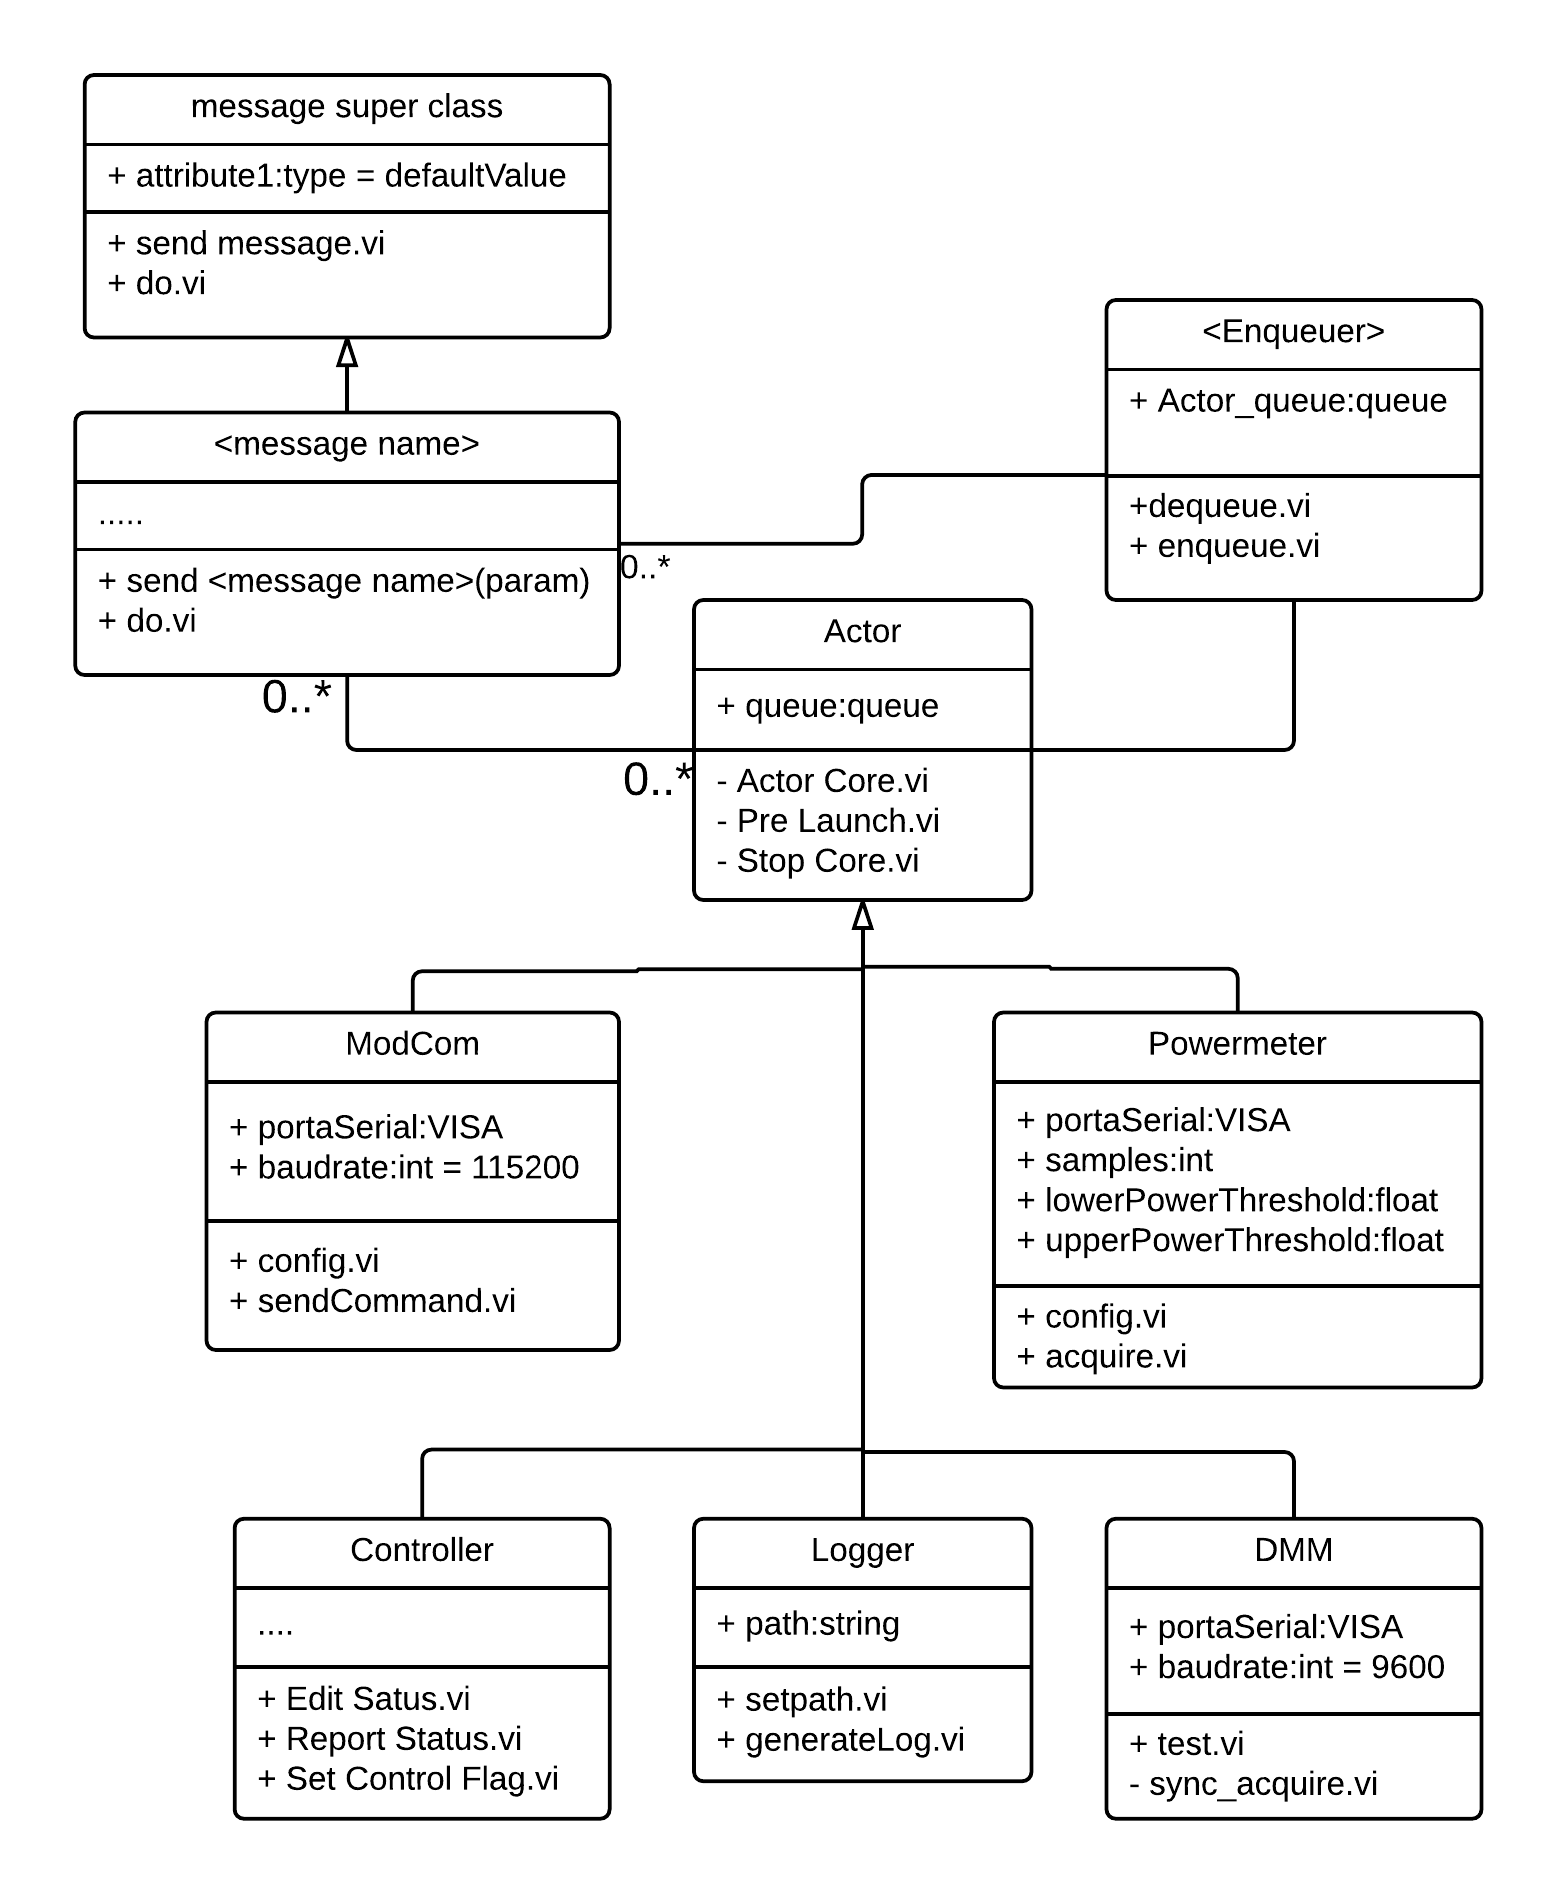
\includegraphics[width=1.4\linewidth, angle=90]{model/class}
                \caption{Diagrama de classes}
                \label{fig:classdiagram}
            \end{figure}
            
            %https://decibel.ni.com/content/docs/DOC-42227
        
        \subsection{Fluxograma da bateria de testes}
            O Fluxograma da bateria de testes é exposto na figura \ref{fig:flowchart}. Este é o fluxograma do roteiro de testes que se mantém desde antes do início deste trabalho. Nota-se que a única etapa fracionada para execução concorrente é o teste das bandejas de cartões SIM. 
            
            Por simplificação esta estrutura foi inicialmente mantida, mas trabalhos futuros serão realizados para a otimização do roteiro.
            
            \begin{figure}
                \centering
                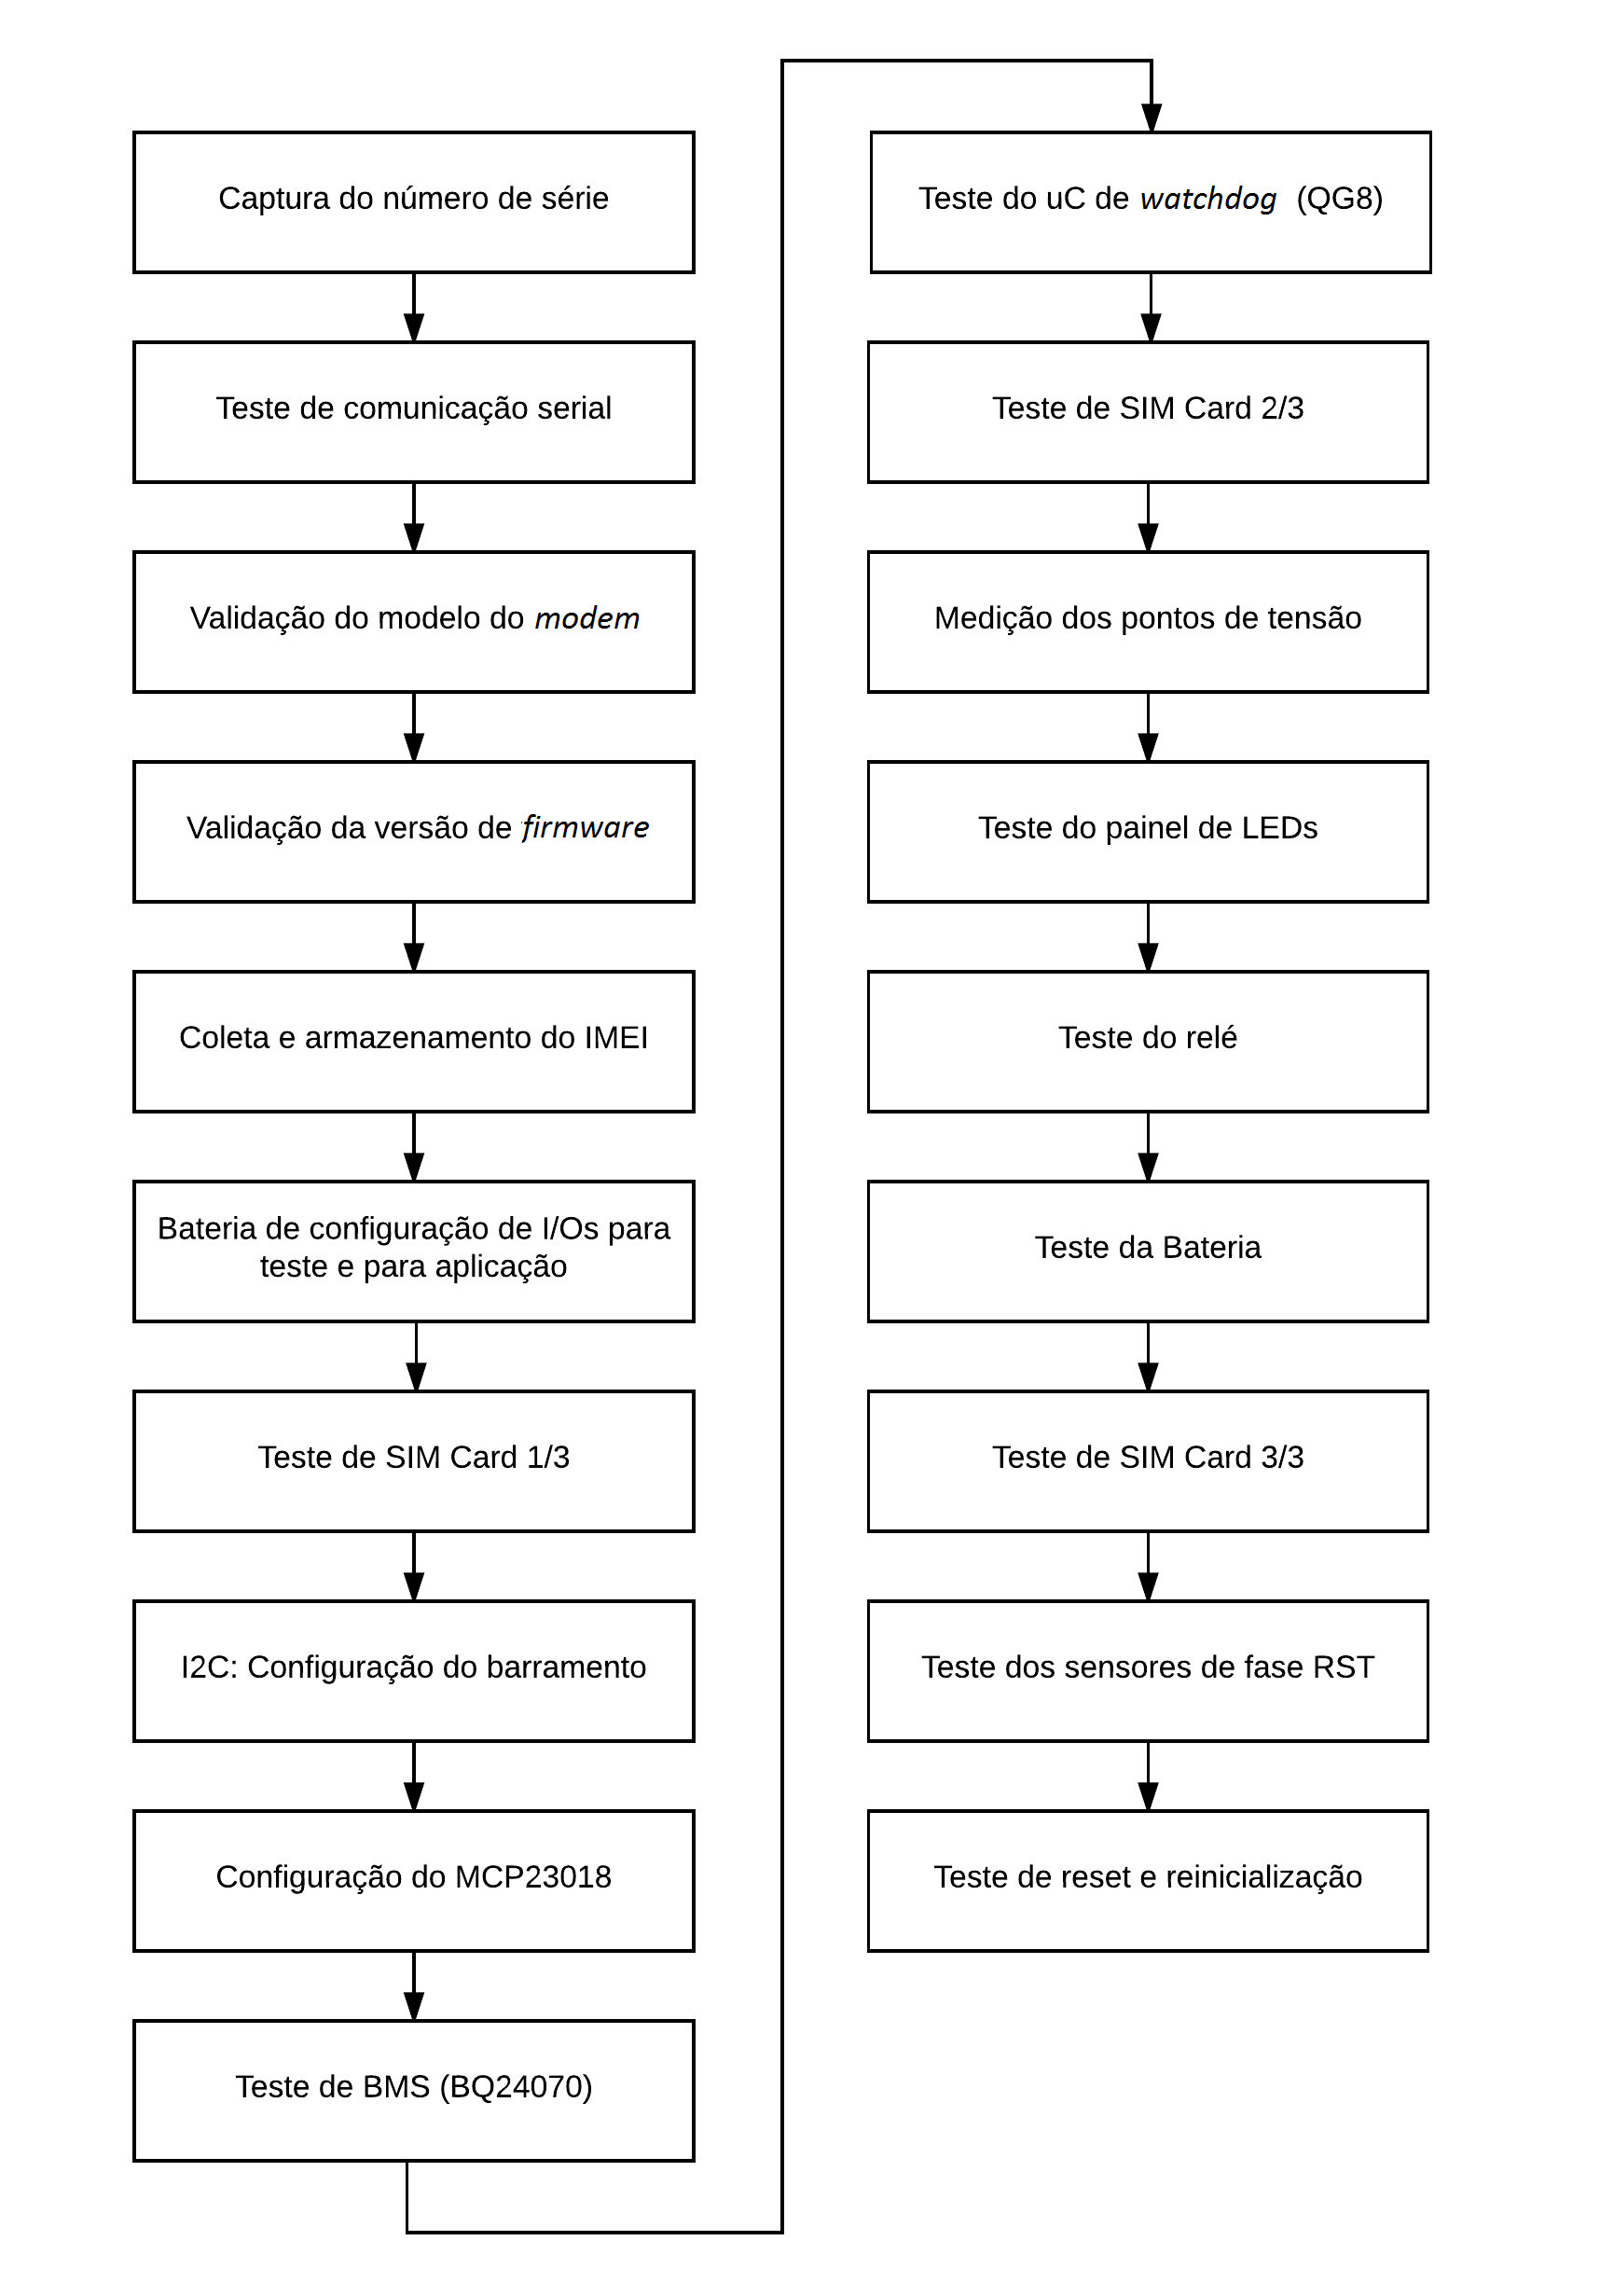
\includegraphics[width=\textwidth]{model/fluxograma}
                \caption{Fluxograma da bateria de testes}
                \label{fig:flowchart}
            \end{figure}
        
    \clearpage
    \section{Implementação}
    
        A ultima sessão foi dedicada a entender e modelar o problema a partir de uma solução proposta. Nesta sessão descreveremos a implementação dos módulos do programa de teste sob a perspectiva do modelo de atores e do framework de atores da Labview.
        
        Revendo a figura \ref{fig:modelo} vemos que o sistema em operação é composto por cinco módulos:
        \begin{itemize}
            \item Controlador;
            \item Módulo de Comunicação - \textit{Modcom};
            \item Gerador de Registros - \textit{Logger};
            \item Multímetro digital - DMM;
            \item Medidor de potência do \textit{front-end} - \textit{Powermeter}.
        \end{itemize} 
        
        Todos estes módulos possuem a implementação do \textit{framework}, através da herança da classe \textit{actor} e da classe \textit{actor message}. Todo ator tem que implementar a função \textit{actor core.vi} para poder alterar o comportamento do ator. Como o próprio nome diz, esta é a função núcleo do ator, e é responsável por inicializá-lo e executar o \textit{loop} de tratamento de mensagens. Também é possível, e recomendável, inserir nesta função, outras subrotinas, como, por exemplo, tratadores de eventos - que é um componente do controlador, que veremos a seguir.
        
        \subsection{Implementação do comunicador serial}
        
        A comunicação serial é feita por portas VISA (Virtual Instrument Software Achitecture), que são o padrão da National Instruments para configuração, programação, comunicação, e solução de problemas de sistemas de instrumentação. No ambiente Labview, comunicações seriais são abertas por meio de uma camada VISA.
        
        Na figura \ref{fig:serialcored}, pode-se ver a função básica criada para realizar toda a comunicação com o modem da placa. Sua função é enviar comandos e esperar pela resposta padrão ou esgotamento do tempo de resposta.
        
        O diagrama de blocos do ator comunicador é mais enxuto do que o controlador, pois não possui uma estrutura reativa a eventos (figura \ref{fig:modcomcore}).
        
        Após sua configuração - porta serial a ser usada, \textit{baudrate}, etc - o ator está pronto para comunicar com o módulo. Após receber do controlador o bloco de testes para ser executado, o ator executa a rotina e reporta ao Controlador os dados de resposta, assim como o diagnóstico de aprovação ou reprovação.
        
        Um exemplo interessante de um dos blocos de teste pode ser visto na figura \ref{fig:modcomledd}. Este é o bloco de teste do painel LEDs do módulo, que permite que o usuário compare o painel do módulo físico à um \textit{pop-up} que emula como o painel deveria estar (figura \ref{fig:modcomledp}). Comparada à solução anterior, que era baseada em texto e com inserção de respostas via terminal, essa foi uma alternativa mais ergonômica para o operador, reduzindo erros e aumentando a velocidade desta etapa de teste.
            
        
        \begin{figure}
                \centering
                 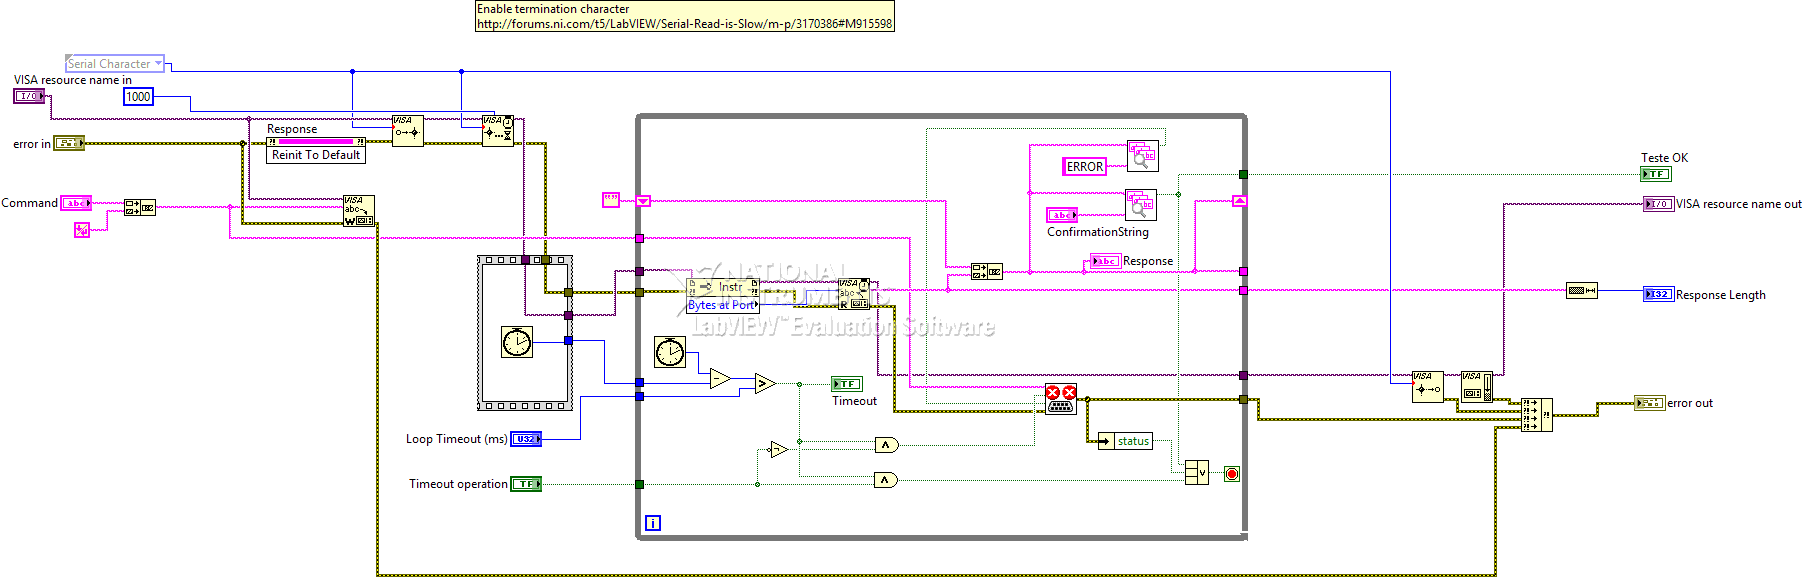
\includegraphics[width=1\linewidth]{lv/modcom/ModCOM_serialcored}
                \caption{Captura de tela da função básica de teste serial}
                \label{fig:serialcored}
        \end{figure}
        
        \begin{figure}
                \centering
                 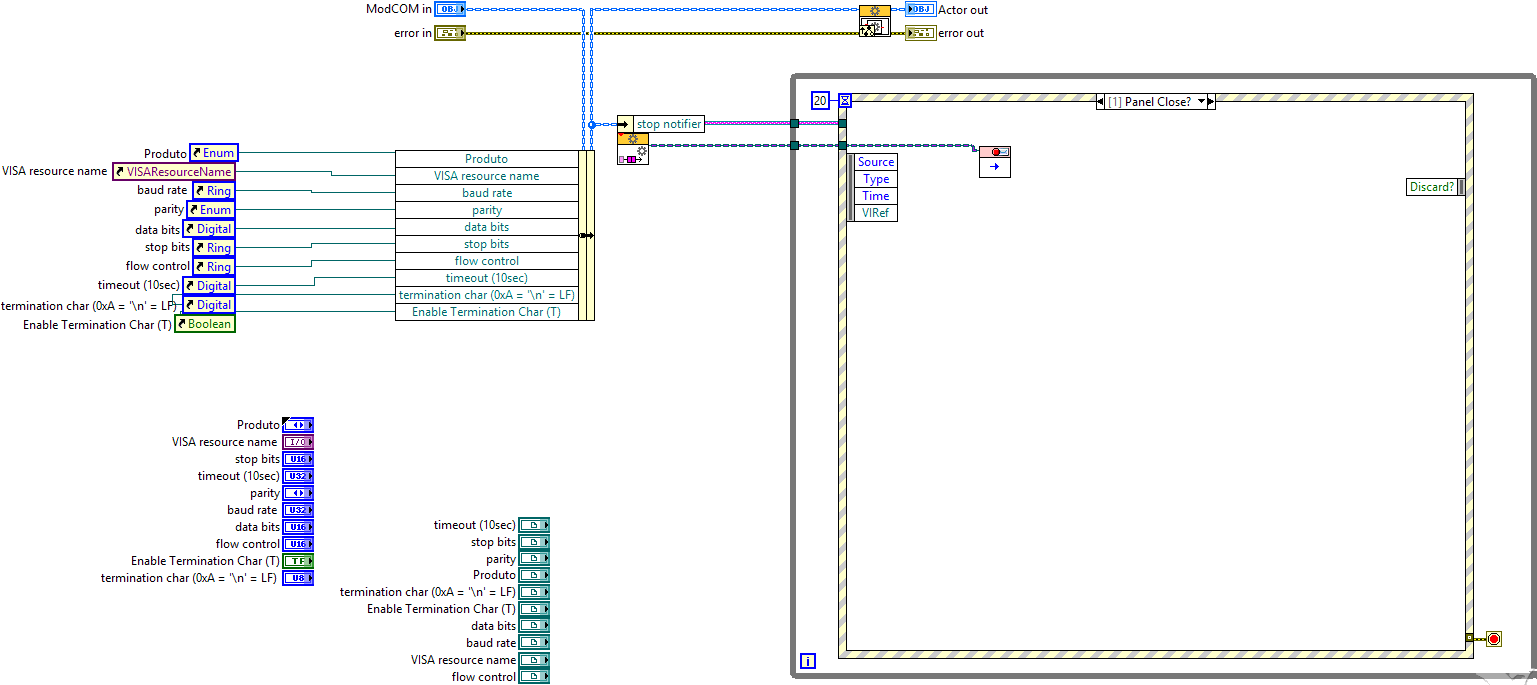
\includegraphics[width=1\linewidth]{lv/modcom/ModCOM_lvclass_Actor_Cored}
                \caption{Captura de tela do Actor Core do comunicador serial}
                \label{fig:modcomcore}
        \end{figure}
        
        \begin{figure}
                \centering
                 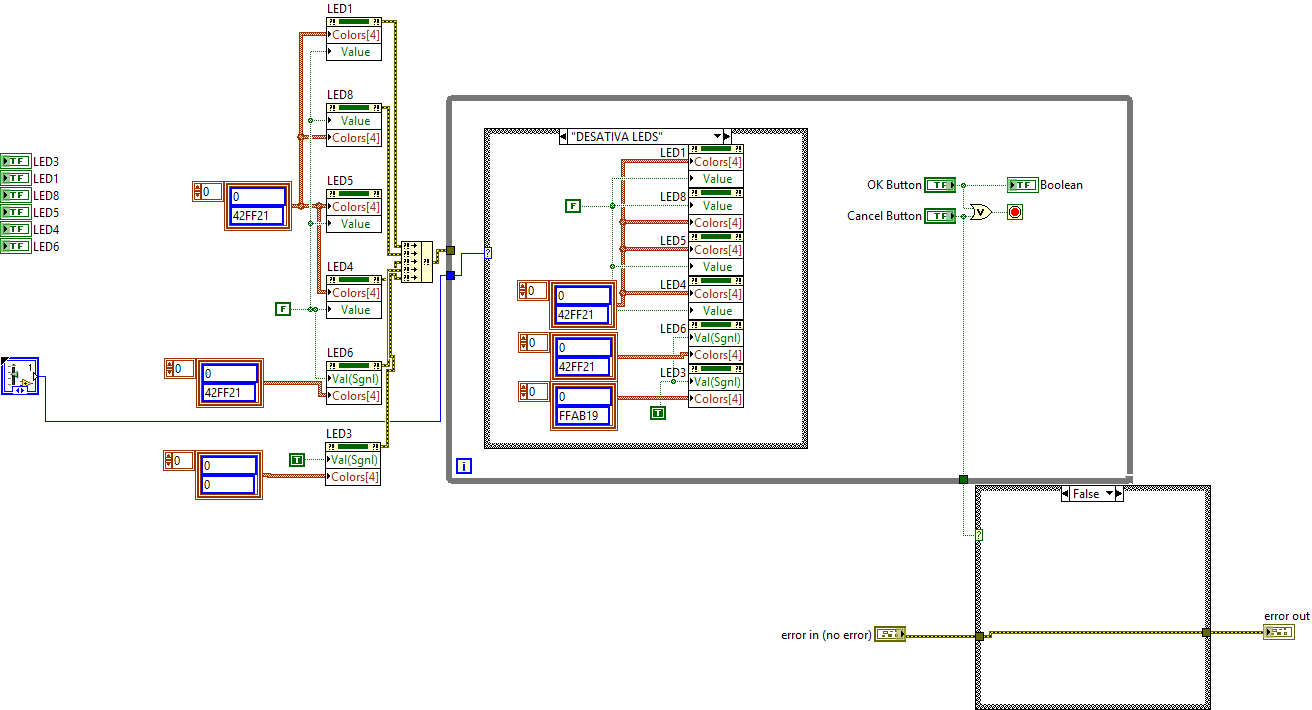
\includegraphics[width=1\linewidth]{lv/modcom/ModCOM_LED_popupd}
                \caption{Captura de tela do Diagrama de Blocos da rotina de testes de LEDs e GPIOs}
                \label{fig:modcomledd}
        \end{figure}
        
        
        
        \begin{figure}
                \centering
                 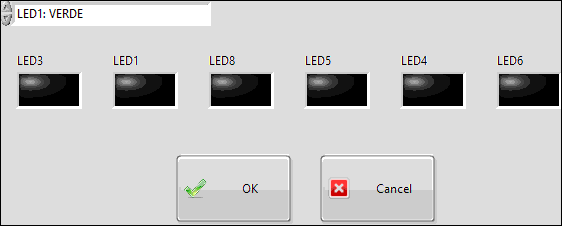
\includegraphics[width=1\linewidth]{lv/modcom/ModCOM_LED_popupp}
                \caption{Captura de tela do Painel Frontal de testes de LEDs e GPIOs}
                \label{fig:modcomledp}
        \end{figure}
        % parte oculta de diagramas
        \begin{comment}
        
         \begin{figure}
                \centering
                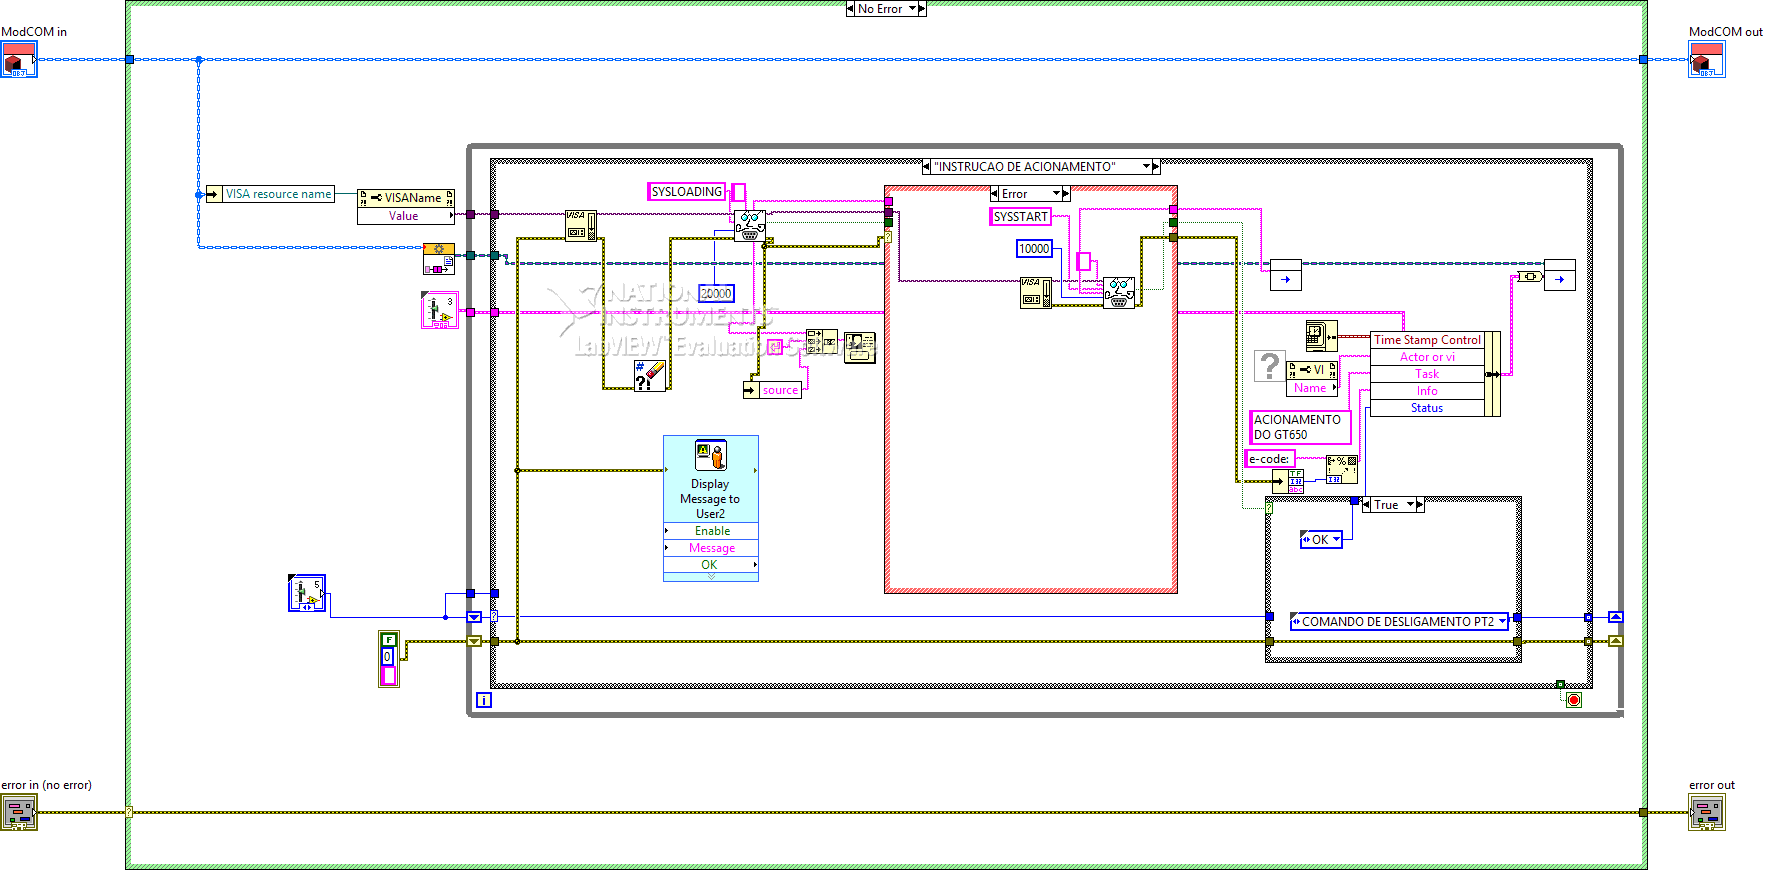
\includegraphics[width=1\linewidth]{lv/modcom/ModCOM_lvclass_desligamentoresetd}
                \caption{Captura de tela do Rotina de desligamento e reset do modem}
                \label{fig:modcomshutdown}
        \end{figure}
        
        
        \begin{figure}
                \centering
                 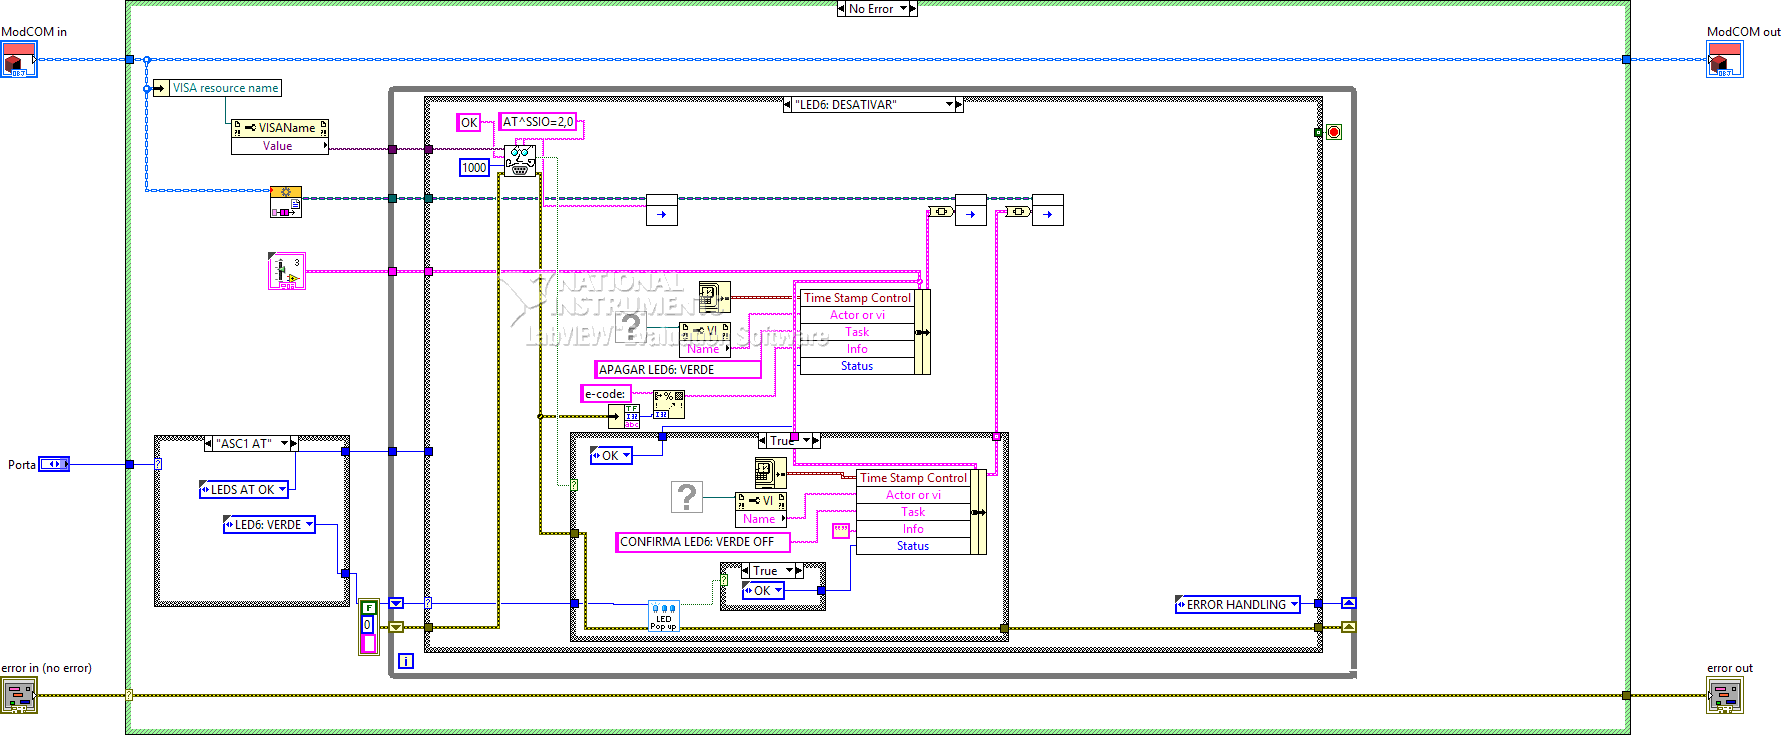
\includegraphics[width=1\linewidth]{lv/modcom/ModCOM_LED_I2Cd}
                \caption{Captura de tela do comunicador i2c}
                \label{fig:modcomledi2c}
        \end{figure}
        
        
        \begin{figure}
                \centering
                 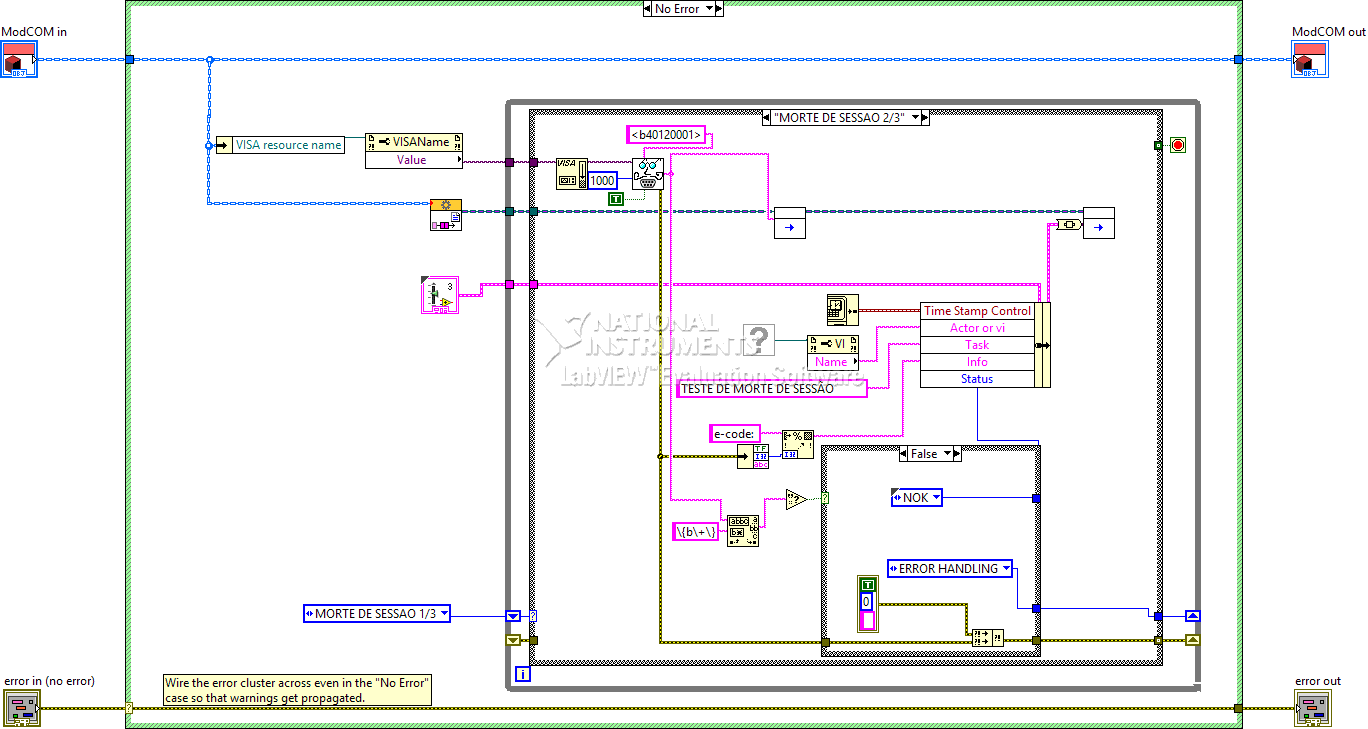
\includegraphics[width=1\linewidth]{lv/modcom/ModCOM_morted}
                \caption{Captura de tela do Teste de fechamento ou morte de comunicação serial}
                \label{fig:modcommorte}
        \end{figure}
        
        \begin{figure}
                \centering
                 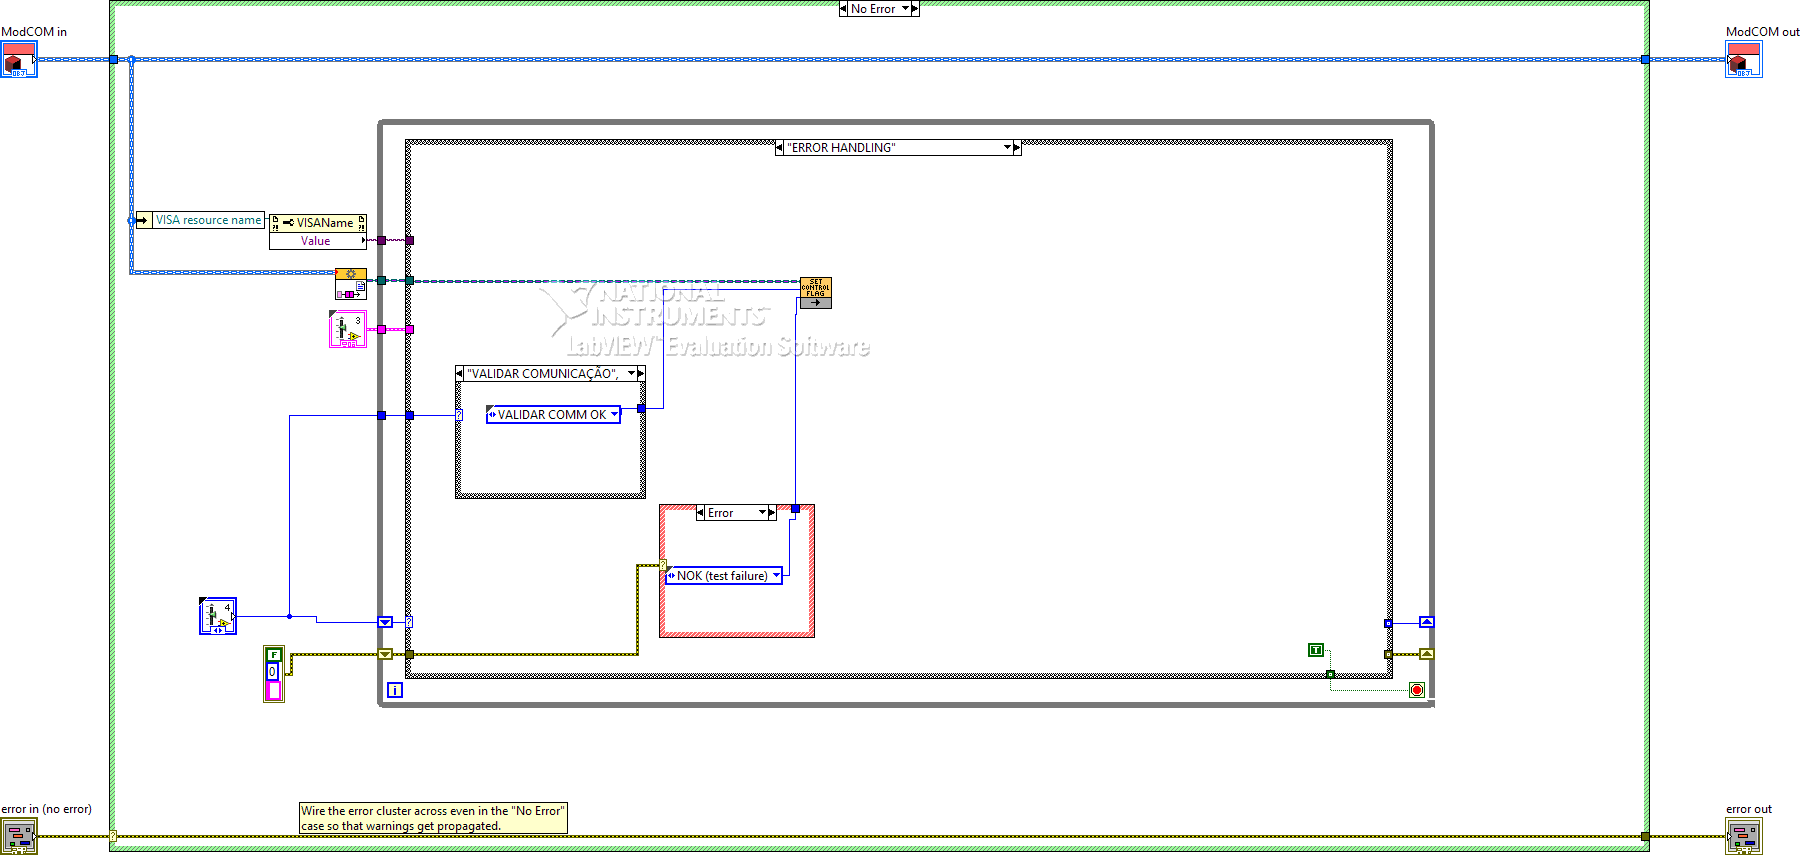
\includegraphics[width=1\linewidth]{lv/modcom/ModCOM_nopsutestd}
                \caption{Captura de tela do Captura de tela da rotina de teste sem fonte de alimentação}
                \label{fig:modcomnopsu}
        \end{figure}
        
        \begin{figure}
                \centering
                 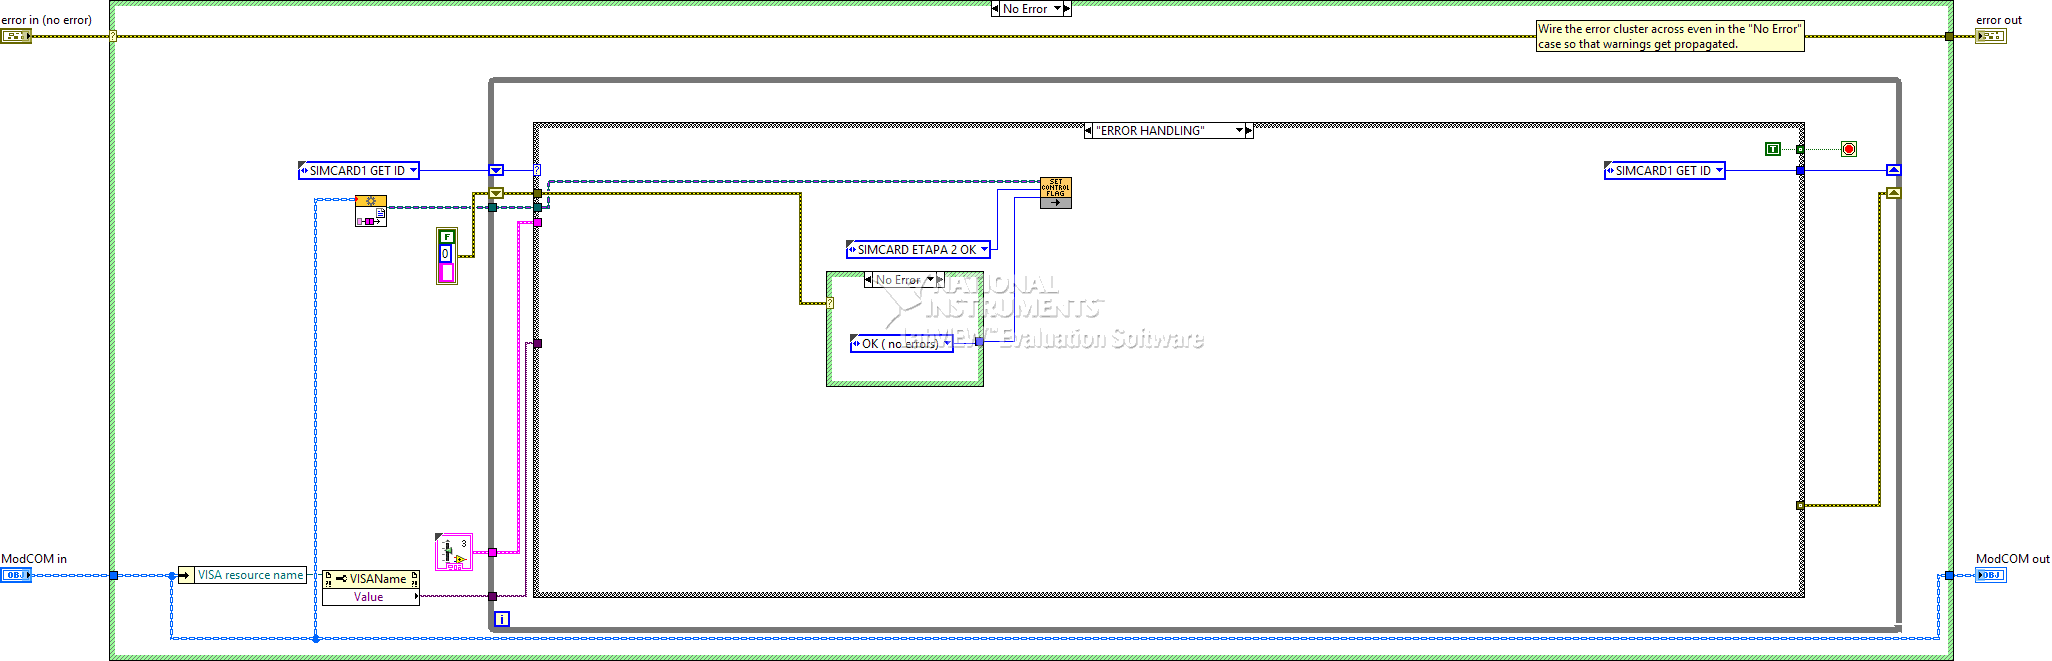
\includegraphics[width=1\linewidth]{lv/modcom/ModCOM_simcard}
                \caption{Captura de tela da rotina de teste dos simcard}
                \label{fig:modcomsimcard}
        \end{figure}
        
        \begin{figure}
                \centering
                 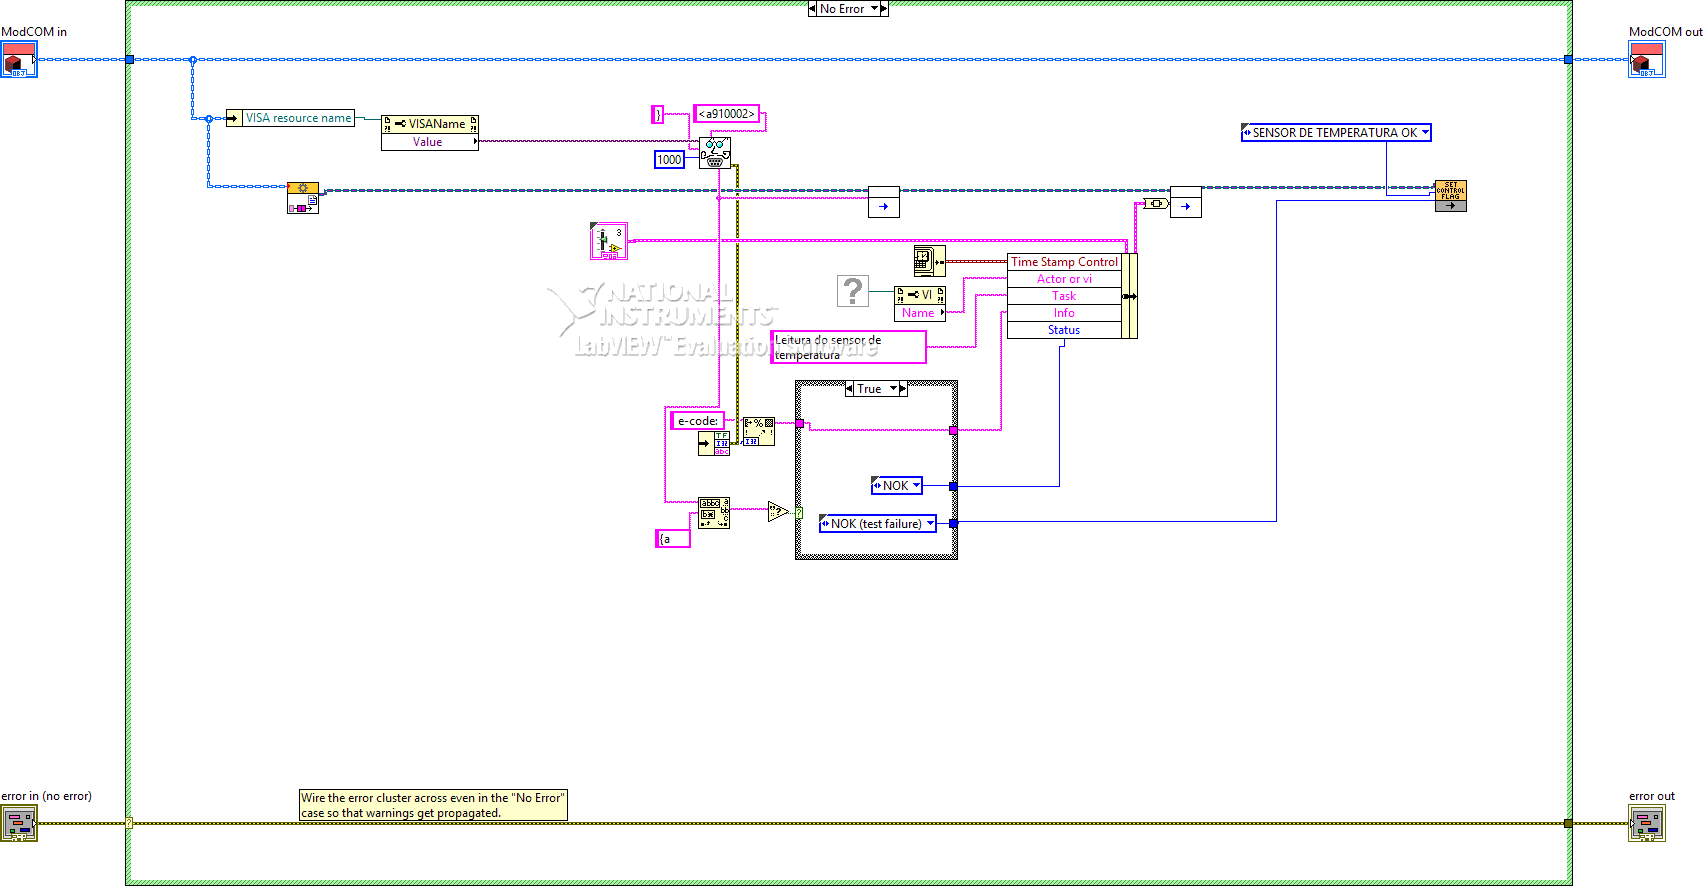
\includegraphics[width=1\linewidth]{lv/modcom/ModCOM_temp}
                \caption{Captura de tela da rotina de teste do sensor de temperatura}
                \label{fig:modcomtemp}
        \end{figure}
        
        
        \begin{figure}
                \centering
                 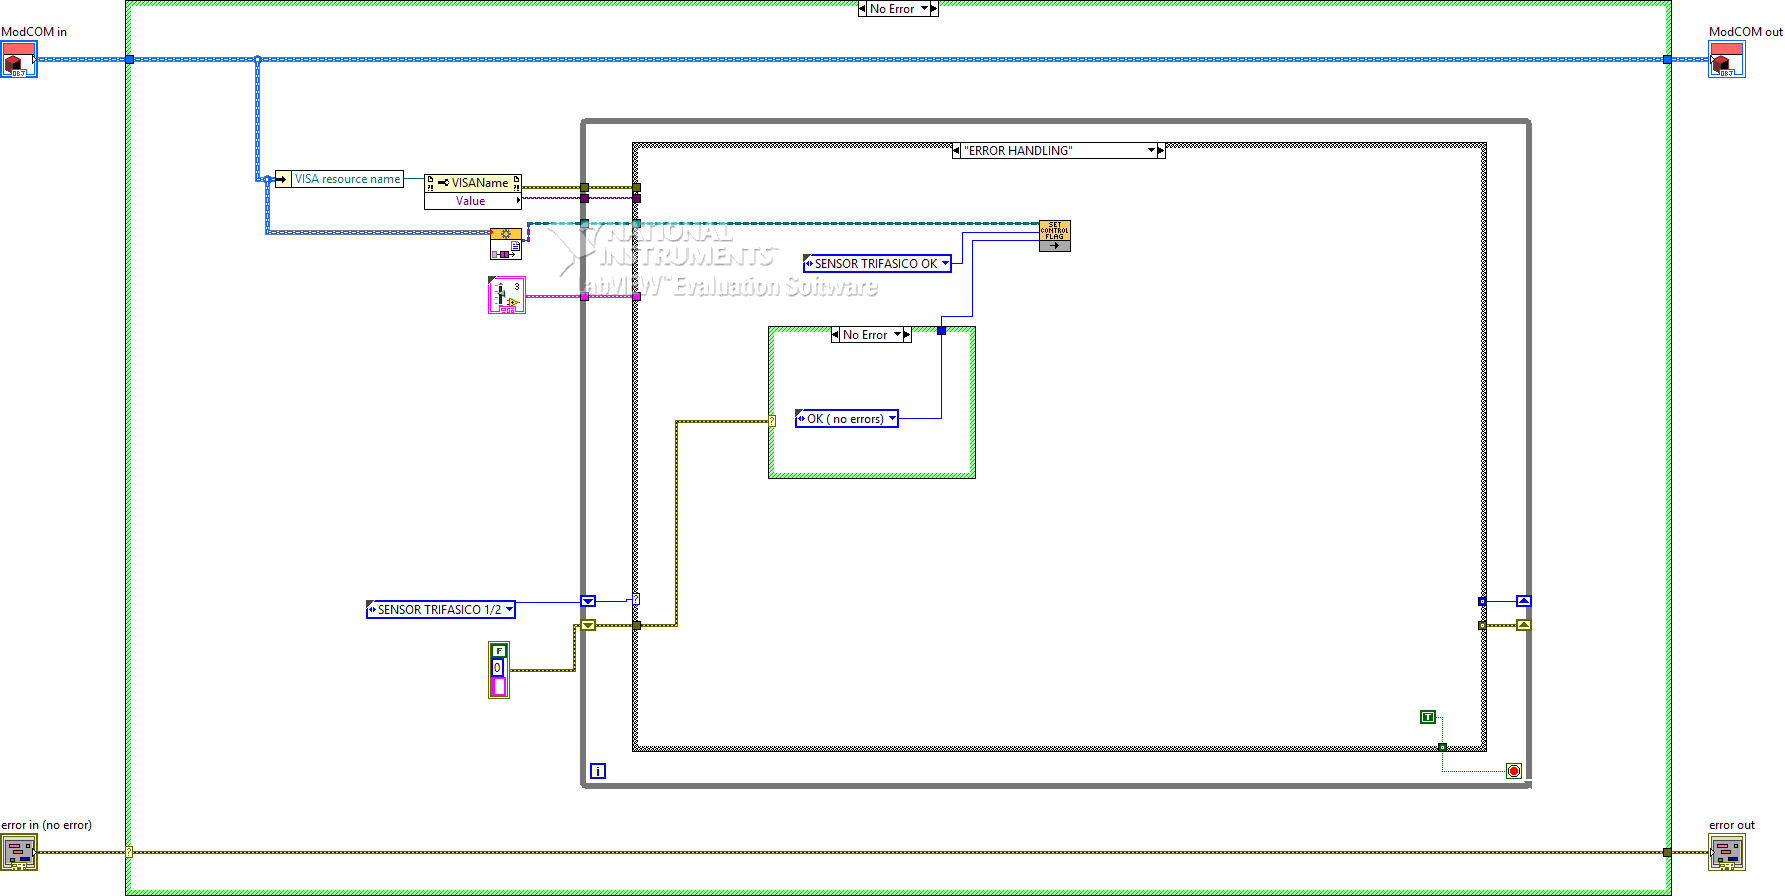
\includegraphics[width=1\linewidth]{lv/modcom/ModCOM_tritestd}
                \caption{Captura de tela da rotina de teste do sensor de presença das tensões trifásicas}
                \label{fig:modcomtri}
        \end{figure}
        
        \end{comment}
        
        \clearpage
        \subsection{Implentação do multímetro}
            % implementação Sincronização, máquina de estados 
            % figura com máquina de estados da leitura do multimetro
            %figura com os blocos e documentaçaõ da vi
            
            % vaiprecisar: diagrama de funcionamento do multimetro
            % na sessão anterior, um diagrama sobre o protocolo
            % aqui um diagrama de como lemos esse protocolo e fazemos parse
            
            Como mencionado na sessão de modelagem \ref{dmmmodel}, o ator responsável pelo multímetro precisa ler o \textit{bitstream} de leituras enviados pelo multimetro, e comparar e validar com os vetores de teste desejados.
            
            A implementação foi da seguinte forma: o \textit{bitstream} passa por uma etapa inicial de sincronização (figura \ref{fig:dmmacq}), até que se chegue ao inicio do pacote, em seguida entra em modo de aquisição, aonde o pacote é analisado e recebe significado (figuras \ref{fig:dmmbitcode} e \ref{fig:dmmparser}). Com a informação pronta, os dados vão para a interface de usuário, e junto com os vetores de pontos de teste informados pelo controlador, os valores lidos são validados em um algoritmo similar a um \textit{debouncer} (figura \ref{fig:dmmfpbd}). Explicando melhor: \textit{Se as leituras do multímetro permanecerem dentro dos limites tolerados para um determinado ponto de teste durante um período de 1 segundo, a medição é aprovada.} 
            
            Voltando à questão ergonômica, o operador não precisa tirar sua atenção da ponta de prova nos pontos de teste para ter que digitar respostas no terminal do programa. O \textit{debouncer} automaticamente passa para os próximos pontos de teste à medida que o ponto de teste é validado. E além das referencias da Interface Gráfica de Usuário (figura \ref{fig:dmmfp}), o programa emite indicações sonoras específicas em caso de aprovação, reprovação, ou nova tentativa.
            
            \begin{comment}
            \begin{figure}
                \centering
                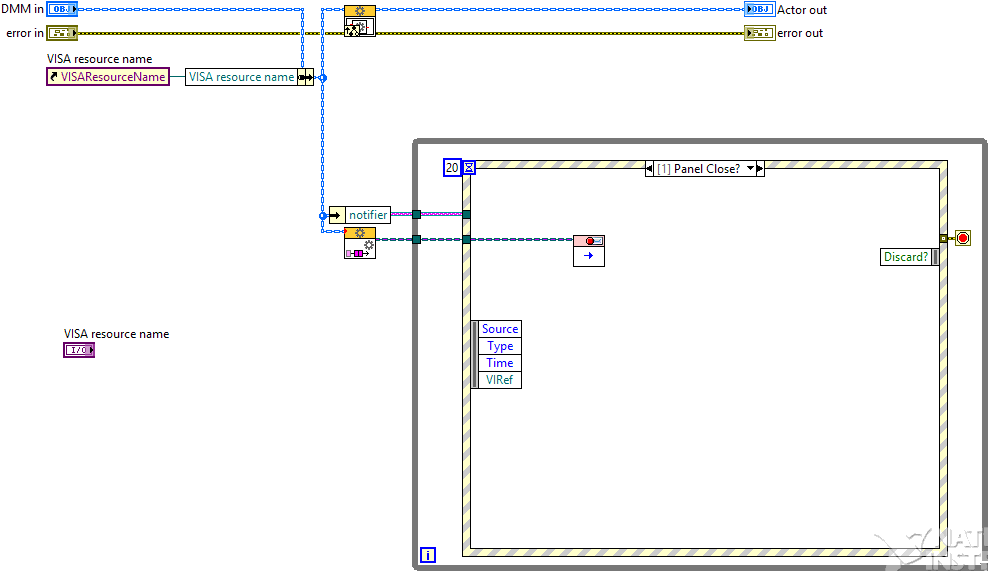
\includegraphics[width=1\linewidth]{lv/dmm/DMM_lvclass_Actor_Cored}
                \caption{Captura de tela do Actor Core do Multimetro}
                \label{fig:dmmcore}
            \end{figure}
            
            \end{comment}
            \begin{figure}
                \centering
                 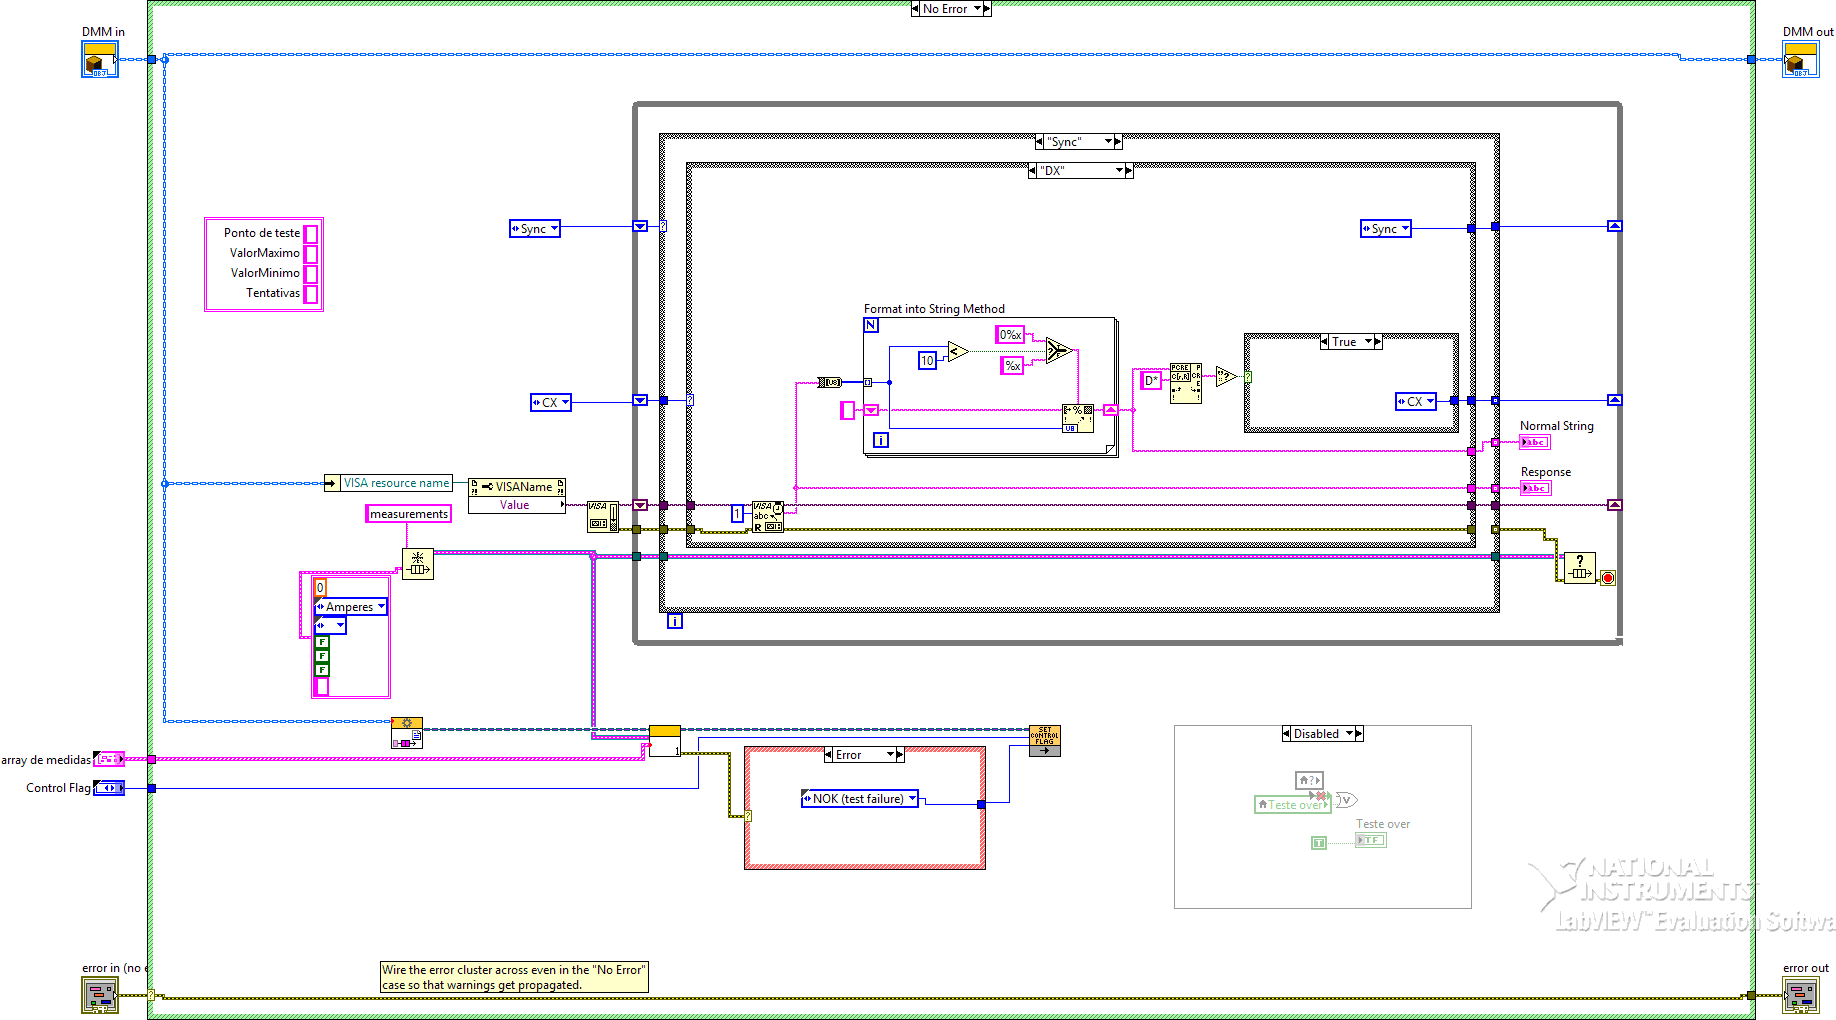
\includegraphics[width=1\linewidth]{lv/dmm/DMM_lvclass_AcquireTestpointsd}
                \caption{Captura de tela do Aquisição de dados pela serial}
                \label{fig:dmmacq}
            \end{figure}
            
            
            \begin{figure}
                \centering
                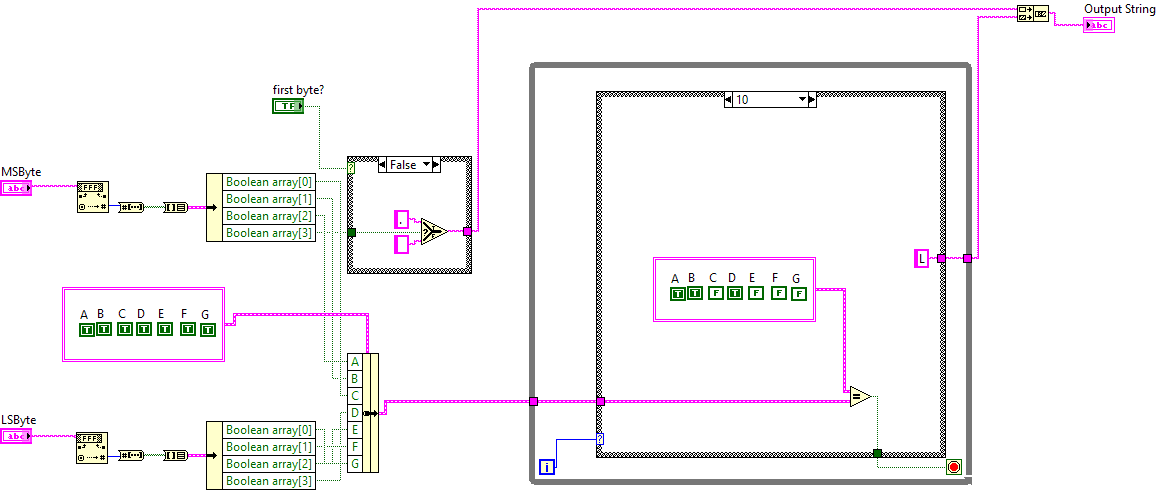
\includegraphics[width=1\linewidth]{lv/dmm/DMM_lvclass_bitcoded}
                \caption{Captura de tela do transformação de 7bitcode em string de números}
                \label{fig:dmmbitcode}
            \end{figure}
            
            
            \begin{figure}
                \centering
                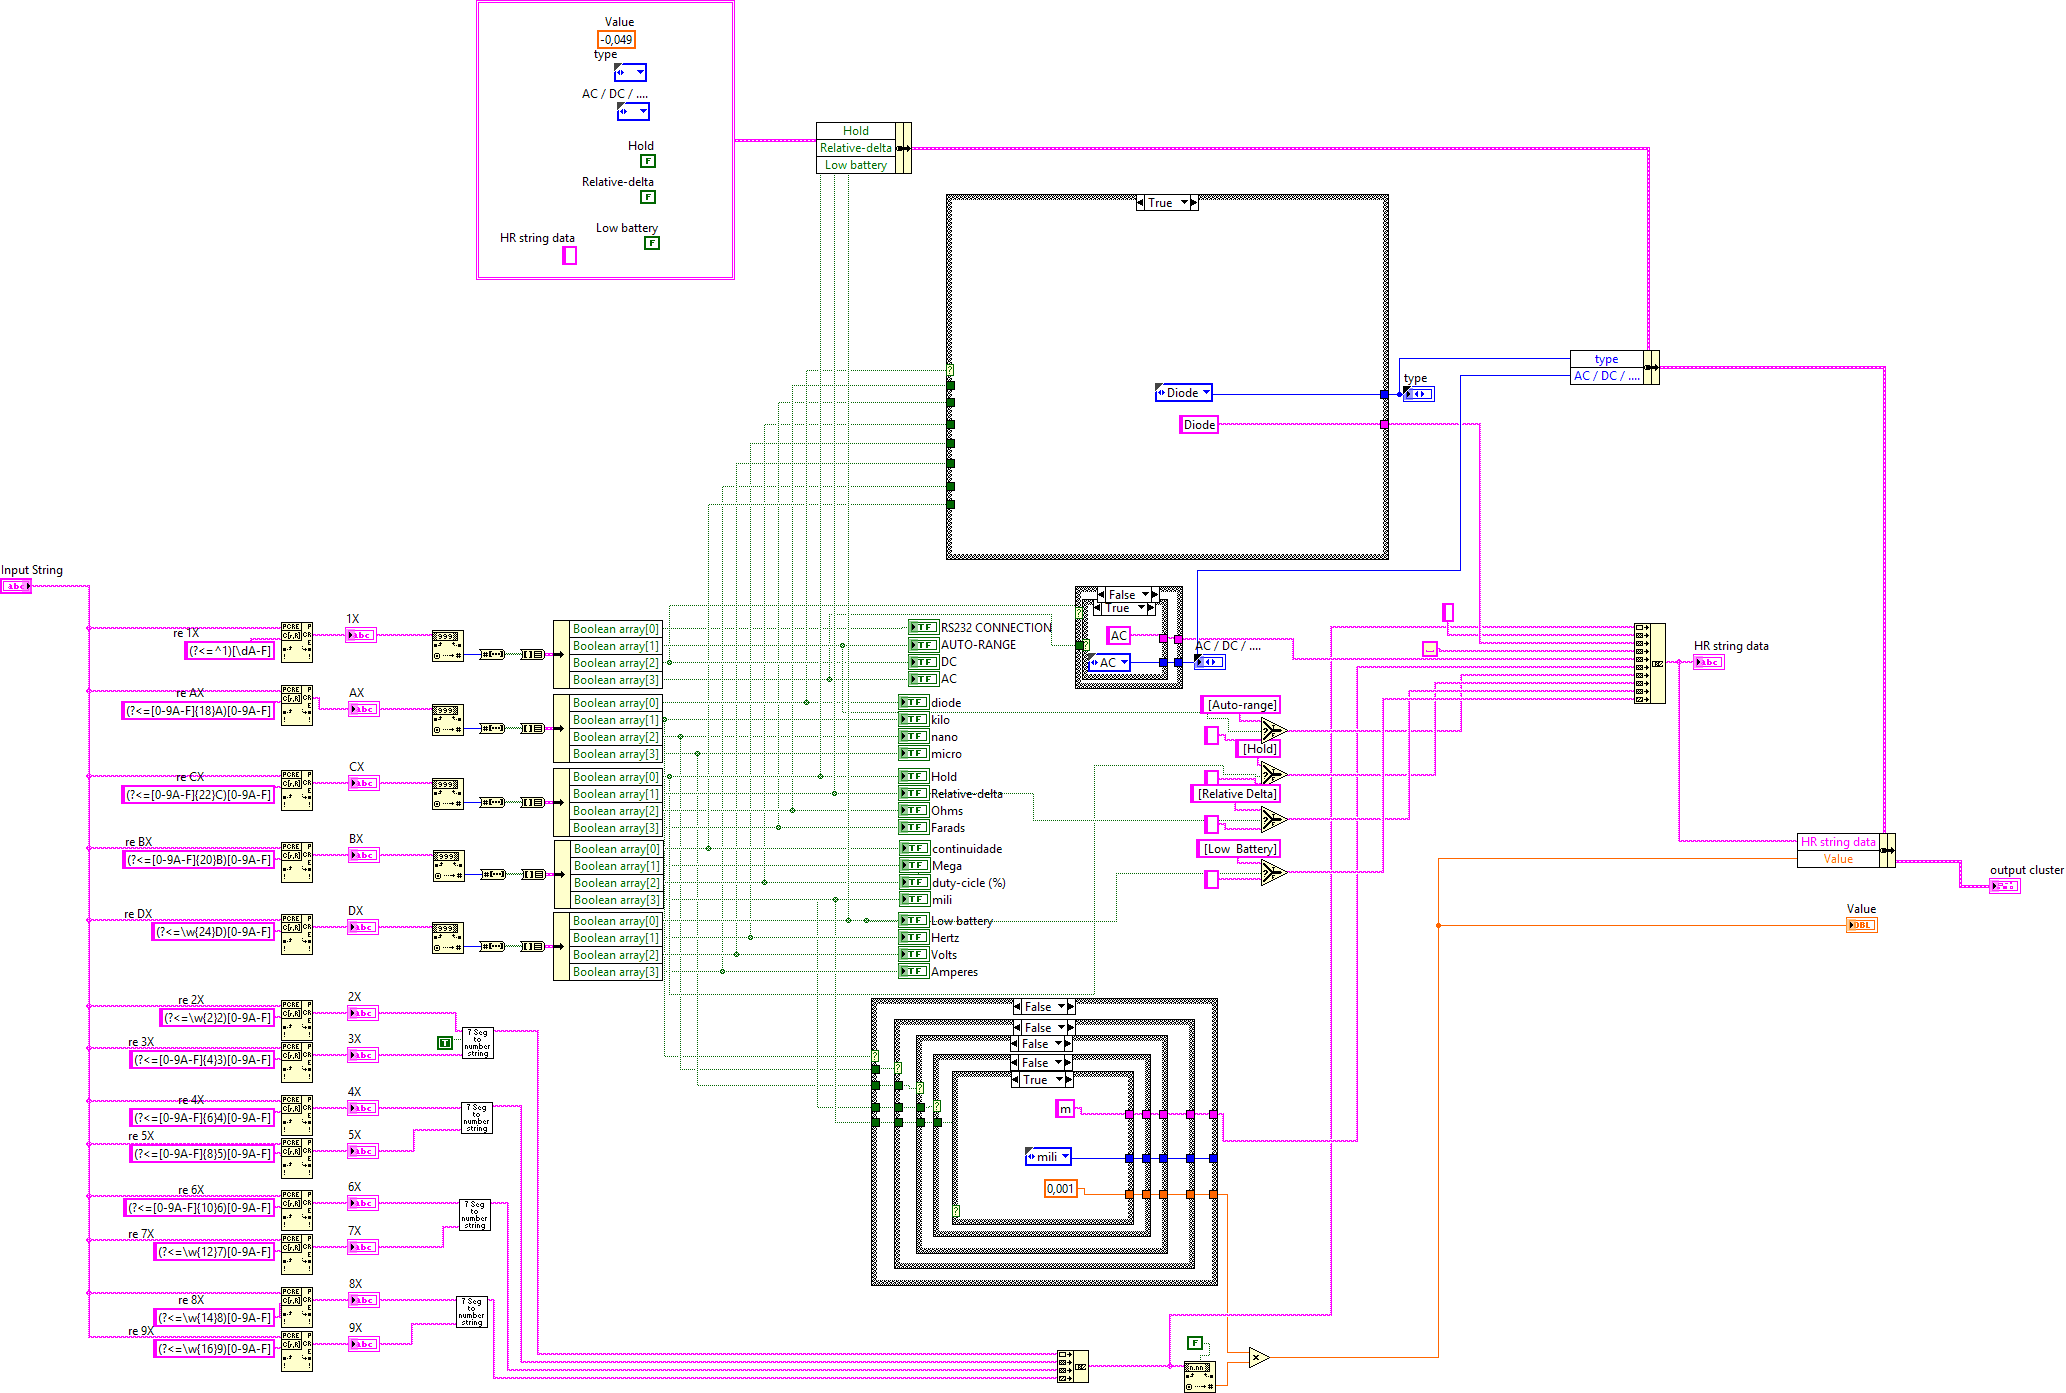
\includegraphics[width=1\linewidth]{lv/dmm/DMM_lvclass_DMM_RS232_14bit_parserd}
                \caption{Captura de tela do Parser da serial}
                \label{fig:dmmparser}
            \end{figure}
            
            
            \begin{figure}
                \centering
                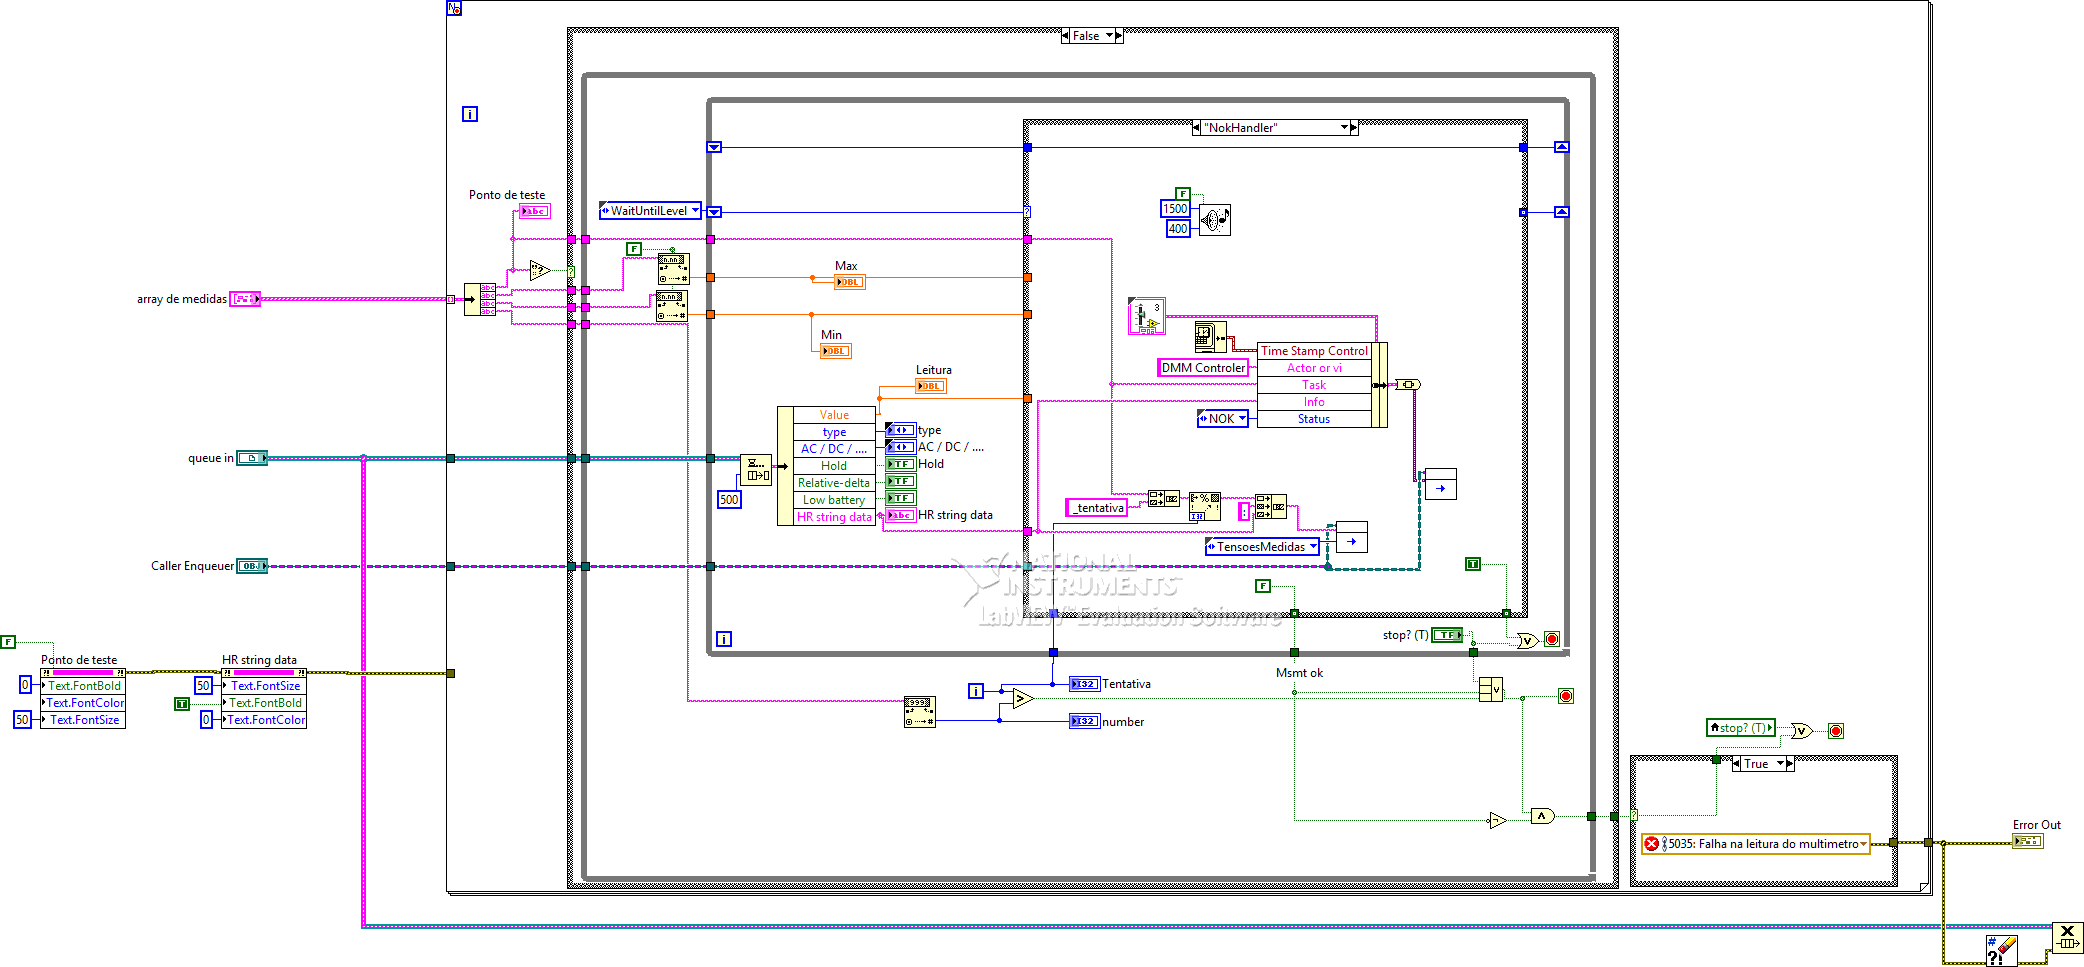
\includegraphics[width=1\linewidth]{lv/dmm/DMM_lvclass_DMM_UI_d}
                \caption{Captura de tela do Diagrama de blocos da interface de usuário}
                \label{fig:dmmfpbd}
            \end{figure}
            
            \begin{figure}
                \centering
                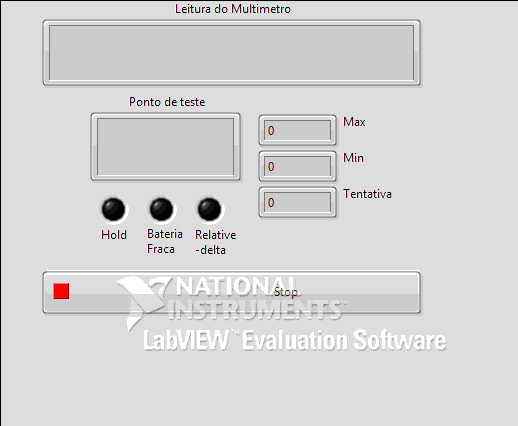
\includegraphics[width=1\linewidth]{lv/dmm/DMM_lvclass_DMM_UI_p}
                \caption{Captura de tela do Painel frontal da interface de usuário}
                \label{fig:dmmfp}
            \end{figure}
            
            
        \clearpage
        \subsection{Implentação do gerador de registros}
            
            O gerenciador de registros neste programa basicamente recebe todos os dados da execução das baterias de teste e aglutina em um documento, possibilitando a geração de arquivos de texto como também a de arquivos JSON.
            
            Mesmo que o ator suporte o envio dos arquivos para um servidor, o armazenamento dos arquivos é feito em pastas locais, já que o \textit{webservice} de registros ainda não foi adaptado para este programa.
            
            A saída padrão deste ator é composta por duas classes de registros: 
            
            Um registro com todos os dados de execução, despejo dos dados da serial, \textit{timestamps}, e com os registros de exceções de execução. Dados necessários para a depuração de problemas na placa, e para melhor efetividade no retrabalho.
            O segundo registro consiste em um resumo da bateria de testes, diagnóstico geral da placa, e qualquer informação que for valiosa para análise em massa, requisito necessário para otimizações do processo produtivo como também do próprio produto.
            
            Nas figuras \ref{fig:loggen} e \ref{fig:logmake} vemos os diagramas de blocos dos instrumentos virtuais internos desta classe, responsáveis para criação dos arquivos de registro de execução.
            
            \begin{comment}
                \begin{figure}
                    \centering
                    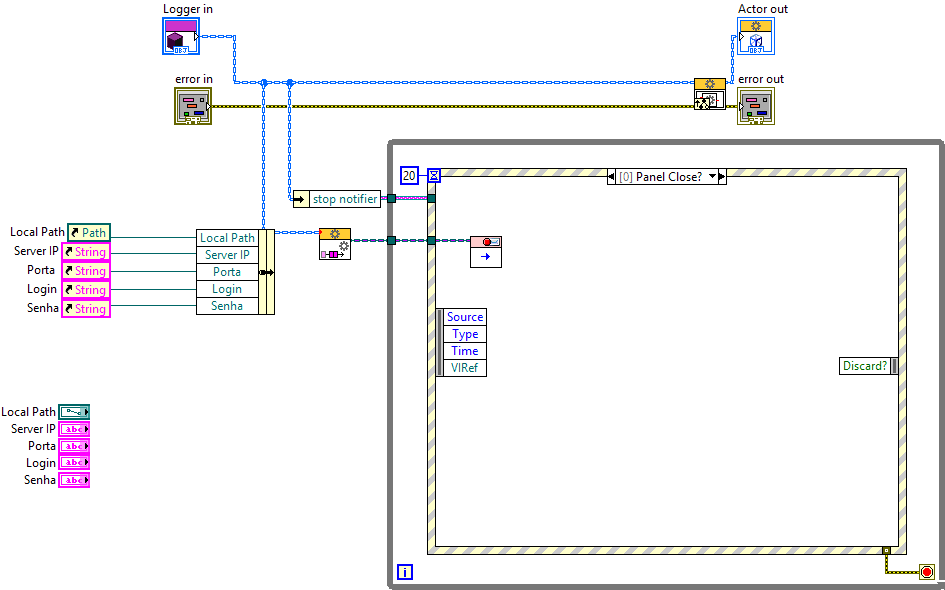
\includegraphics[width=1\linewidth]{lv/log/Logger_lvclass_Actor_Cored}
                    \caption{Captura de tela do Actor Core do Gerador de Log}
                    \label{fig:logcore}
                \end{figure}
                \begin{figure}
                    \centering
                    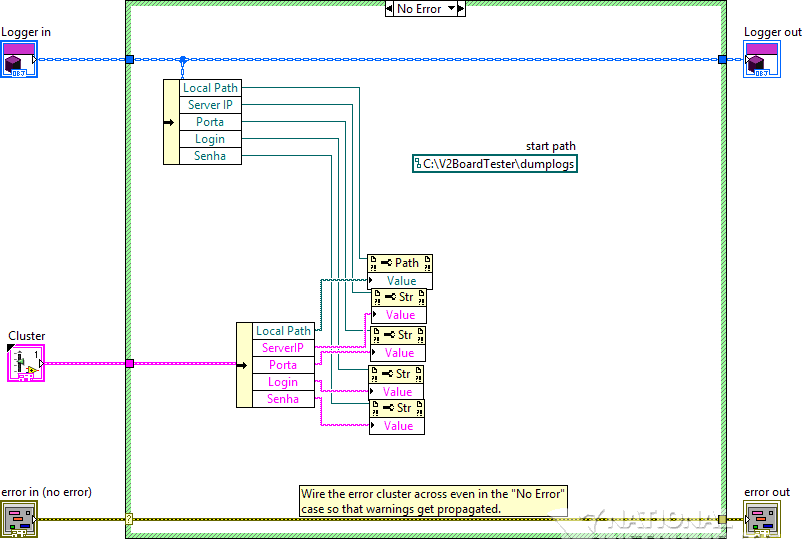
\includegraphics[width=1\linewidth]{lv/log/Logger_lvclass_Configd}
                    \caption{Captura de tela do Configurador Gerador de Log}
                    \label{fig:logconf}
                \end{figure}
            \end{comment}
            
            
            \begin{figure}
                \centering
                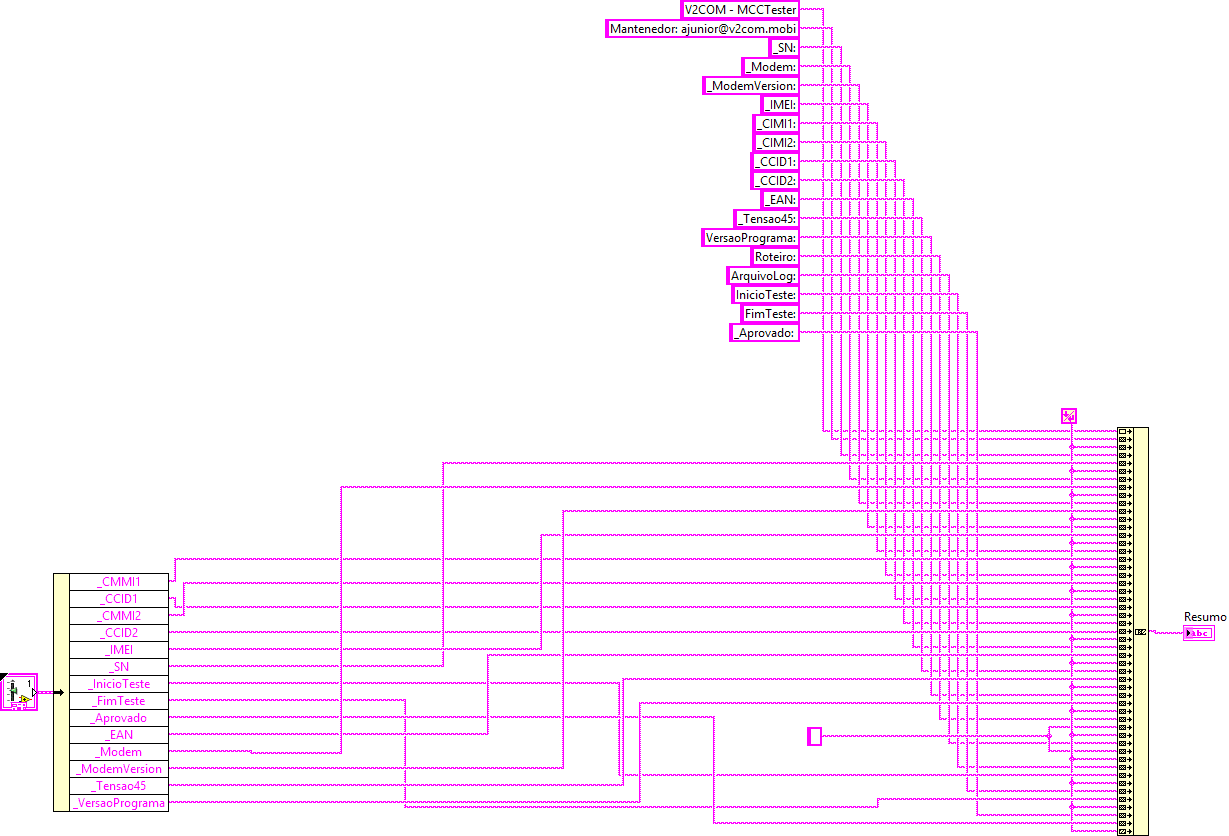
\includegraphics[width=1\linewidth]{lv/log/Logger_lvclass_LogGen_(SubVI)d}
                \caption{Captura de tela do Instrumento virtual de geraçao de log}
                \label{fig:loggen}
            \end{figure}
            \begin{figure}
                \centering
                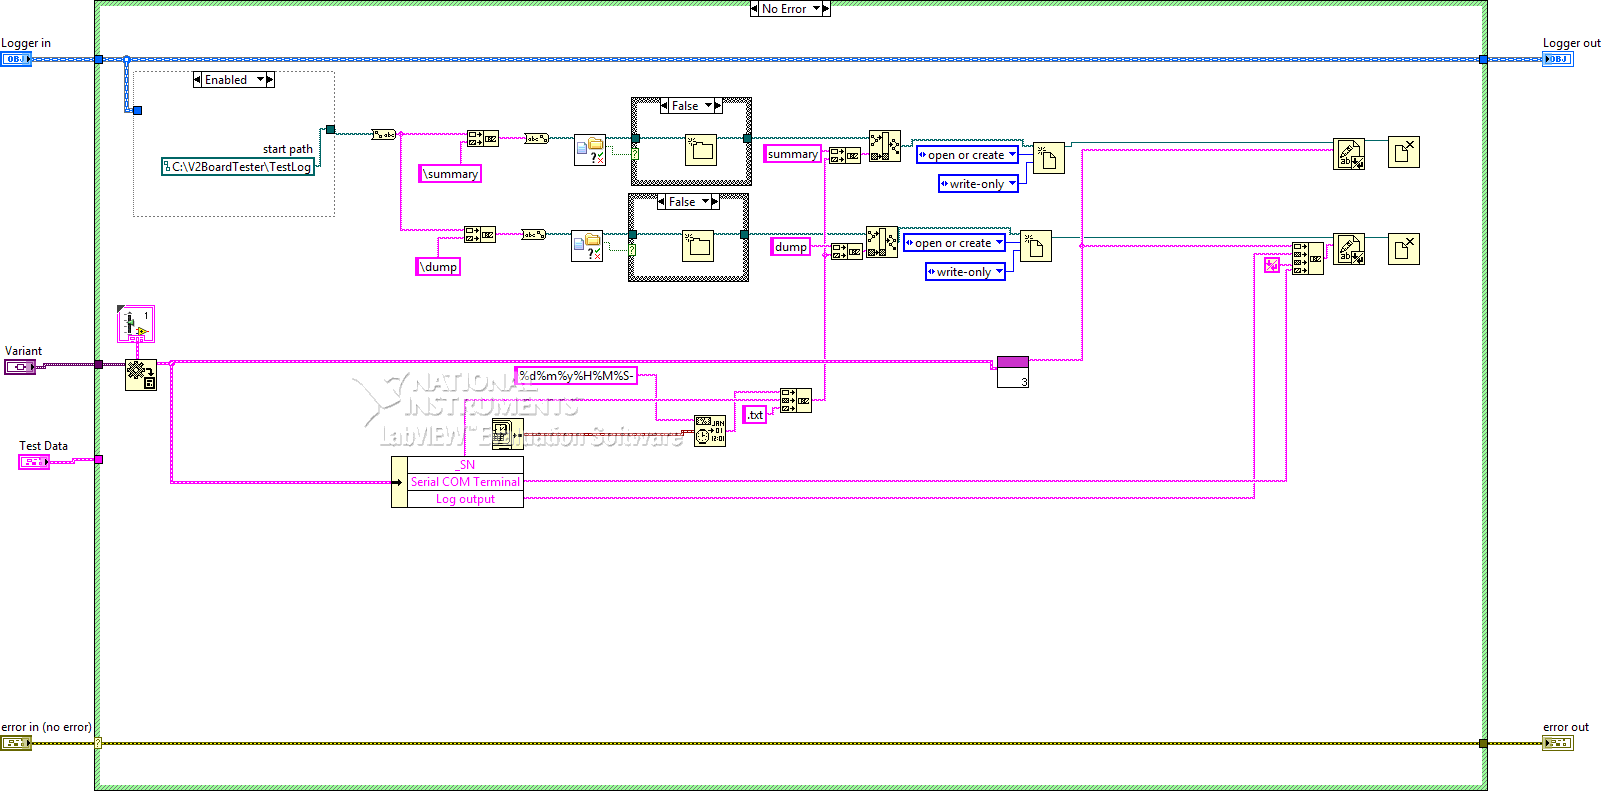
\includegraphics[width=1\linewidth]{lv/log/Logger_lvclass_MakeLogd}
                \caption{Captura de tela do Criador  de Log}
                \label{fig:logmake}
            \end{figure}
            \clearpage   
        \subsection{Implentação do medidor de potência}
            
            Como explicado na sessão \ref{pwmodel}, a implementação do medidor de potência de sinal do \textit{front-end} foi feita parcialmente, já que é realizada por outro programa e em outra etapa do processo produtivo.
            
            Apesar de fora deste escopo de trabalho, ressalta-se que foram realizados melhorias e otimizações no processo de medição de potência de front-end também.
            
            As figuras \ref{fig:pwcore} e \ref{fig:pwconf} exibem o diagrama de blocos dos instrumentos virtuais do Actor Core e de configuração do ator, respectivamente. A implementação de outros módulos dependem do interesse da empresa de realizar este teste nas empresas que prestam os serviços de montagem.
            
            \begin{figure}
                \centering
                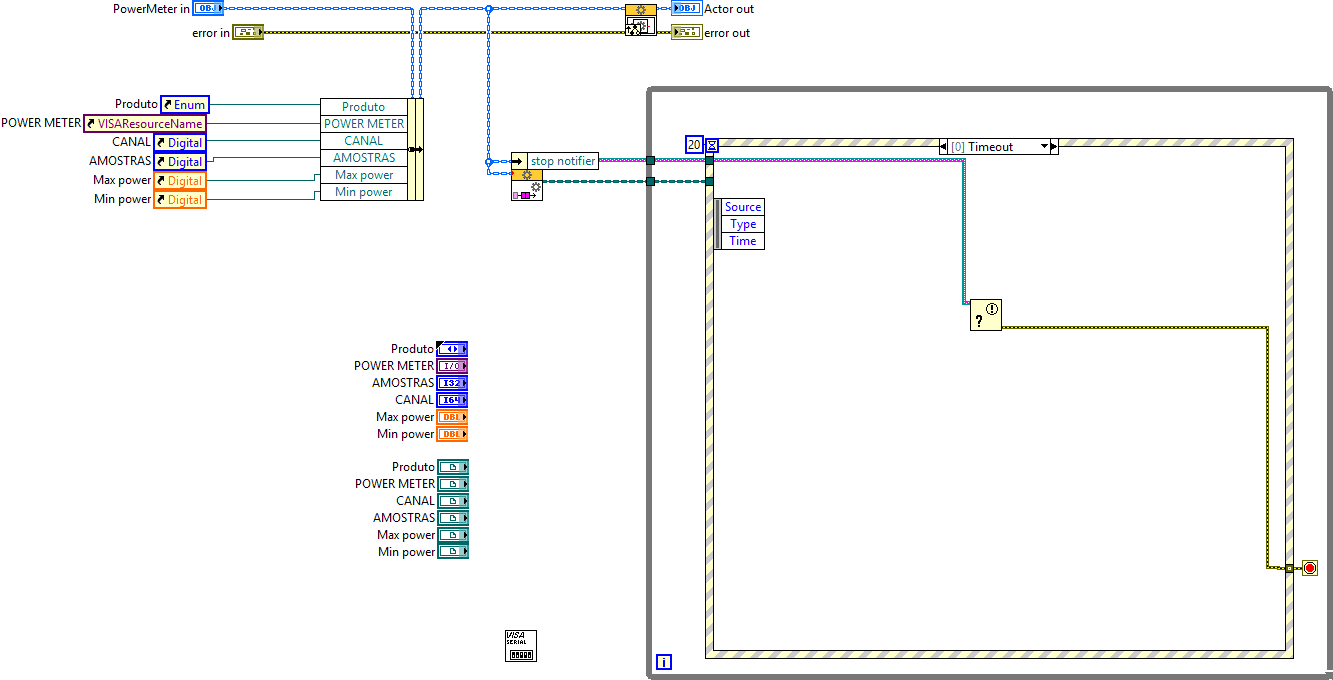
\includegraphics[width=1\linewidth]{lv/pwmtr/PowerMeter_lvclass_Actor_Cored}
                \caption{Captura de tela do Actor Core do Power Meter}
                \label{fig:pwcore}
            \end{figure}
            \begin{figure}
                \centering
                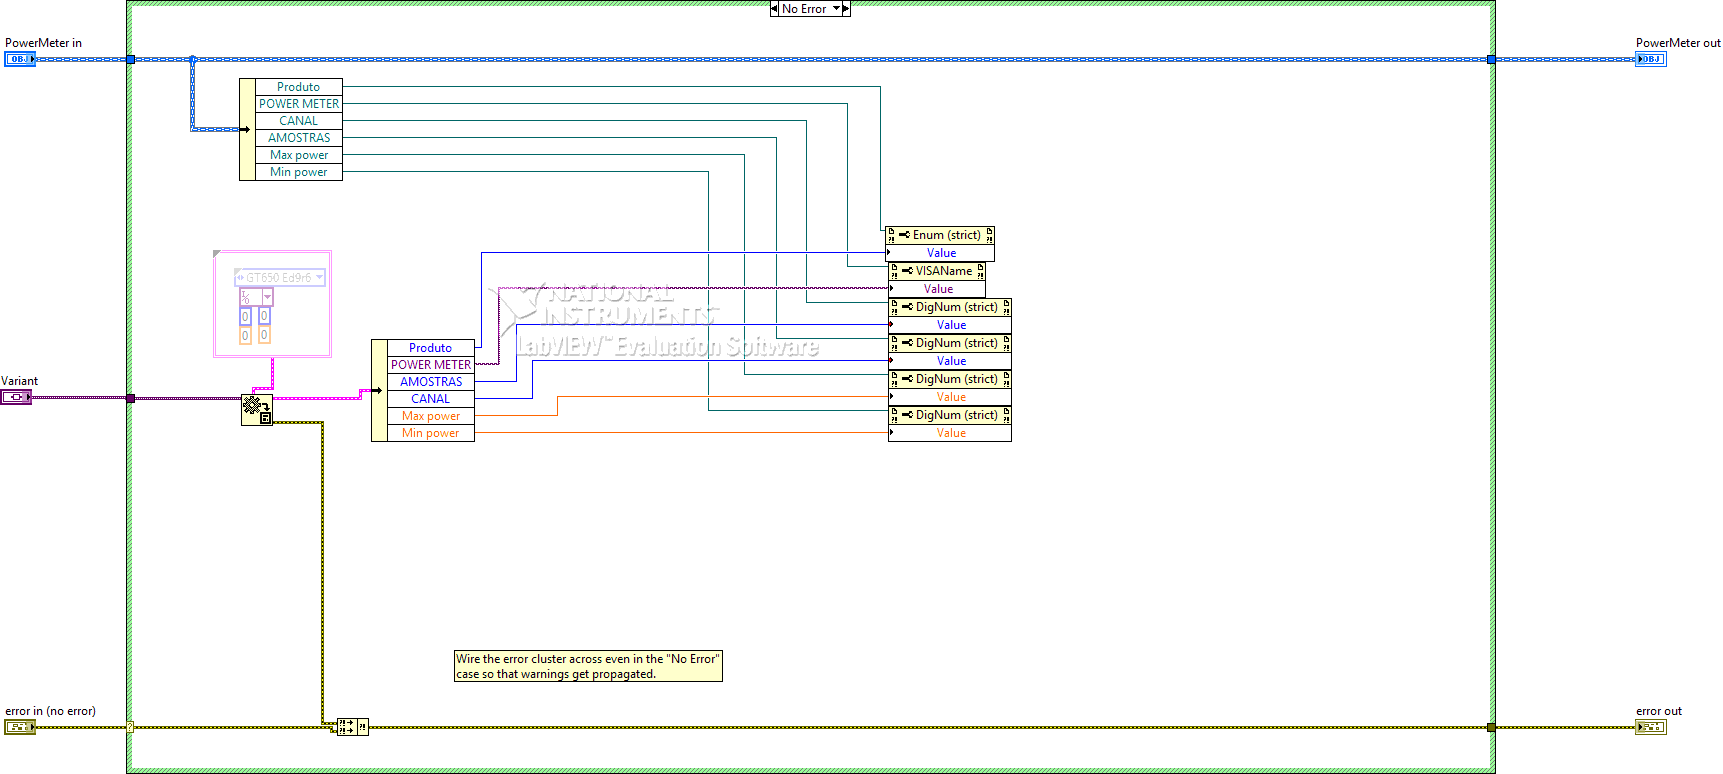
\includegraphics[width=1\linewidth]{lv/pwmtr/PowerMeter_lvclass_SET_PM_Actor_Configd}
                \caption{Captura de tela do Configuração do Power Meter}
                \label{fig:pwconf}
            \end{figure}
        \clearpage
        \subsection{Implentação do controlador}
        
        O actor core, como qualquer outro módulo do programa (figura \ref{fig:cntrlcore}). Por centralizar e fazer o controle de fluxo de teste, através de mensagens de execução e respostas sobre o status de execução, o controlador foi implementado com uma estrutura orientada à eventos. Dessa maneira, sempre que ele receber resposta de um ator filho, ele pode disparar outras mensagens de execução.
        
        Conforme já mencionado, um ator só entende mensagens que invocam métodos internos dele. Com isso em mente, foi criado um método especifico para relatar sucesso/falha de execução de subrotinas dos atores filhos ao controlador. Esta mensagem, enviada pelos atores-filhos, invoca o método interno do controlador, \textit{report control flag.vi} (figura \ref{fig:cntrlset}), o qual dispara outros eventos mencionados no parágrafo anterior.
        
        \begin{figure}
                \centering
                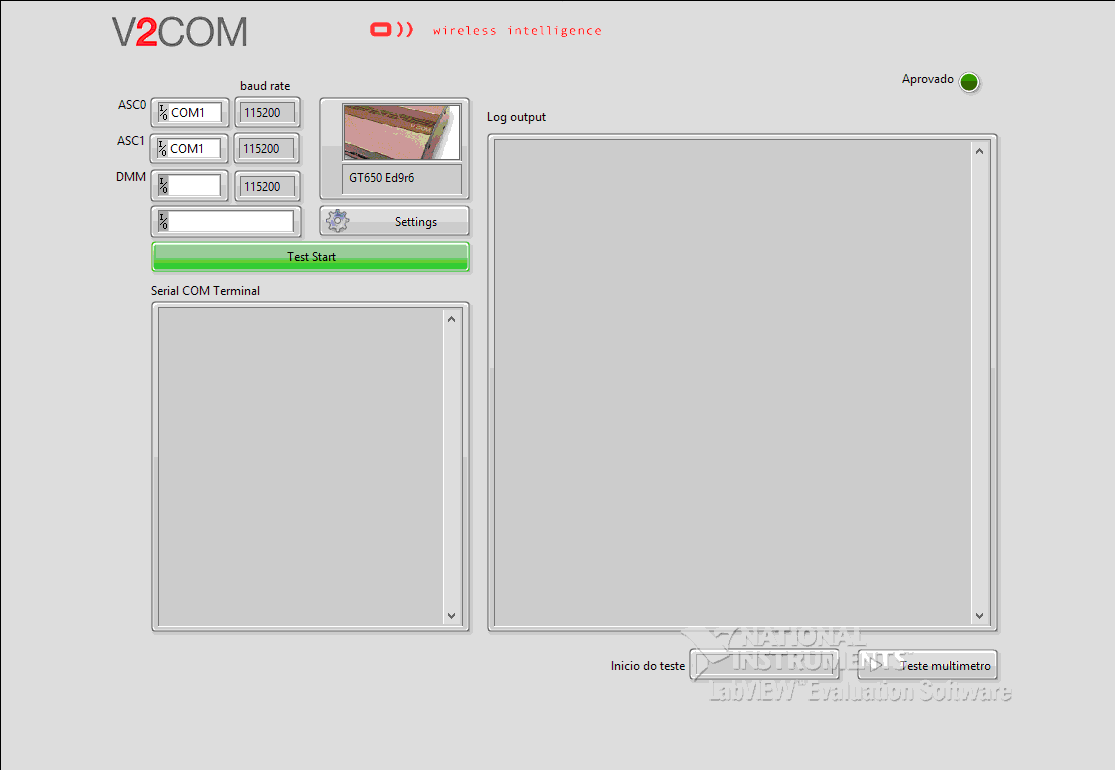
\includegraphics[width=0.8\linewidth]{lv/controler/Controller_lvclass_Actor_Corep}
                \caption{Captura de tela do Painel Frontal para a interface de usuário}
                \label{fig:cntrlpanel}
        \end{figure}
        
        \begin{figure}
                \centering
                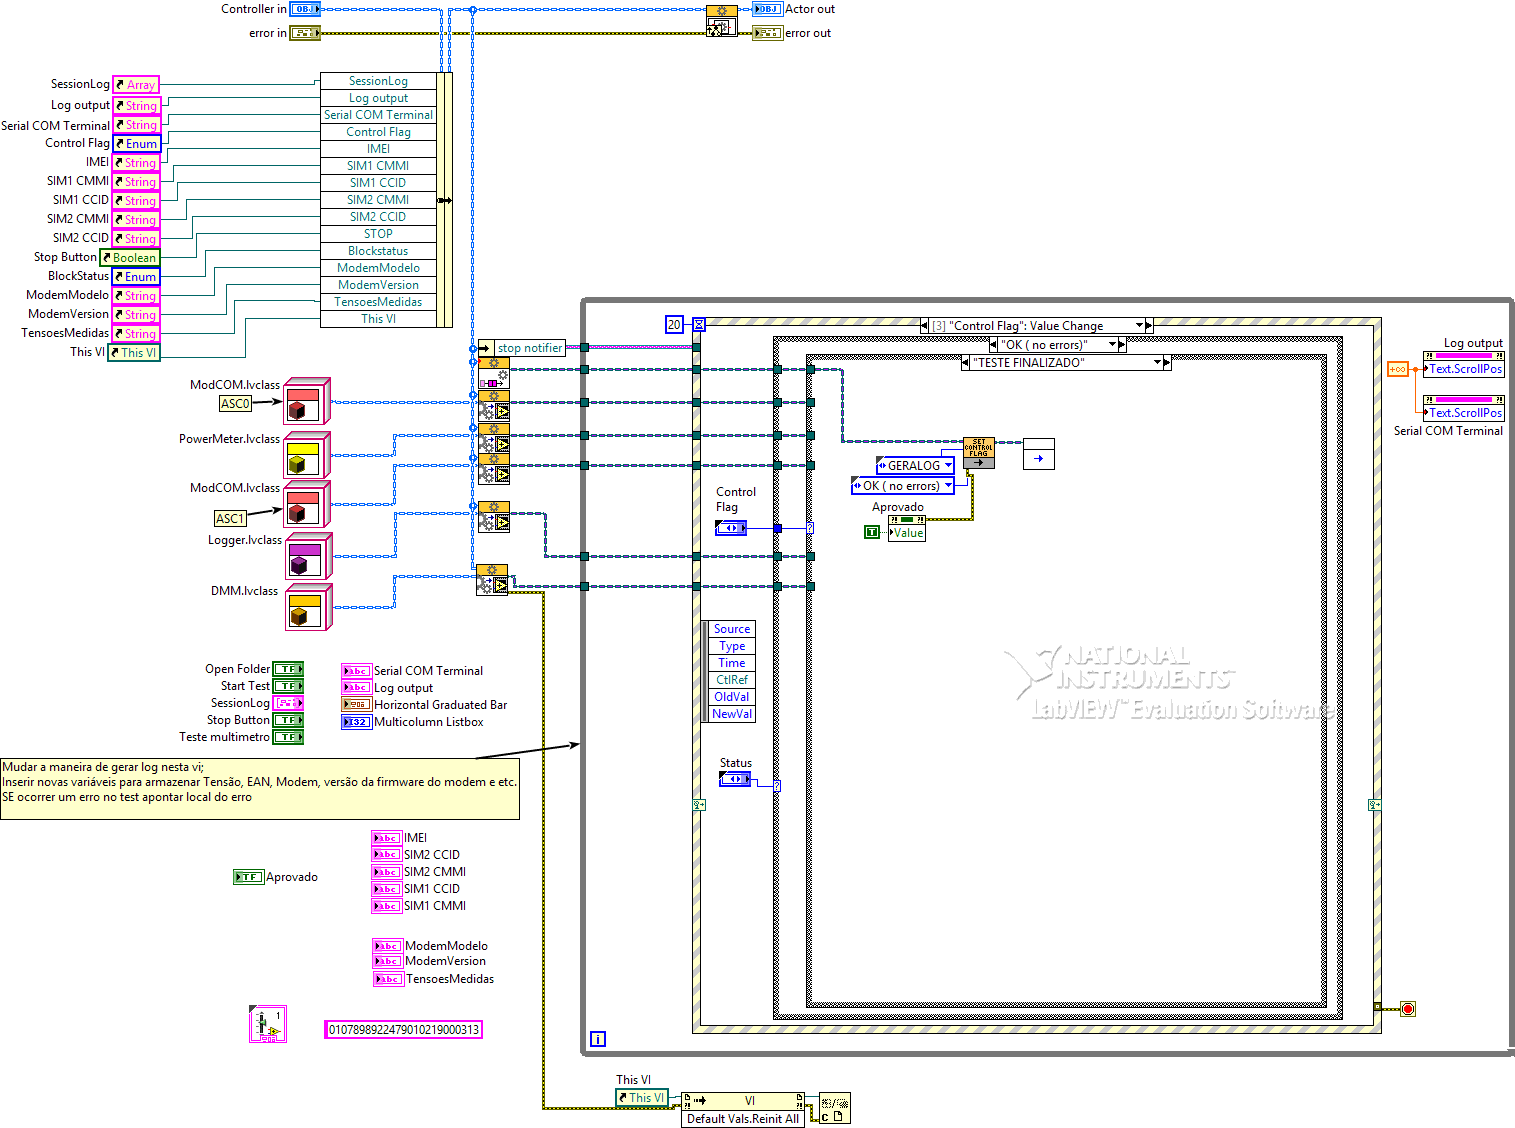
\includegraphics[width=1\linewidth]{lv/controler/Controller_lvclass_Actor_Cored}
                \caption{Diagrama de blocos do \textit{Actor Core.vi} do Controlador}
                \label{fig:cntrlcore}
        \end{figure}
        
        Vemos também na figura \ref{fig:cntrlcore}, que este ator inicializa todos os outros atores filhos logo no inicio de sua execução. Seu inicializador pode ser visto na figura \ref{fig:cntrlprestop}.
        
        Da mesma forma que os atores filhos se comunicam com o controlador pelas mensagens sob sua competência, este só pode enviar mensagens que aqueles possam entender.
        
        \begin{figure}
                \centering
                \begin{subfigure}[b]{0.45\textwidth}
                    \includegraphics[width=1\linewidth]{lv/controler/Controller_lvclass_Pre_Launch_Initd}
                    \caption{VI de pré-inicialização}
                \end{subfigure}
                \begin{subfigure}[b]{0.45\textwidth}
                    \includegraphics[width=\linewidth]{lv/controler/Controller_lvclass_Stop_Cored}
                    \caption{VI de parada}
                \end{subfigure}
                \caption{Capturas de tela das VI de pré-inicialização e parada do Ator}
                \label{fig:cntrlprestop}
        \end{figure}
        
        \begin{figure}
                \centering
                \includegraphics[width=0.9\linewidth]{lv/controler/Controller_lvclass_SET_Control_Flagd}
                \caption{Captura de tela do método interno que recebe a mensagem do bloco de teste executado e seu status de conclusão.}
                \label{fig:cntrlset}
        \end{figure}
        
    
        \clearpage
    \clearpage
    \chapter{Análise de execução}
    
        Com o programa pronto, foi montado um esquema de teste internamente, sem que fosse à fábrica, para avaliá-lo em relação à versão anterior em Java. Foram separadas cerca de 20 placas e testadas com ambos os programas.
        
        Após isso, foram mensurados os tempos de execução de teste. A figura \ref{tab:resultado} exibe as médias dos resultados para os dois programas. Nota-se pela imagem, uma redução de quase 10 segundos no tempo médio de teste. Observa-se que estes resultados são atribuídos somente pelas mudanças ergonômicas do programa, já que o roteiro é idêntico ao anterior. Questões de velocidade de processamento entre as linguagens não refletiram em muitas mudanças, se considerarmos que nenhuma das atividades exigem uso intenso de CPU, e que o gargalo do teste é interno ao modem. Certamente que resultados melhores podem ser obtidos se aproveitados os recursos de concorrência de \textit{software} que \textit{framework} oferece. Isso foge do escopo deste trabalho, que se propôs somente em oferecer uma base para o teste concorrente de placas eletrônicas.
        
    \begin{table}[]
        \centering
        \caption{Média e desvio padrão das 20 amostras de teste de bancada}
        \label{tab:resultado}
        \begin{tabular}{l|cc}
        
                          & Programa Legado & Modelo de Atores \\
    \hline
            Média (seg)         & $33.65\pm2.43$          & $26.24\pm3.37$                          \\
        \end{tabular}
        \end{table}
        
    \begin{comment}
        Com o programa pronto, foi montado um esquema de teste para avaliá-lo em relação à versão anterior em Java. 
        Foi separado um lote de 200 placas e testadas metade com o primeiro programa, e outra metade com o outro.
        
        A partir destes estados, foram levantados os tempos de execução de cada teste que são exibidos na figura \ref{fig:resultado}. Observa-se pela imagem, uma redução considerável no tempo mínimo e médio de teste. Passando de 
        
        Observa-se que estes resultados foram obtidos somente com a mudança de uma linguagem interpretada para uma compilada, e melhor elaboração do programa, Já que o roteiro é idêntico ao anterior. Certamente que resultados melhores podem ser obtidos se aproveitados os recursos de concorrência de \textit{software} que \textit{framework} oferece. 
        
        Nota-se também que a distribuição dos tempos de teste do programa novo é ligeiramente mais difusas do que o do programa antigo, que pode ser atribuído à falta de hábito dos operários com a nova interface.
        
        Também foram observados a quantidade de erros existentes no programa durante as etapas que envolvem interação com o operador. Esses erros analisados estão aqui representados na figura \ref{fig:erros}. Como esperado, melhorias ergonômicas reduziram o tempo de teste, e taxa de erro de operador.
        
        
        \begin{figure}
            \centering
            \includegraphics{}
            \caption{taxa de erro nas baterias de teste que envolvem o operador}
            \label{fig:erros}
        \end{figure}
\end{comment}        

   \section{Conclusão}
       
        
        Neste trabalho, não foi realizada nenhuma análise crítica do roteiro de testes e sua efetividade de cobertura. Isso se torna imprescindível, considerando os dados internos da manutenção que frequentemente reportam \textit{"causa desconhecida"} sobre os retornos de campo.
        
        O uso da linguagem gráfica do ambiente \textit{Labview} apesar de simples para pequenas rotinas, torna-se complicado e difícil de refatorar ao aplicado a programas maiores, e sua implementação do paradigma orientado à objetos assim como do modelo de atores é demasiadamente complicada e problemática de usar.
        Uma maneira de contornar isto seria, talvez a utilização do Labwindows\texttrademark/CVI, o ambiente C da National Instruments, ou o uso do Labview somente em partes aonde ele se sobressalta como melhor opção.
        
        O principal problema encontrado foi o escrever o roteiro da bateria de testes no código fonte do programa. Isso inflexibiliza a equipe em relação à mudanças
        
        Dentre as melhorias interessantes para o processos de teste de placas, destacam-se:
        \begin{itemize}
            \item Paralelização do roteiro e melhor uso dos recursos da concorrência de software.
            \item Roteiro como arquivo de entrada do programa, interpretado por um módulo interno do programa.
            \item Envio automático e criptografado do roteiro ao sistema de registros de teste da fábrica. Atualmente isso é realizado manualmente.
            \item Teste de potência RF serem realizados em conjunto com os testes em fábrica.
            \item Construção de uma giga de testes que suporte múltiplas placas sendo testadas simultaneamente. No aspecto de software, isso demandaria o desenvolvimento de um ator numa camada superior ao controlador - tarefa sem grandes dificuldades.
        \end{itemize}
        
        Feitas as críticas, ressalta-se que o modelo de atores se mostrou apropriado para modelar vários módulos de software concorrentes, e escalona bem para aplicações maiores. 
        
    
% ----------------------------------------------------------
% ELEMENTOS PÓS-TEXTUAIS
% ----------------------------------------------------------
\postextual
% ----------------------------------------------------------

%\bibliographystyle{plain}
\bibliographystyle{apalike}

\bibliography{references}
\end{document}

% --- 
% https://github.com/mateusduboli/ufsc-thesis-latex
% ---------------------------------------------------------
